% !TEX root = ../thesis.tex

\section{Fit Validation and Bias Testing}
\label{sec:bias}

% Fit validation overview
The nuisance parameters implemented as part of the 2D fitting process for each of the 24 categories results in various alternative shapes for the signal and background models.
To check their performance, we perform various fit validation and bias tests to evaluate the quality of the 2D fit, which includes the correctness of the shape uncertainties. % Check wording
We consider the post-fit pulls and impacts for each of the nuisance parameters described in section~\ref{sec:uncert}, post-fit distributions for a background-only fit in the signal region, a goodness-of-fit test using the saturated model algorithm, and a signal-injected bias test using a maximum likelihood fit.

\subsection{Post-fit Pulls and Impacts}

% Post-fit pulls
One of the tests performed examines the behavior of the nuisance parameters in a background-only fit and a signal+background fit for a given signal model and specified mass, with the signal cross section free to float, but without looking at its measured value prior to unblinding.
We then compare the final post-fit values and uncertainties of the nuisance parameters to the pre-fit values and uncertainties, which can be seen in figure~\ref{fig:nuisances}.
Most post-fit nuisance parameters fall within the $\pm1\sigma$ range of their pre-fit values, with some larger deviations in parameters related to the jet \pt spectrum.

% Pulls and impacts
We also consider the post-fit pull and impact of each parameter on the measured signal cross section for both a non-\VBF and \VBF signal in figures~\ref{fig:impacts_WprToWH} and \ref{fig:impacts_VBFRadToWW}.
The pulls are defined as the difference between the pre- and pos-fit values divided by the pre-fit uncertainty for a given nuisance parameter, and the impacts are defined as the shift $\Delta r$ of the measured signal cross section obtained by fixing the nuisance parameter to its $+1\sigma$ or $-1\sigma$ post-fit values while all other parameters are profiled.
Figures~\ref{fig:impacts_WprToWH} and \ref{fig:impacts_VBFRadToWW} show the resulting post-fit pulls and impacts for a non-\VBF and \VBF signal, respectively.
The resulting impacts are relatively small and range from $10^{-3}$ to $10^{-6}$.

\begin{figure}[htbp]
  \centering
  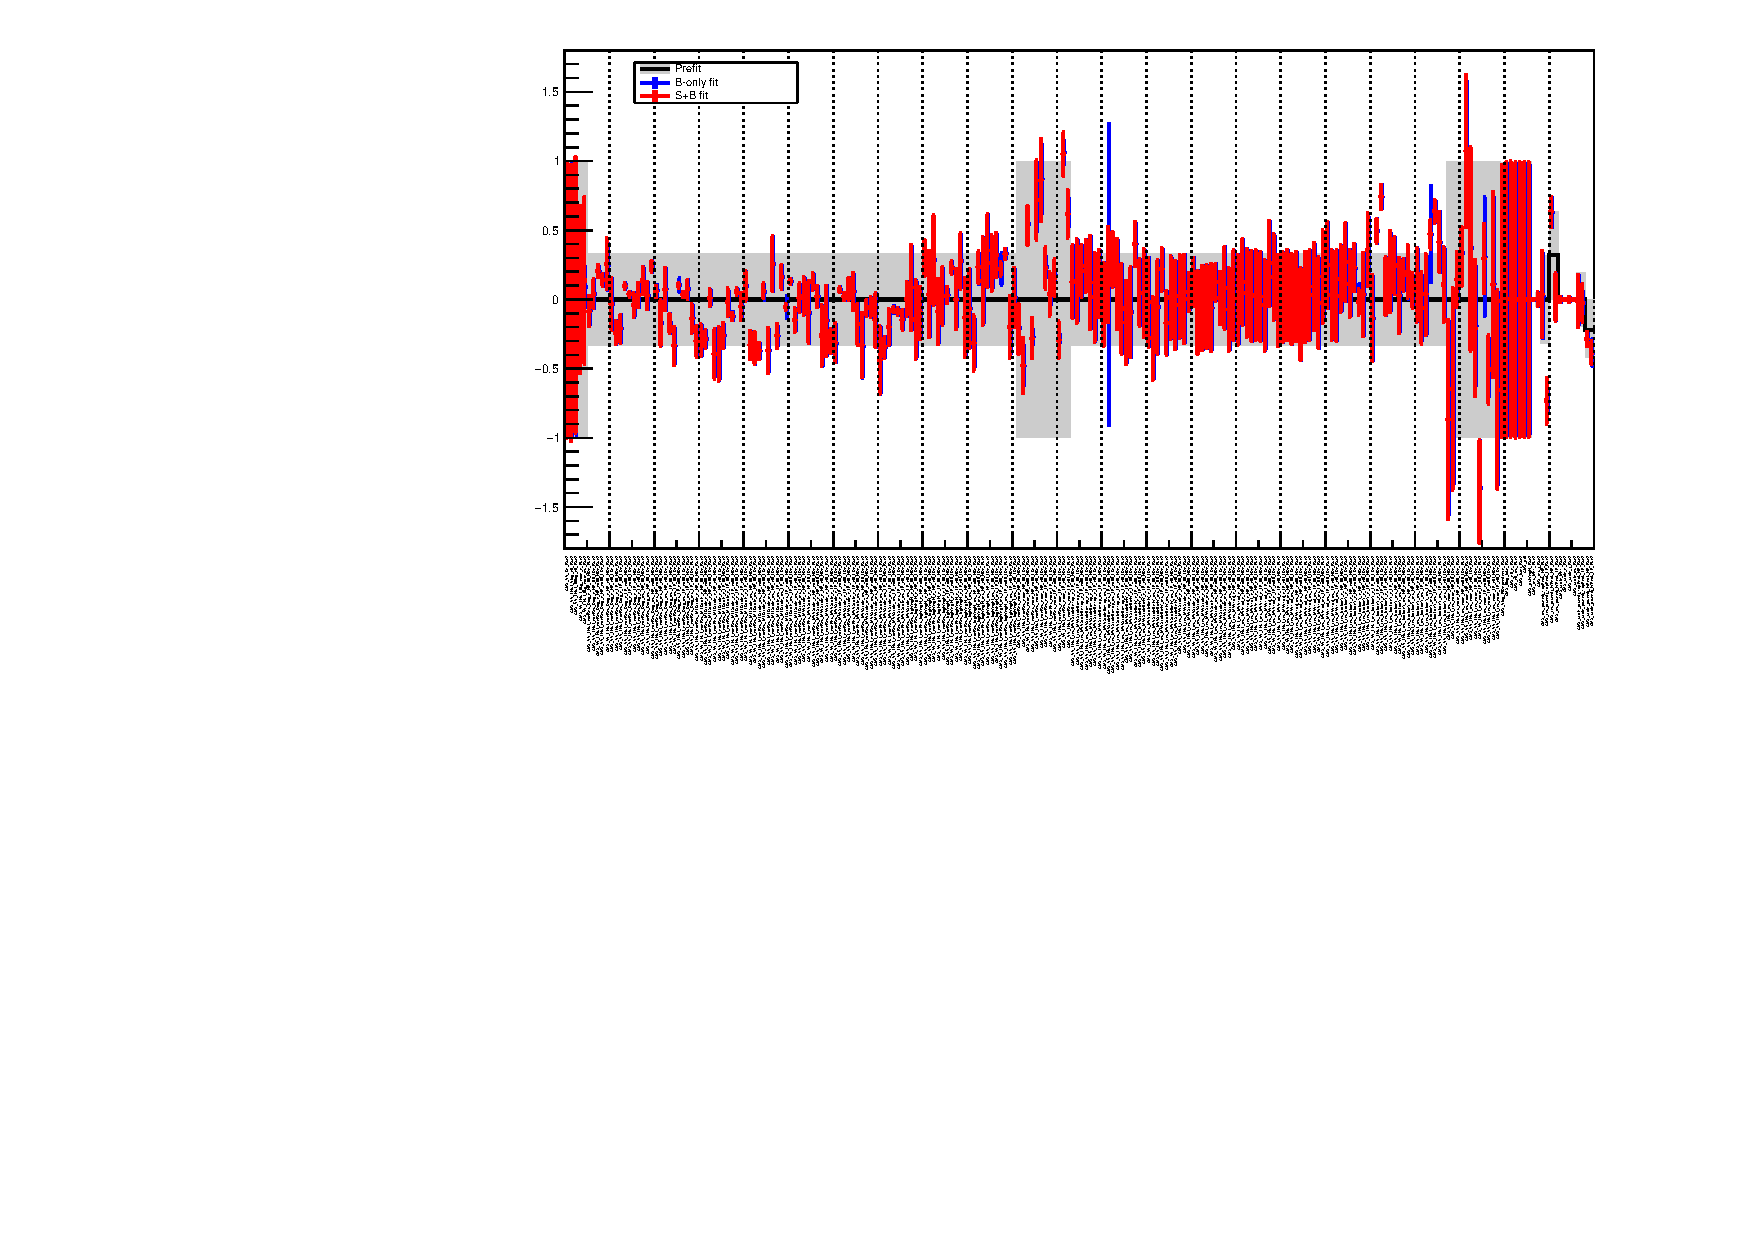
\includegraphics[width=0.95\textwidth,angle=270]{fig/fitValidation/nuisances_WprToWH1000.pdf}
  \caption{
    Comparison of the post-fit values and uncertainties for each nuisance parameter with respect to their pre-fit values and uncertainties for background-only and signal+background fits using the \DY\WprtoWH model with $m_{\Wpr}=1\unit{TeV}$.
    Gray bands and blue/red bars represent $\pm\sigma$ pre- and post-fit uncertainties, respectively.
  }
  \label{fig:nuisances}
\end{figure}

\begin{figure}[htbp]
  \centering
  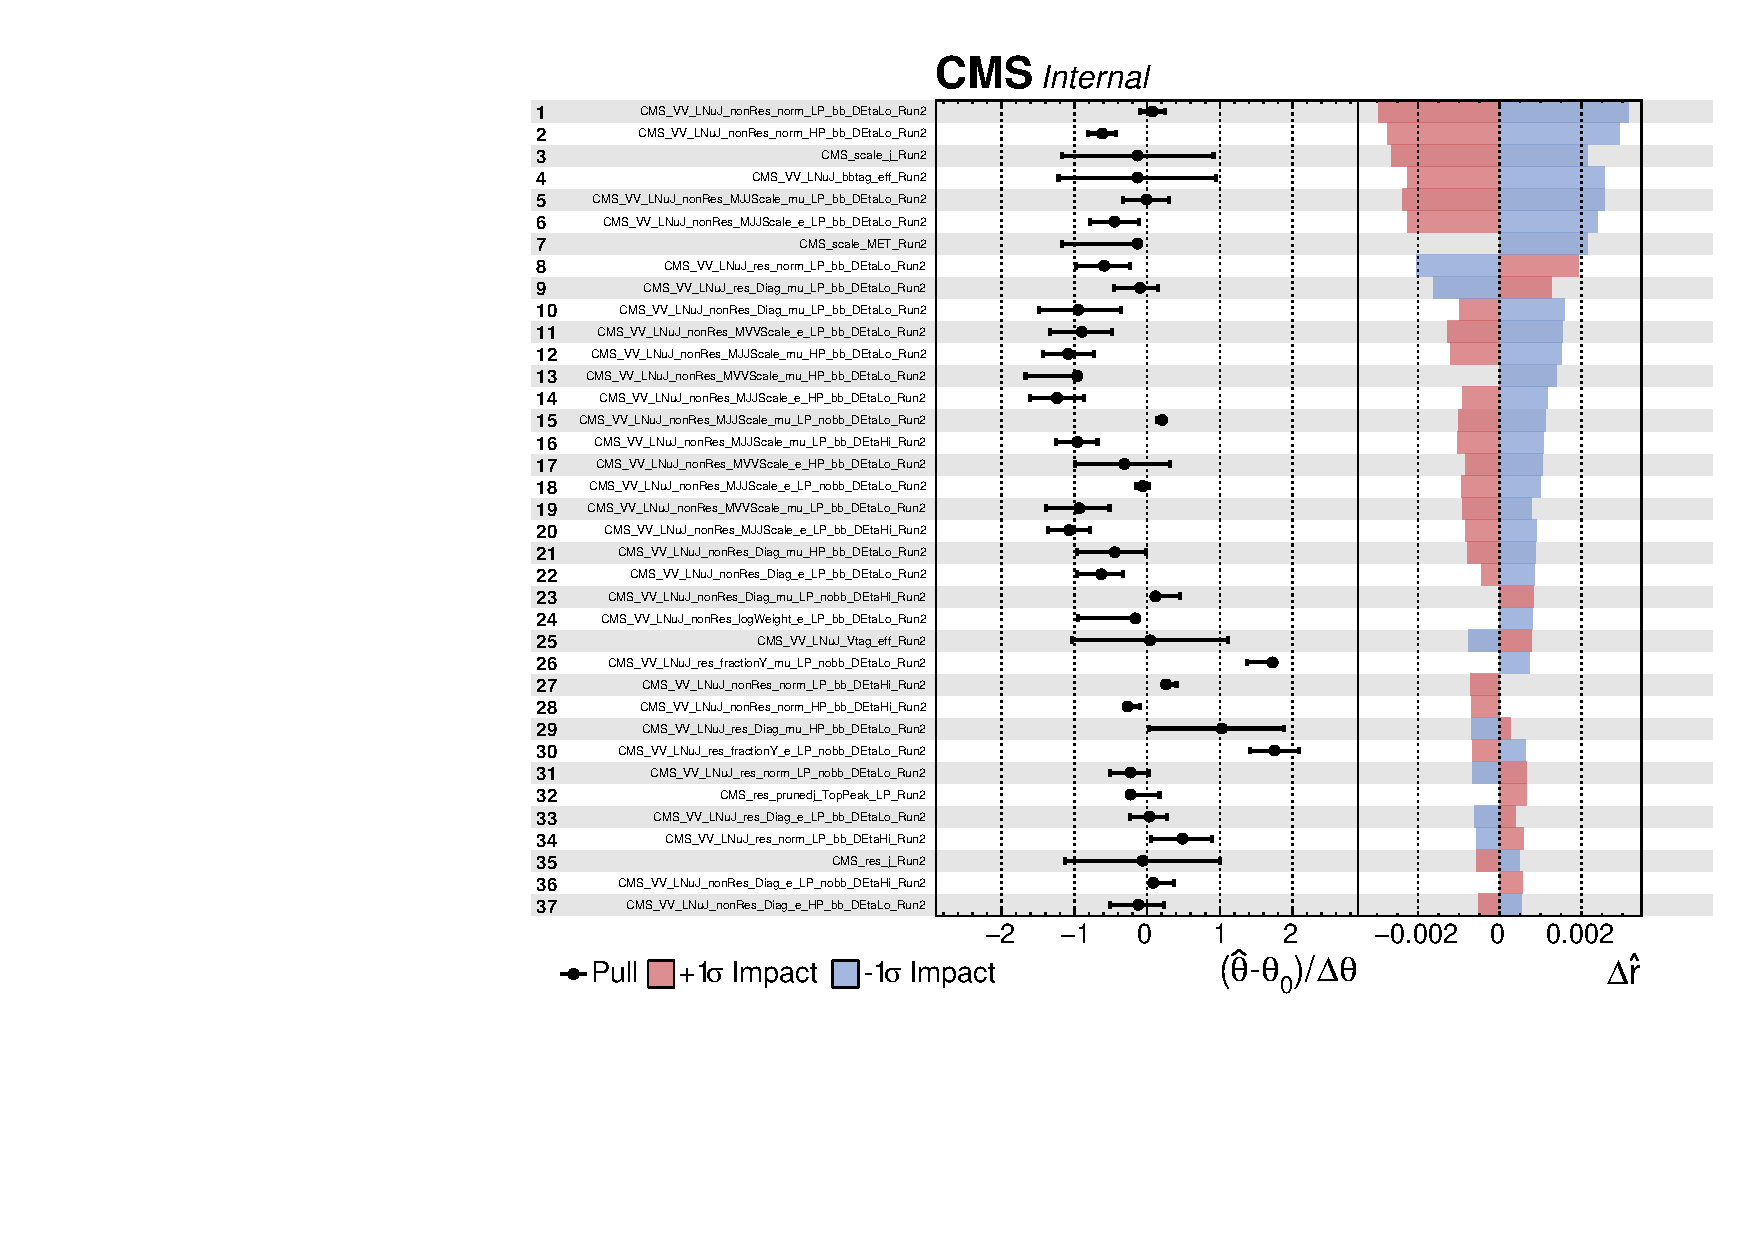
\includegraphics[width=0.45\textwidth,page=1]{fig/fitValidation/impacts_WprToWH1000_6p_72.pdf}
  \includegraphics[width=0.45\textwidth,page=2]{fig/fitValidation/impacts_WprToWH1000_6p_72.pdf}\\
  \includegraphics[width=0.45\textwidth,page=3]{fig/fitValidation/impacts_WprToWH1000_6p_72.pdf}
  \includegraphics[width=0.45\textwidth,page=4]{fig/fitValidation/impacts_WprToWH1000_6p_72.pdf}\\
  \includegraphics[width=0.45\textwidth,page=5]{fig/fitValidation/impacts_WprToWH1000_6p_72.pdf}
  \includegraphics[width=0.45\textwidth,page=6]{fig/fitValidation/impacts_WprToWH1000_6p_72.pdf}\\
  \caption{
    Pulls of the nuisance parameters, and impacts of a shift for each nuisance parameter on the measured signal cross section for the \DY\WprtoWH model with $m_{\Wpr}=1\unit{TeV}$.
  }
  \label{fig:impacts_WprToWH}
\end{figure}

\begin{figure}[htbp]
  \centering
  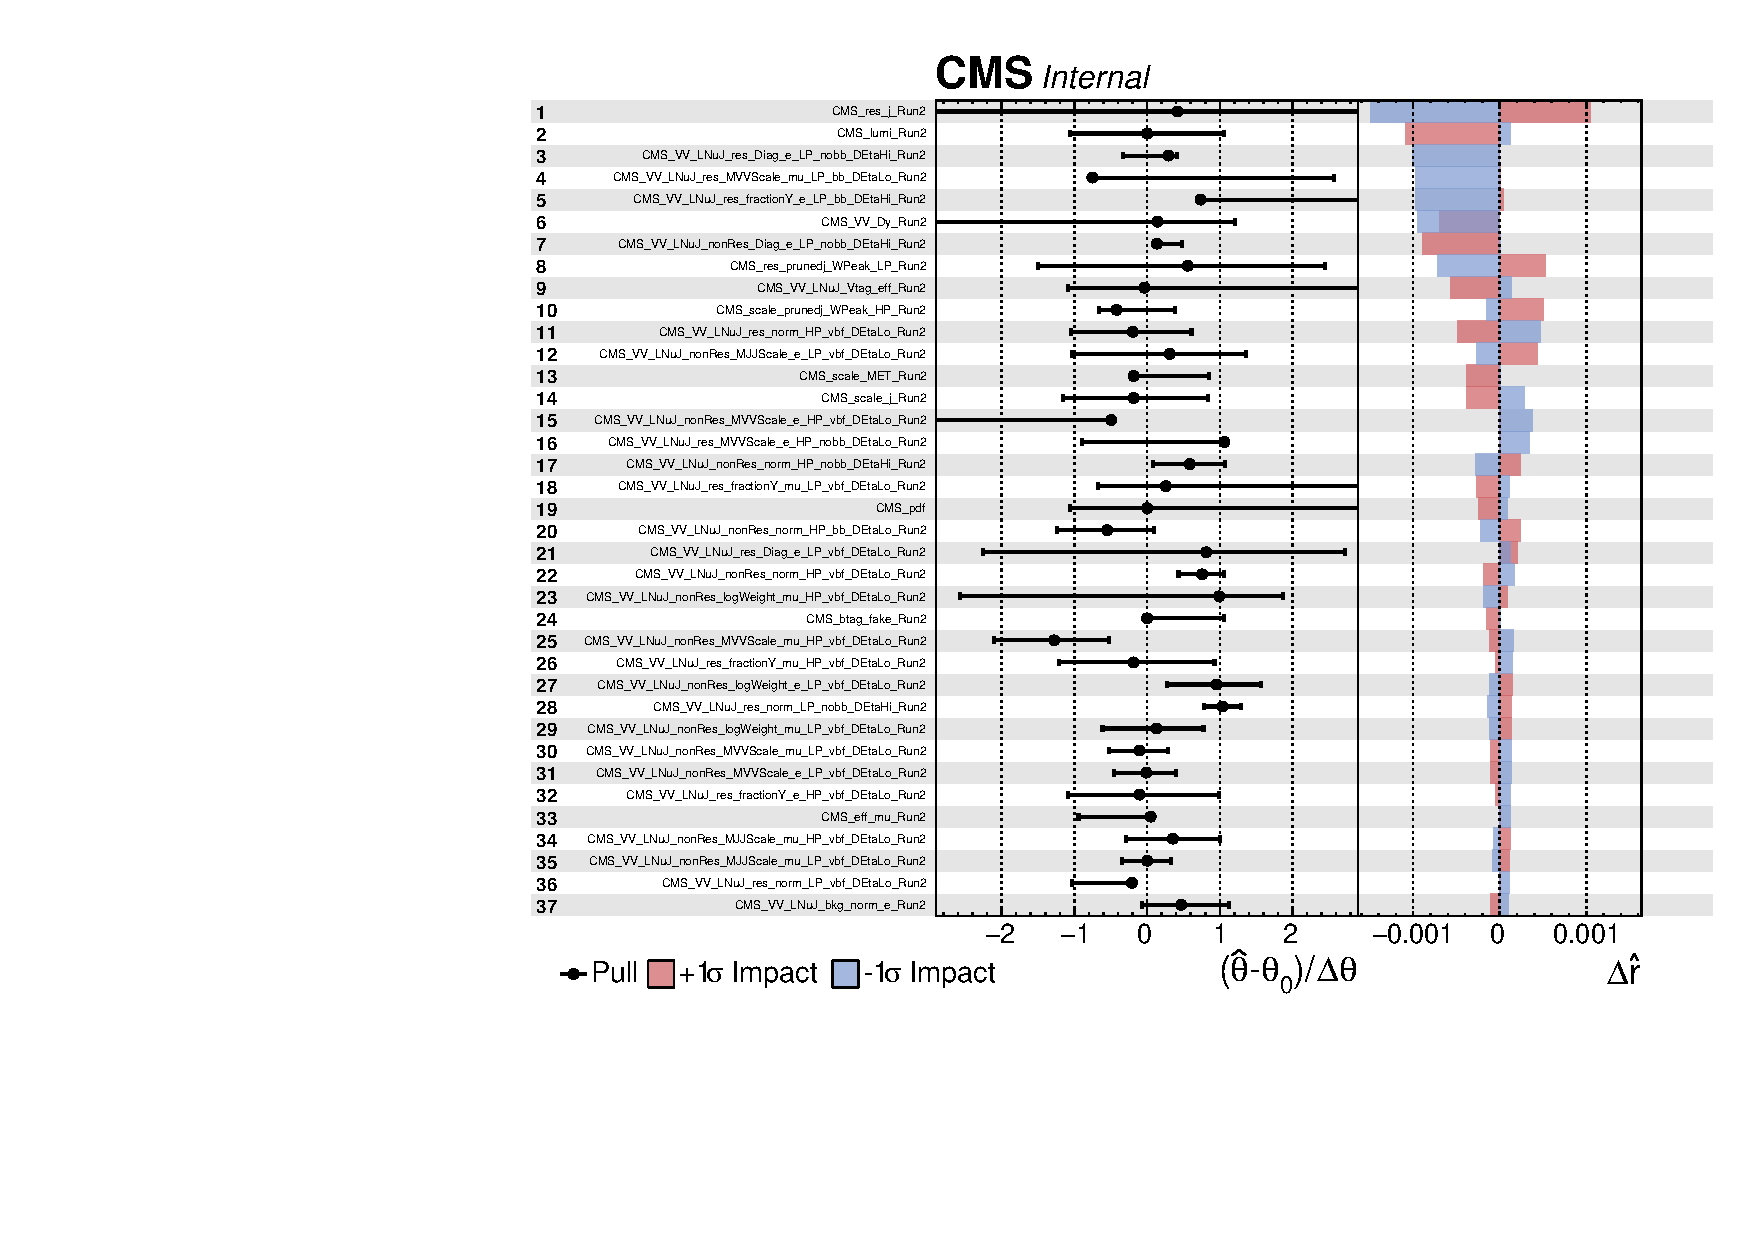
\includegraphics[width=0.45\textwidth,page=1]{fig/fitValidation/impacts_VBFRadToWW1000_6p_72.pdf}
  \includegraphics[width=0.45\textwidth,page=2]{fig/fitValidation/impacts_VBFRadToWW1000_6p_72.pdf}\\
  \includegraphics[width=0.45\textwidth,page=3]{fig/fitValidation/impacts_VBFRadToWW1000_6p_72.pdf}
  \includegraphics[width=0.45\textwidth,page=4]{fig/fitValidation/impacts_VBFRadToWW1000_6p_72.pdf}\\
  \includegraphics[width=0.45\textwidth,page=5]{fig/fitValidation/impacts_VBFRadToWW1000_6p_72.pdf}
  \includegraphics[width=0.45\textwidth,page=6]{fig/fitValidation/impacts_VBFRadToWW1000_6p_72.pdf}\\
  \caption{
    Pulls of the nuisance parameters, and impacts of a shift for each nuisance parameter on the measured signal cross section for the \VBF\RadtoWW model with $m_{\Rad}=1\unit{TeV}$.
  }
  \label{fig:impacts_VBFRadToWW}
\end{figure}

\subsection{Post-fit Distributions}

% Post-fit distributions
Another test performed to assess the fit quality involves performing a background-only fit and plotting post-fit distributions in the signal region.
Figure~\ref{fig:postfit_MJJ_Run2} shows the post-fit distributions for all categories projected onto the \MJ dimension for all events in the full range of \MVV, while figure~\ref{fig:postfit_MVV_Run2} shows the post-fit distributions projected onto the \MVV dimension for all events in the full \MJ range.
We also consider slices of \MJ and \MVV while projecting over the full range of the other variable.
Figures~\ref{fig:postfit_MJJ_MVV0700to1000_Run2}, \ref{fig:postfit_MJJ_MVV1000to1500_Run2}, and \ref{fig:postfit_MJJ_MVV1500to5000_Run2} show the post-fit distributions for the low ($[0.7,1.0\unit{TeV}]$), medium ($[1.0,1.5\unit{TeV}]$), and high ($[1.5,5.0\unit{TeV}]$) \MVV ranges projected into the \MJ dimension, respectively.
We do the same in figures~\ref{fig:postfit_MVV_MJJ020to070_Run2}, \ref{fig:postfit_MVV_MJJ070to110_Run2}, \ref{fig:postfit_MVV_MJJ110to150_Run2}, and \ref{fig:postfit_MVV_MJJ150to210_Run2} for the low jet mass sideband ($\MJ<70\unit{GeV}$), $W/Z$ peak range ($70\leq\MJ\leq110\unit{GeV}$), Higgs boson peak range ($110\leq\MJ\leq150\unit{GeV}$), and high jet mass sideband ($\MJ>150\unit{GeV}$).
Good agreement between the data and post-fit templates is observed for all 24 categories.

\begin{figure}[htbp]
  \centering
  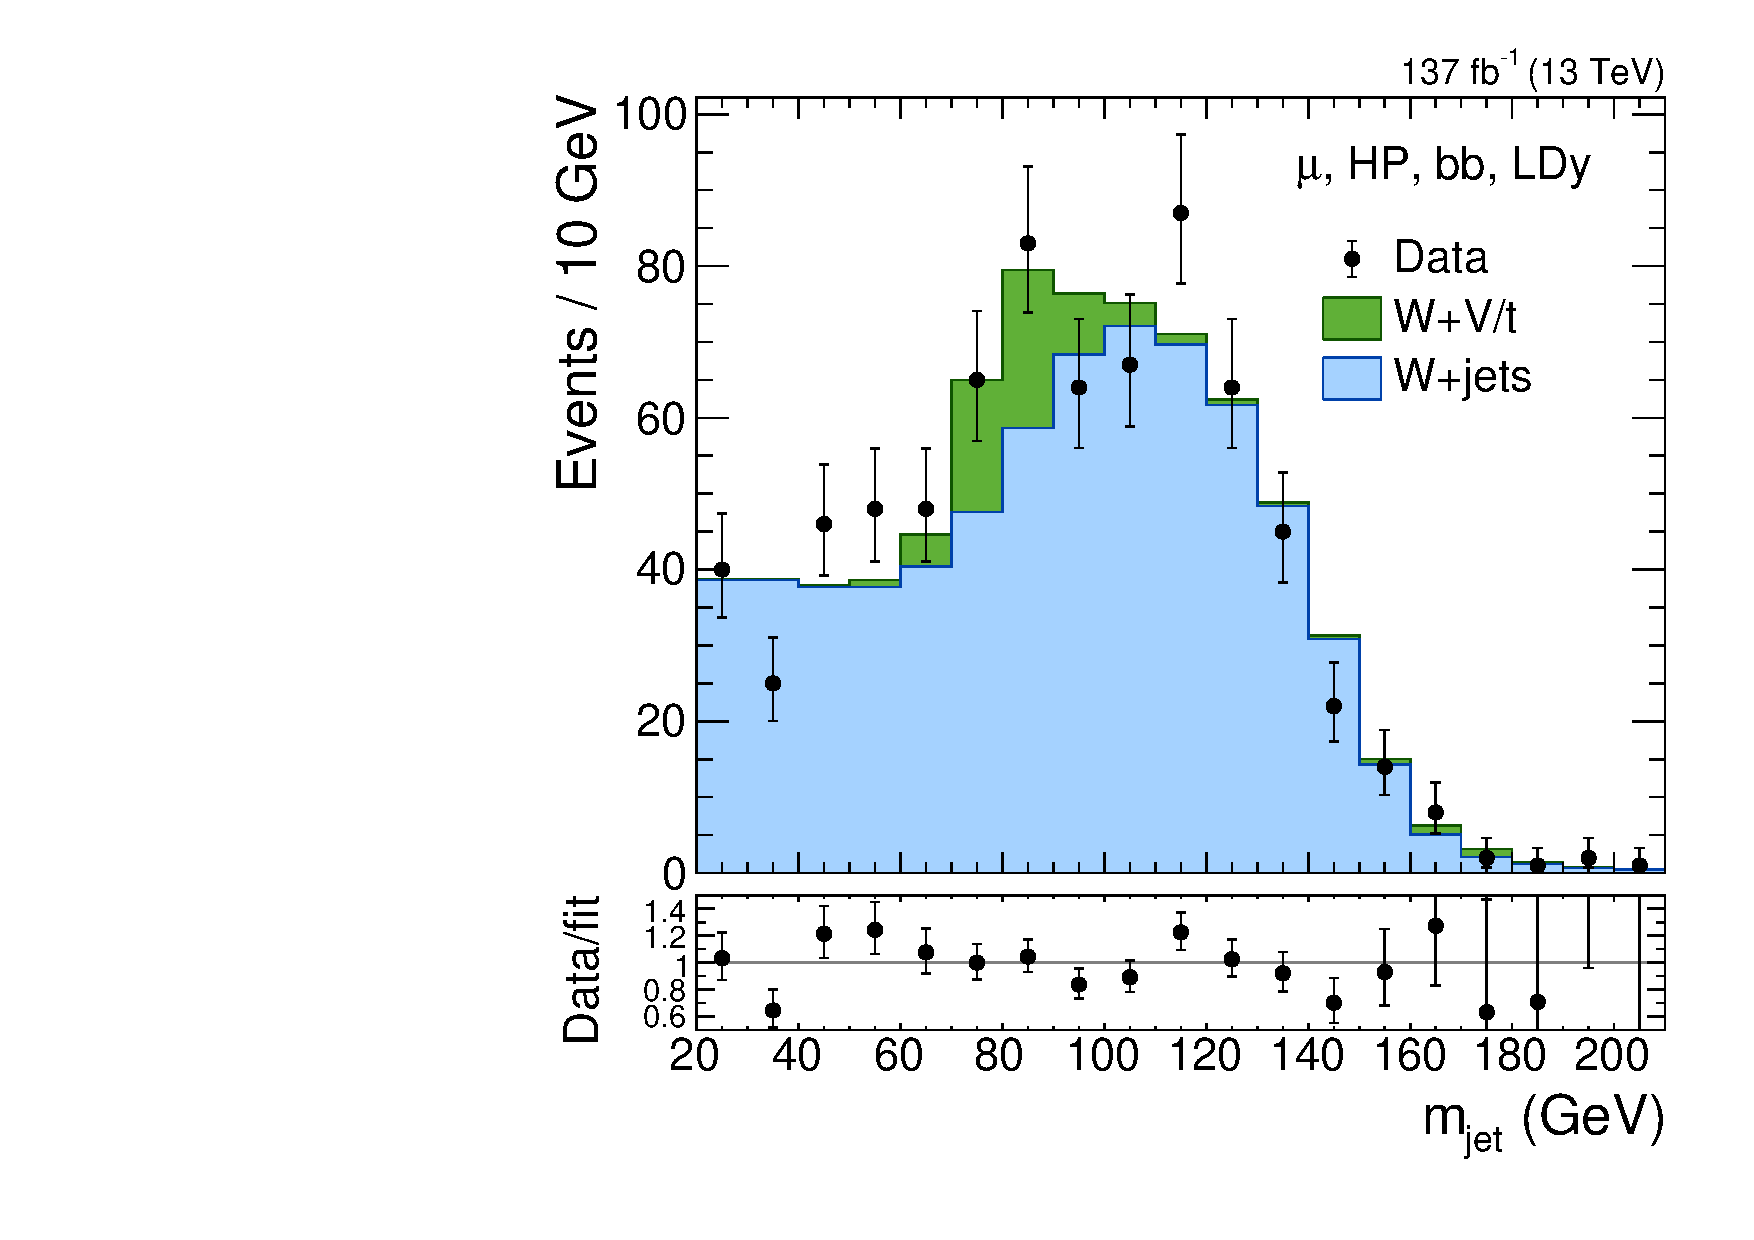
\includegraphics[width=0.18\textwidth]{fig/fitValidation/PostFit_SR_MJJ__mu_HP_bb_LDy_Run2.pdf}
  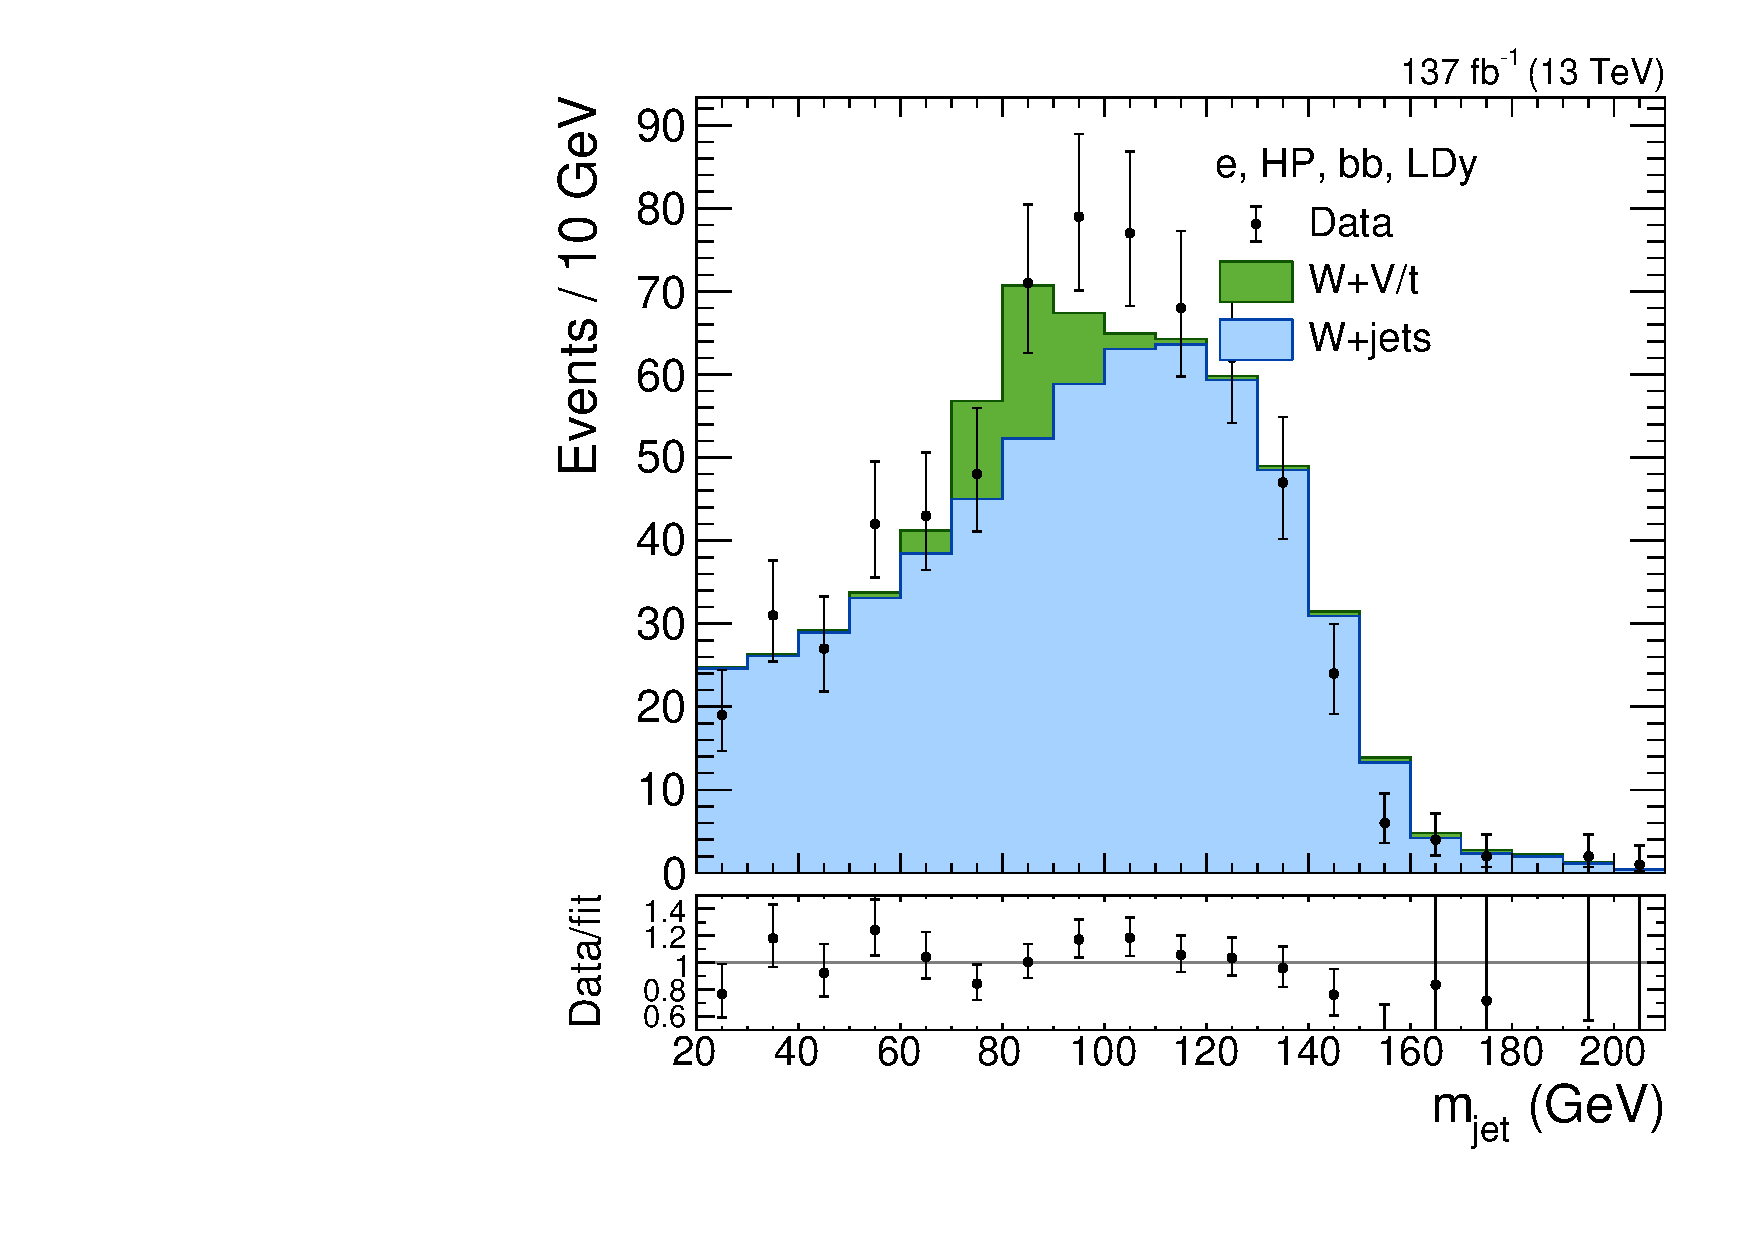
\includegraphics[width=0.18\textwidth]{fig/fitValidation/PostFit_SR_MJJ__e_HP_bb_LDy_Run2.pdf}
  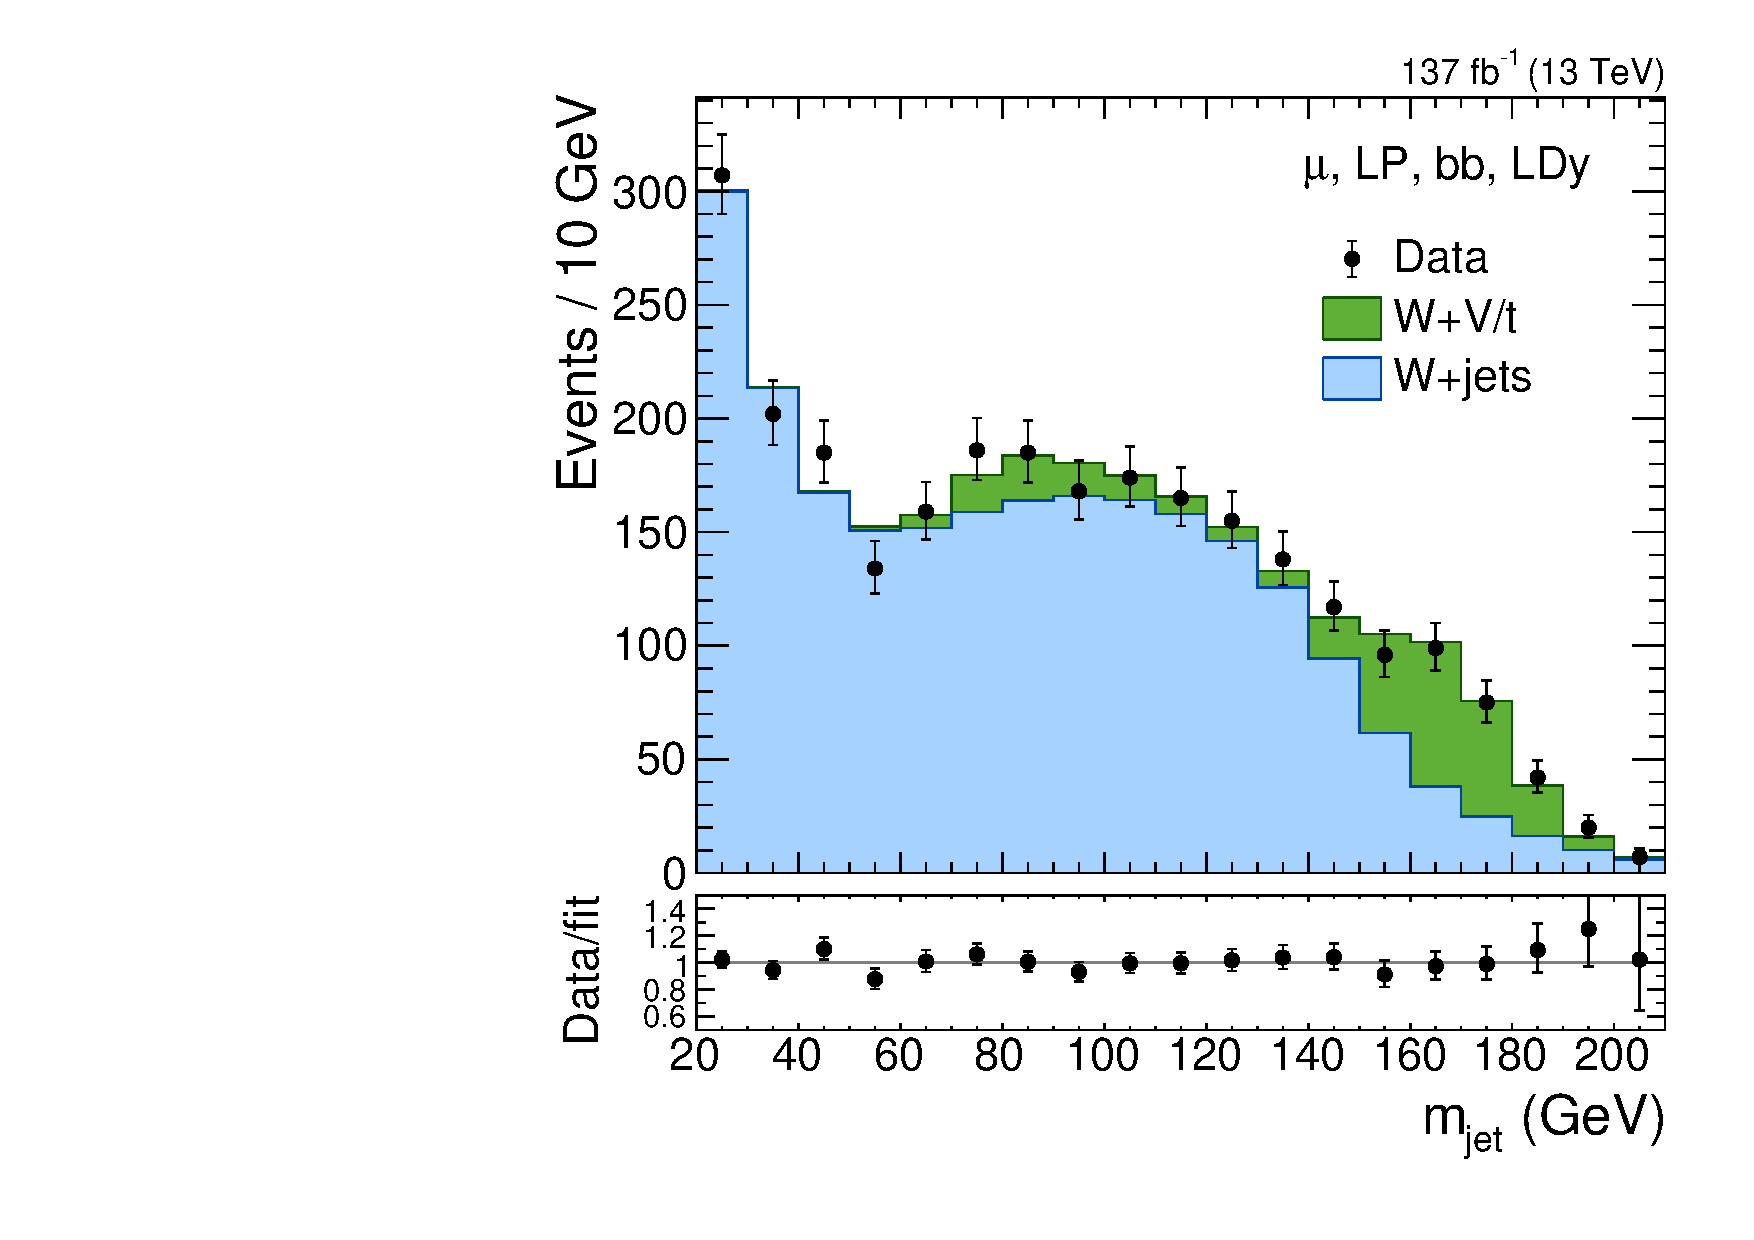
\includegraphics[width=0.18\textwidth]{fig/fitValidation/PostFit_SR_MJJ__mu_LP_bb_LDy_Run2.pdf}
  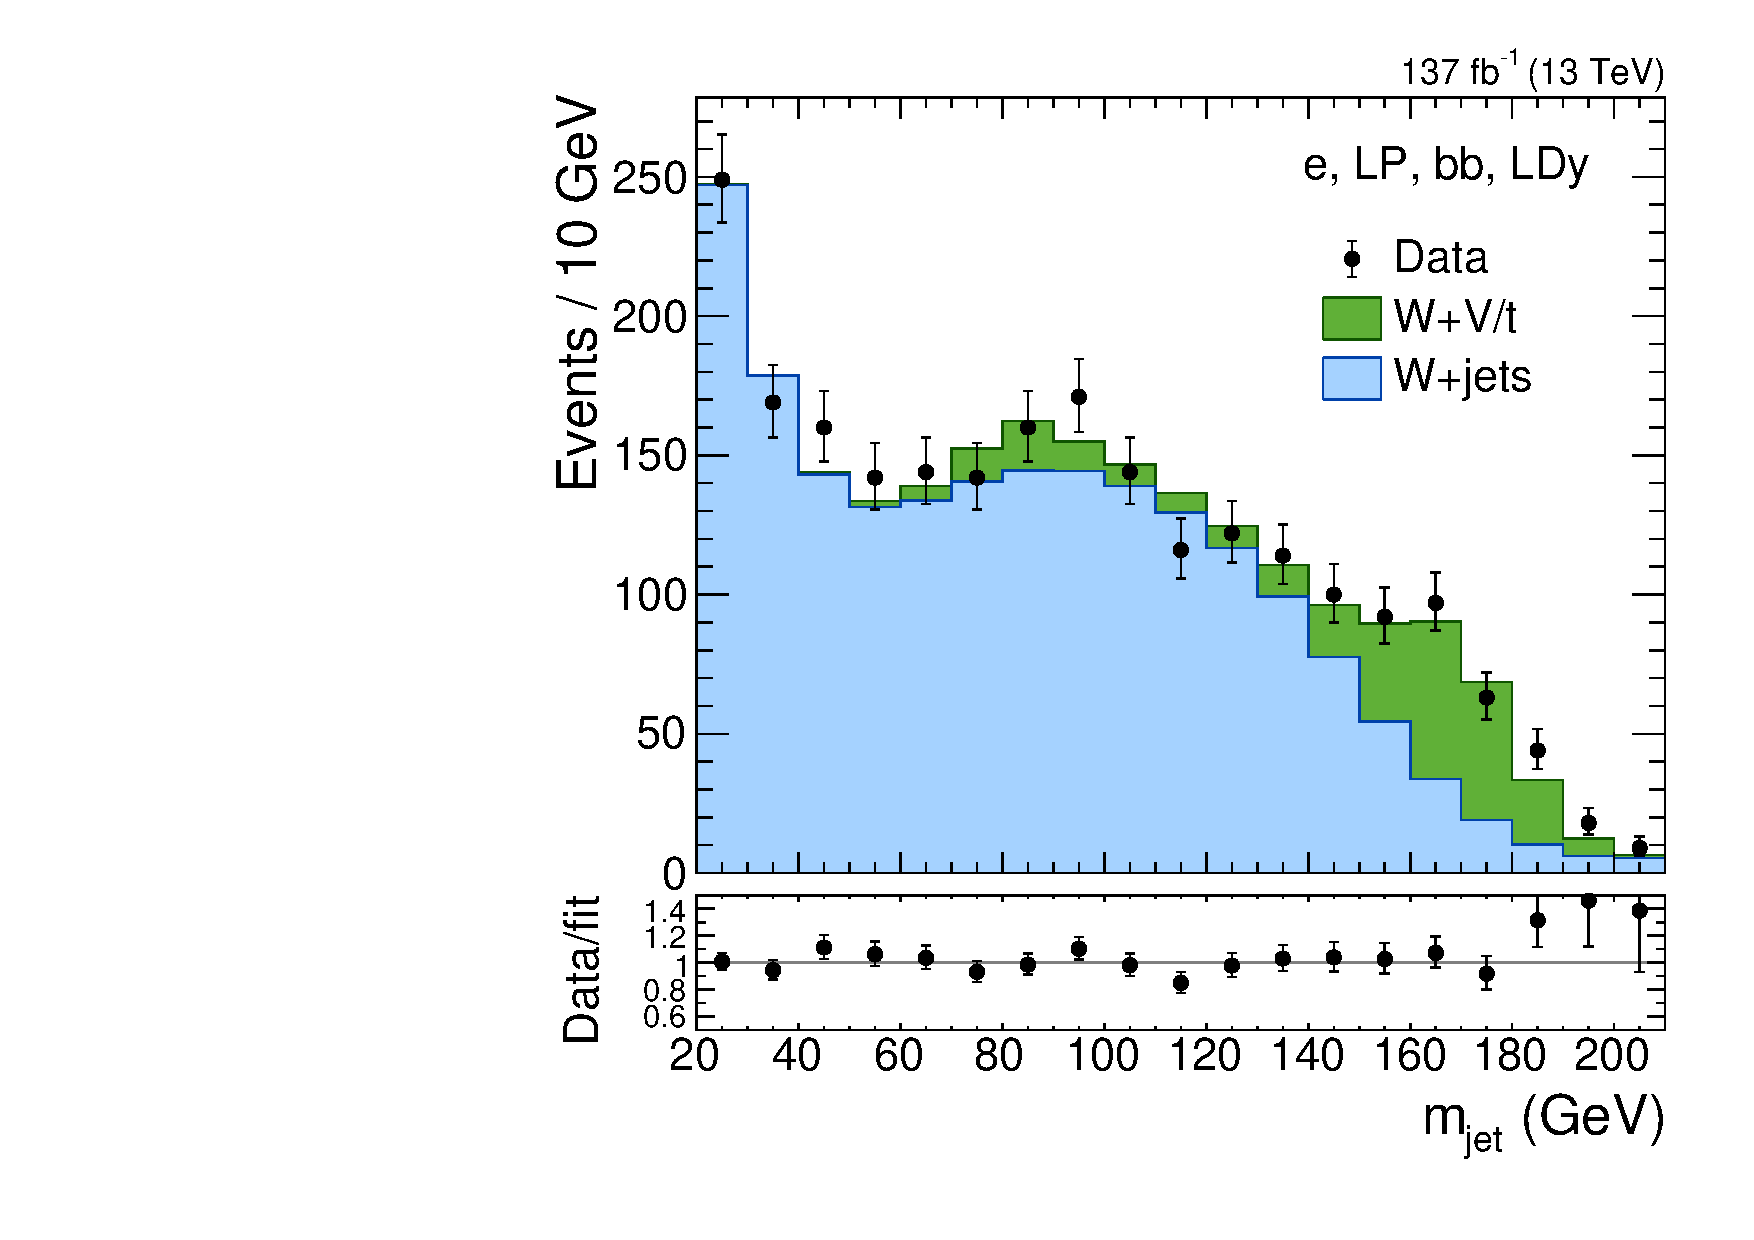
\includegraphics[width=0.18\textwidth]{fig/fitValidation/PostFit_SR_MJJ__e_LP_bb_LDy_Run2.pdf}\\
  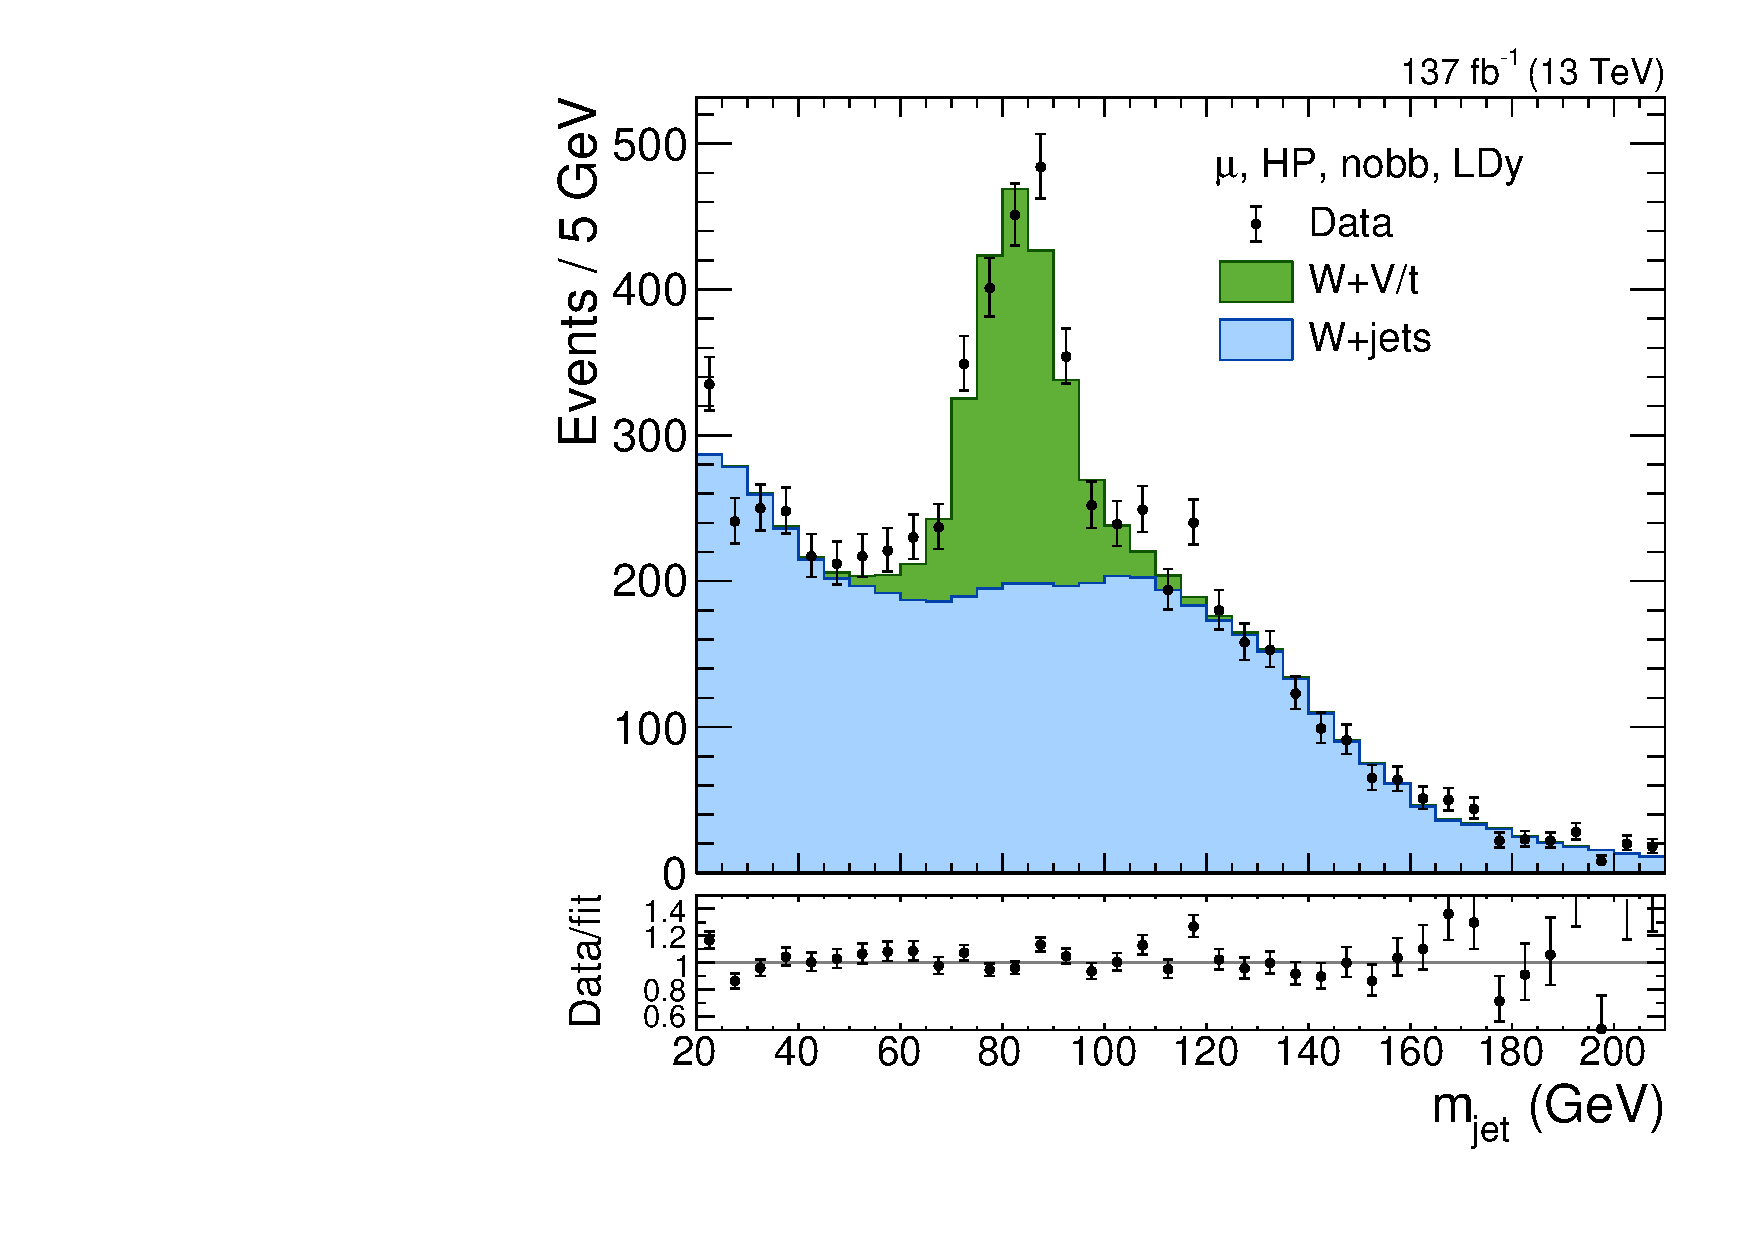
\includegraphics[width=0.18\textwidth]{fig/fitValidation/PostFit_SR_MJJ__mu_HP_nobb_LDy_Run2.pdf}
  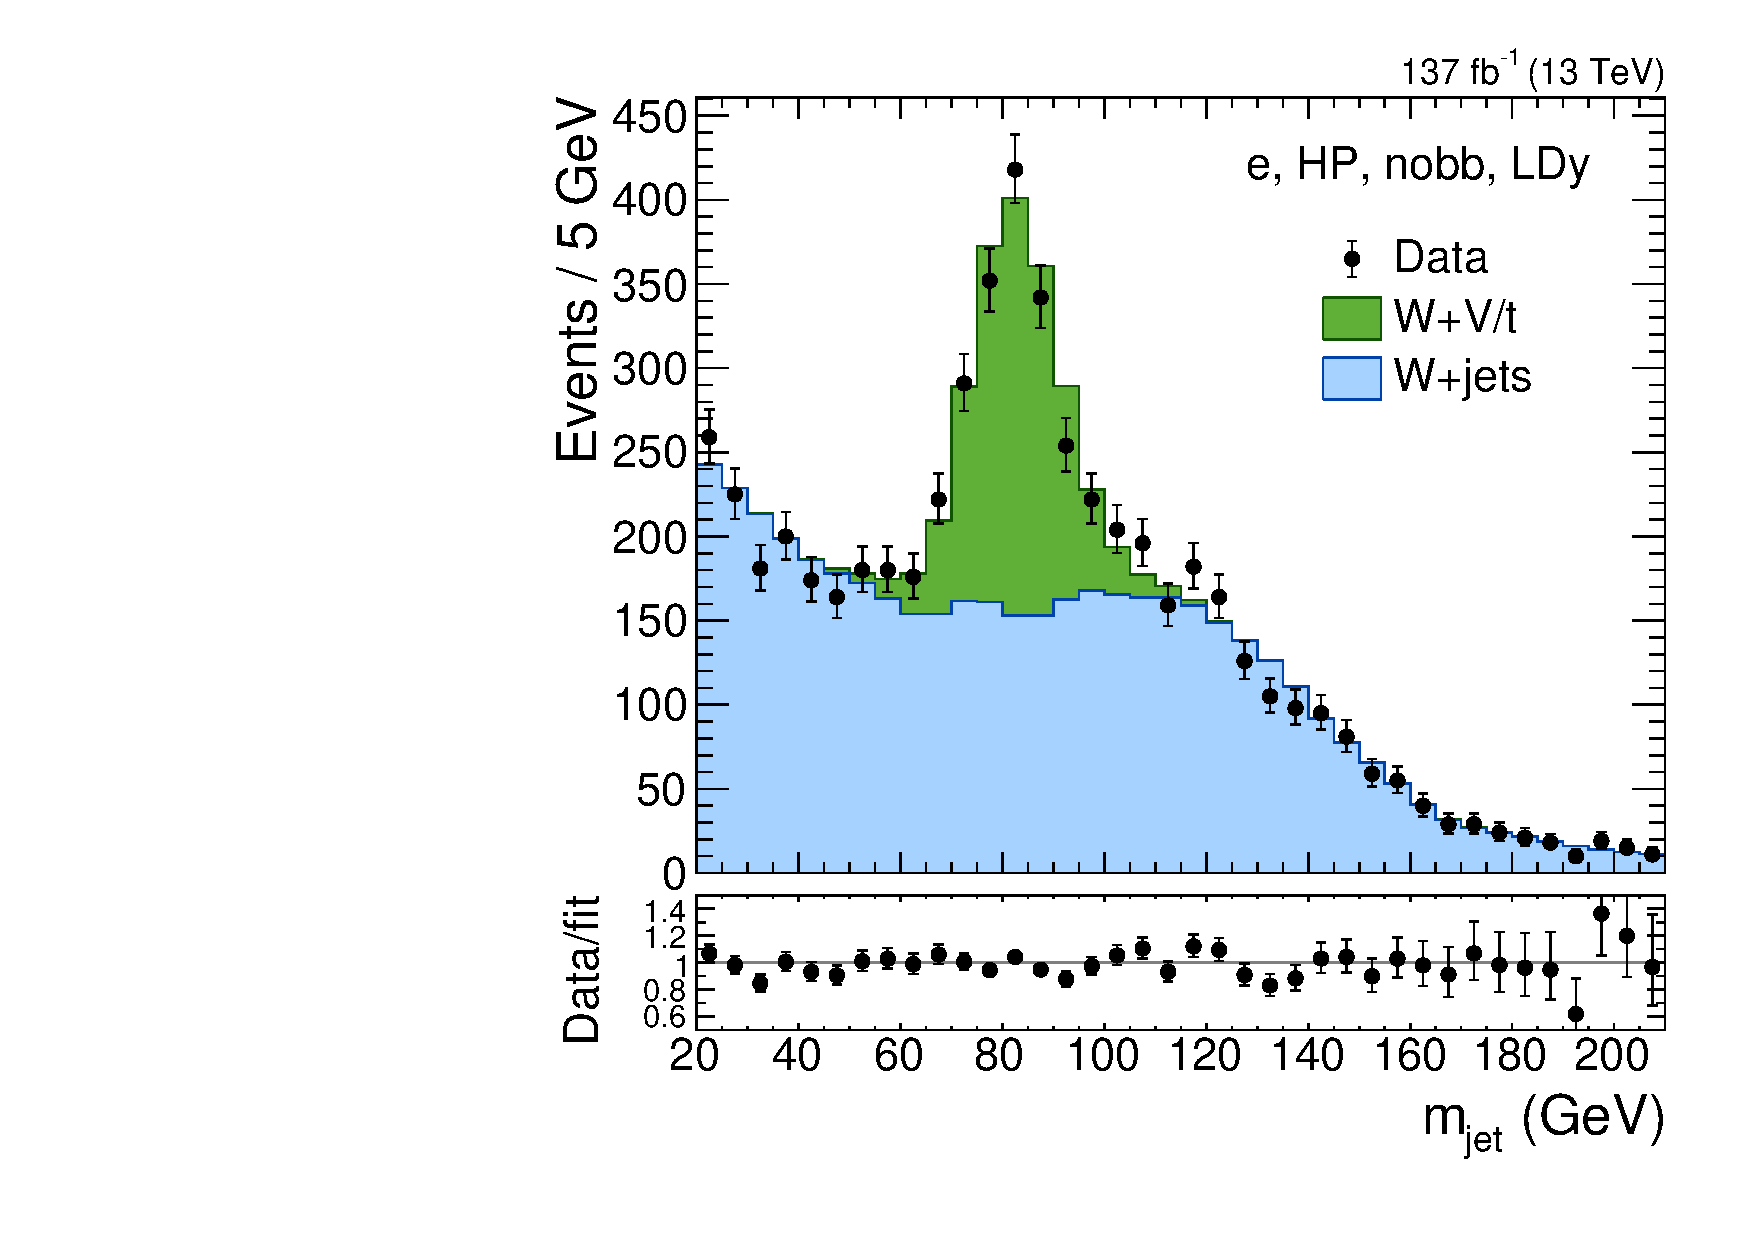
\includegraphics[width=0.18\textwidth]{fig/fitValidation/PostFit_SR_MJJ__e_HP_nobb_LDy_Run2.pdf}
  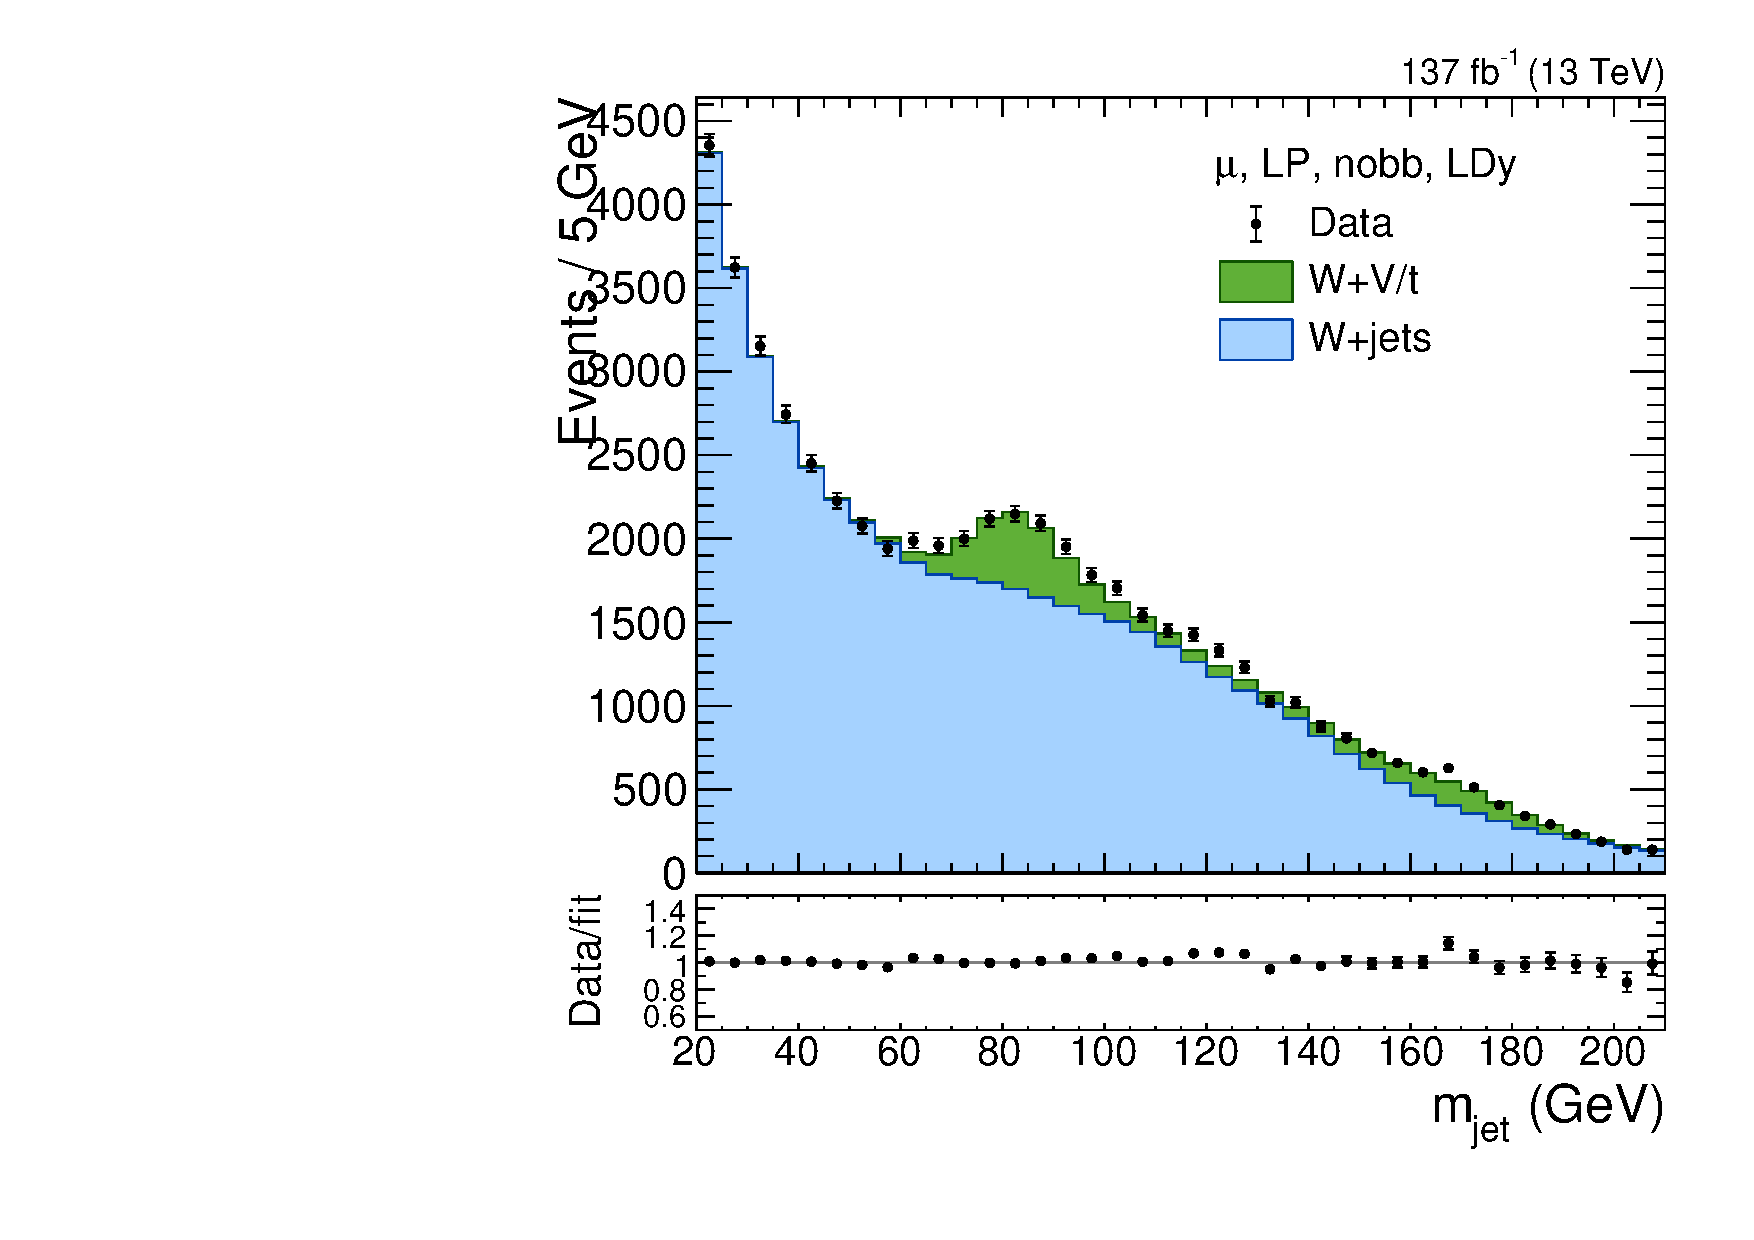
\includegraphics[width=0.18\textwidth]{fig/fitValidation/PostFit_SR_MJJ__mu_LP_nobb_LDy_Run2.pdf}
  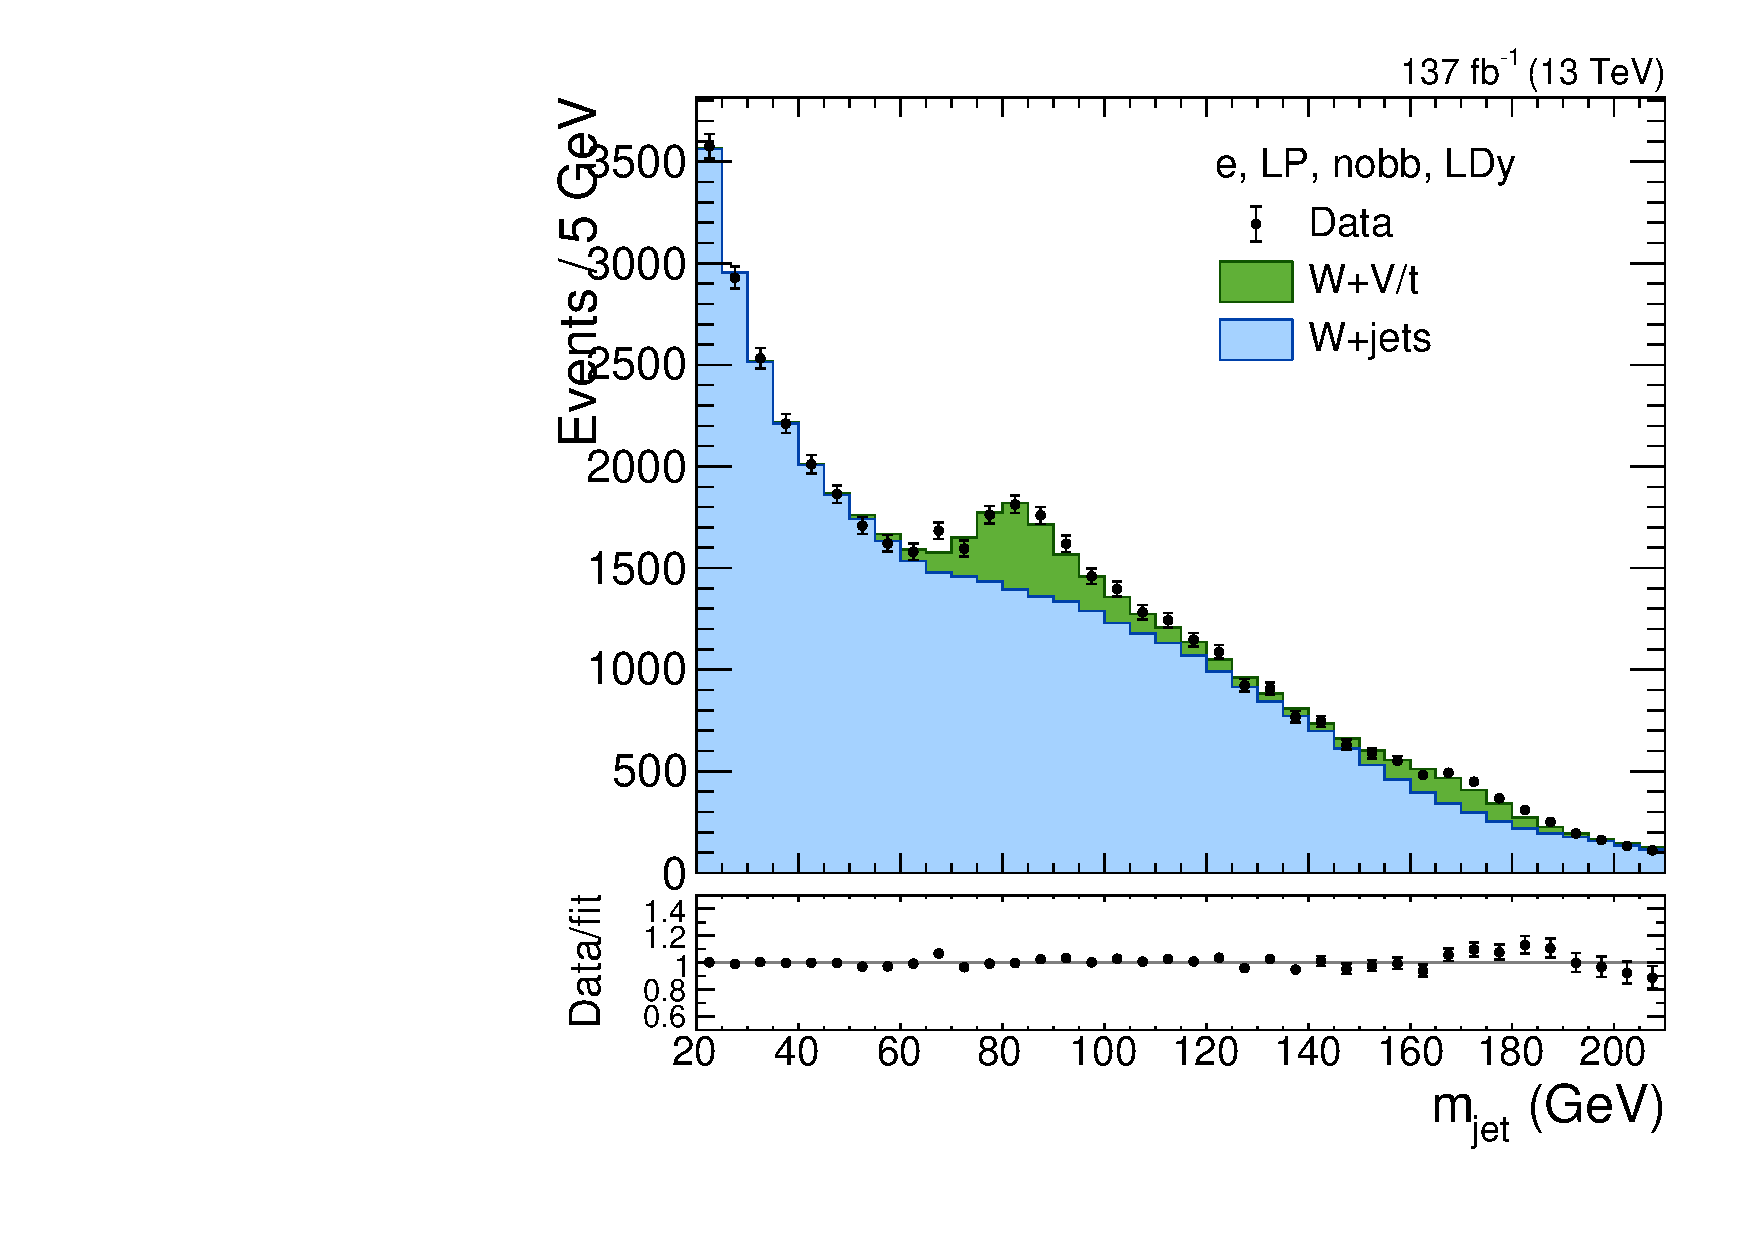
\includegraphics[width=0.18\textwidth]{fig/fitValidation/PostFit_SR_MJJ__e_LP_nobb_LDy_Run2.pdf}\\
  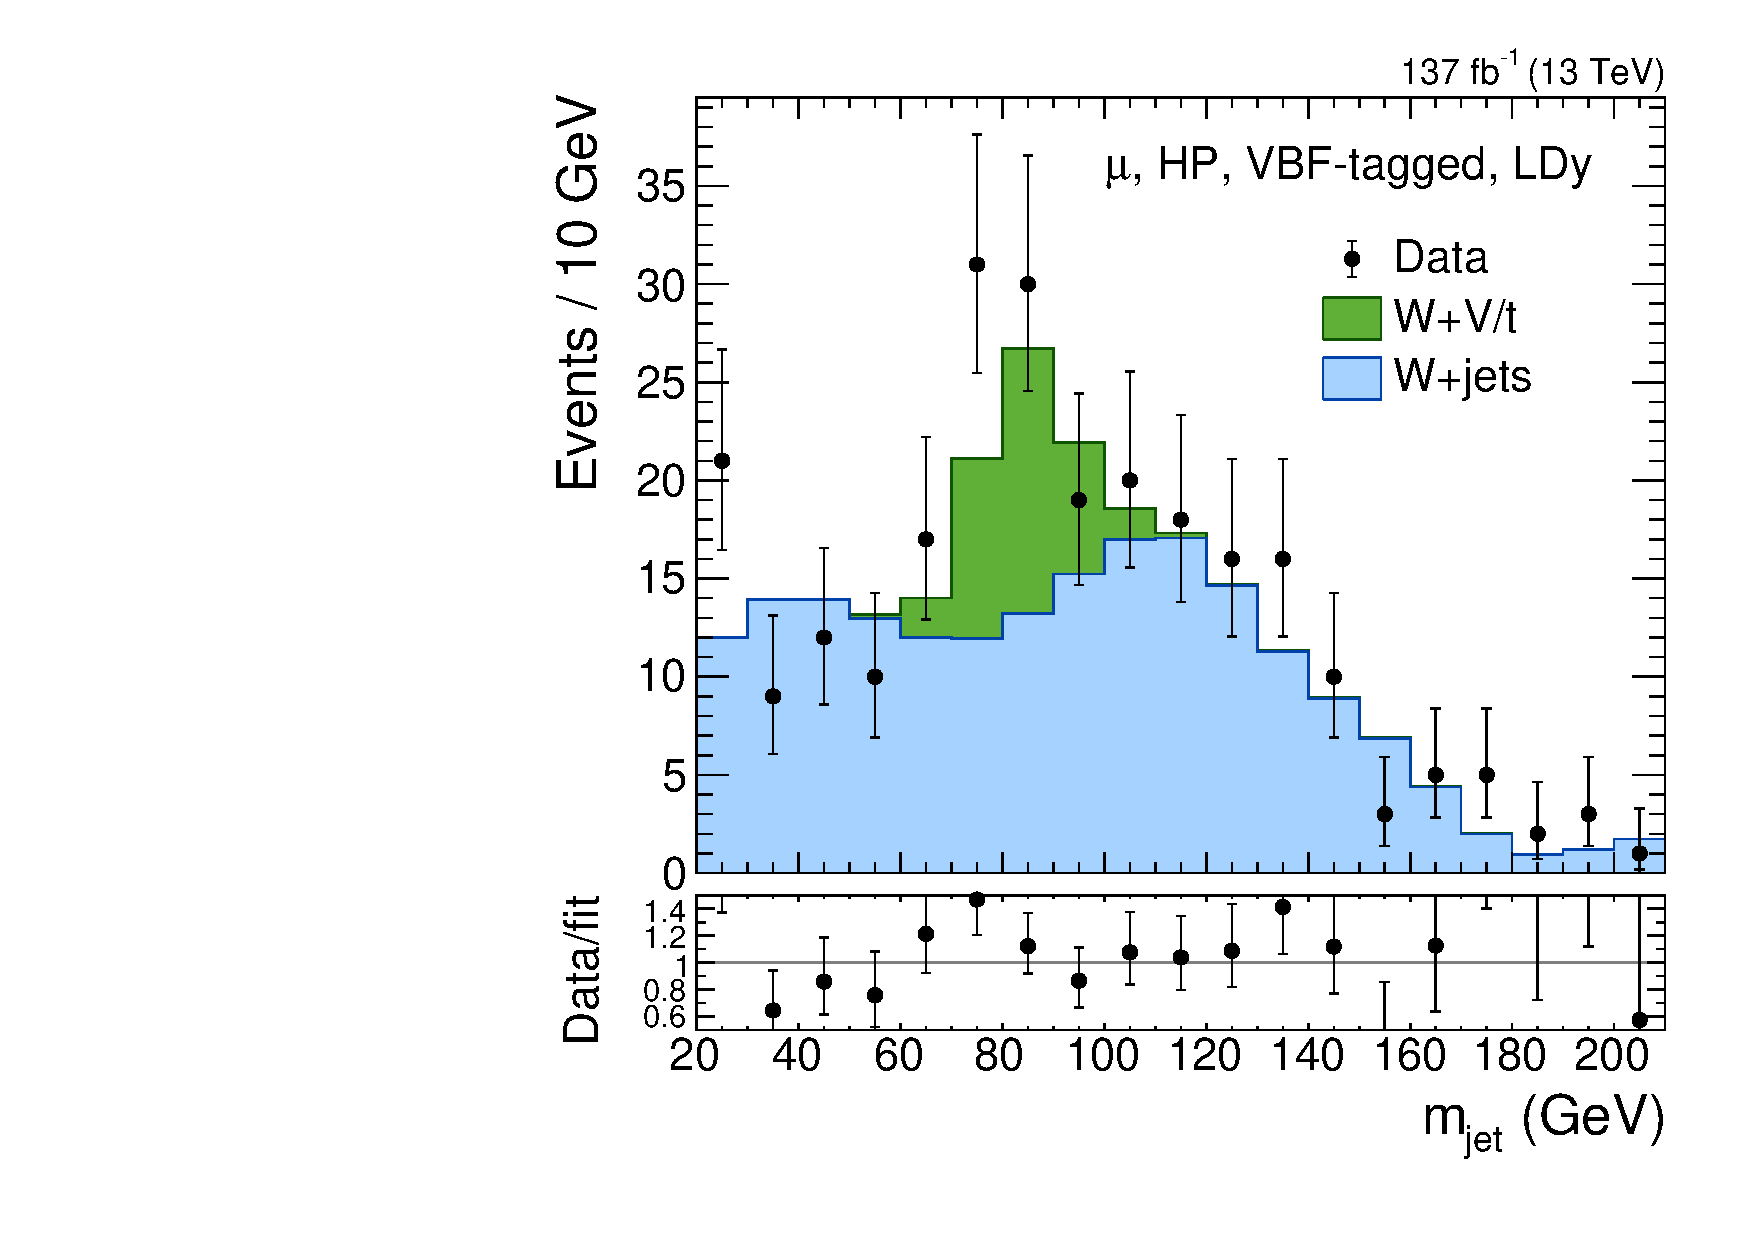
\includegraphics[width=0.18\textwidth]{fig/fitValidation/PostFit_SR_MJJ__mu_HP_vbf_LDy_Run2.pdf}
  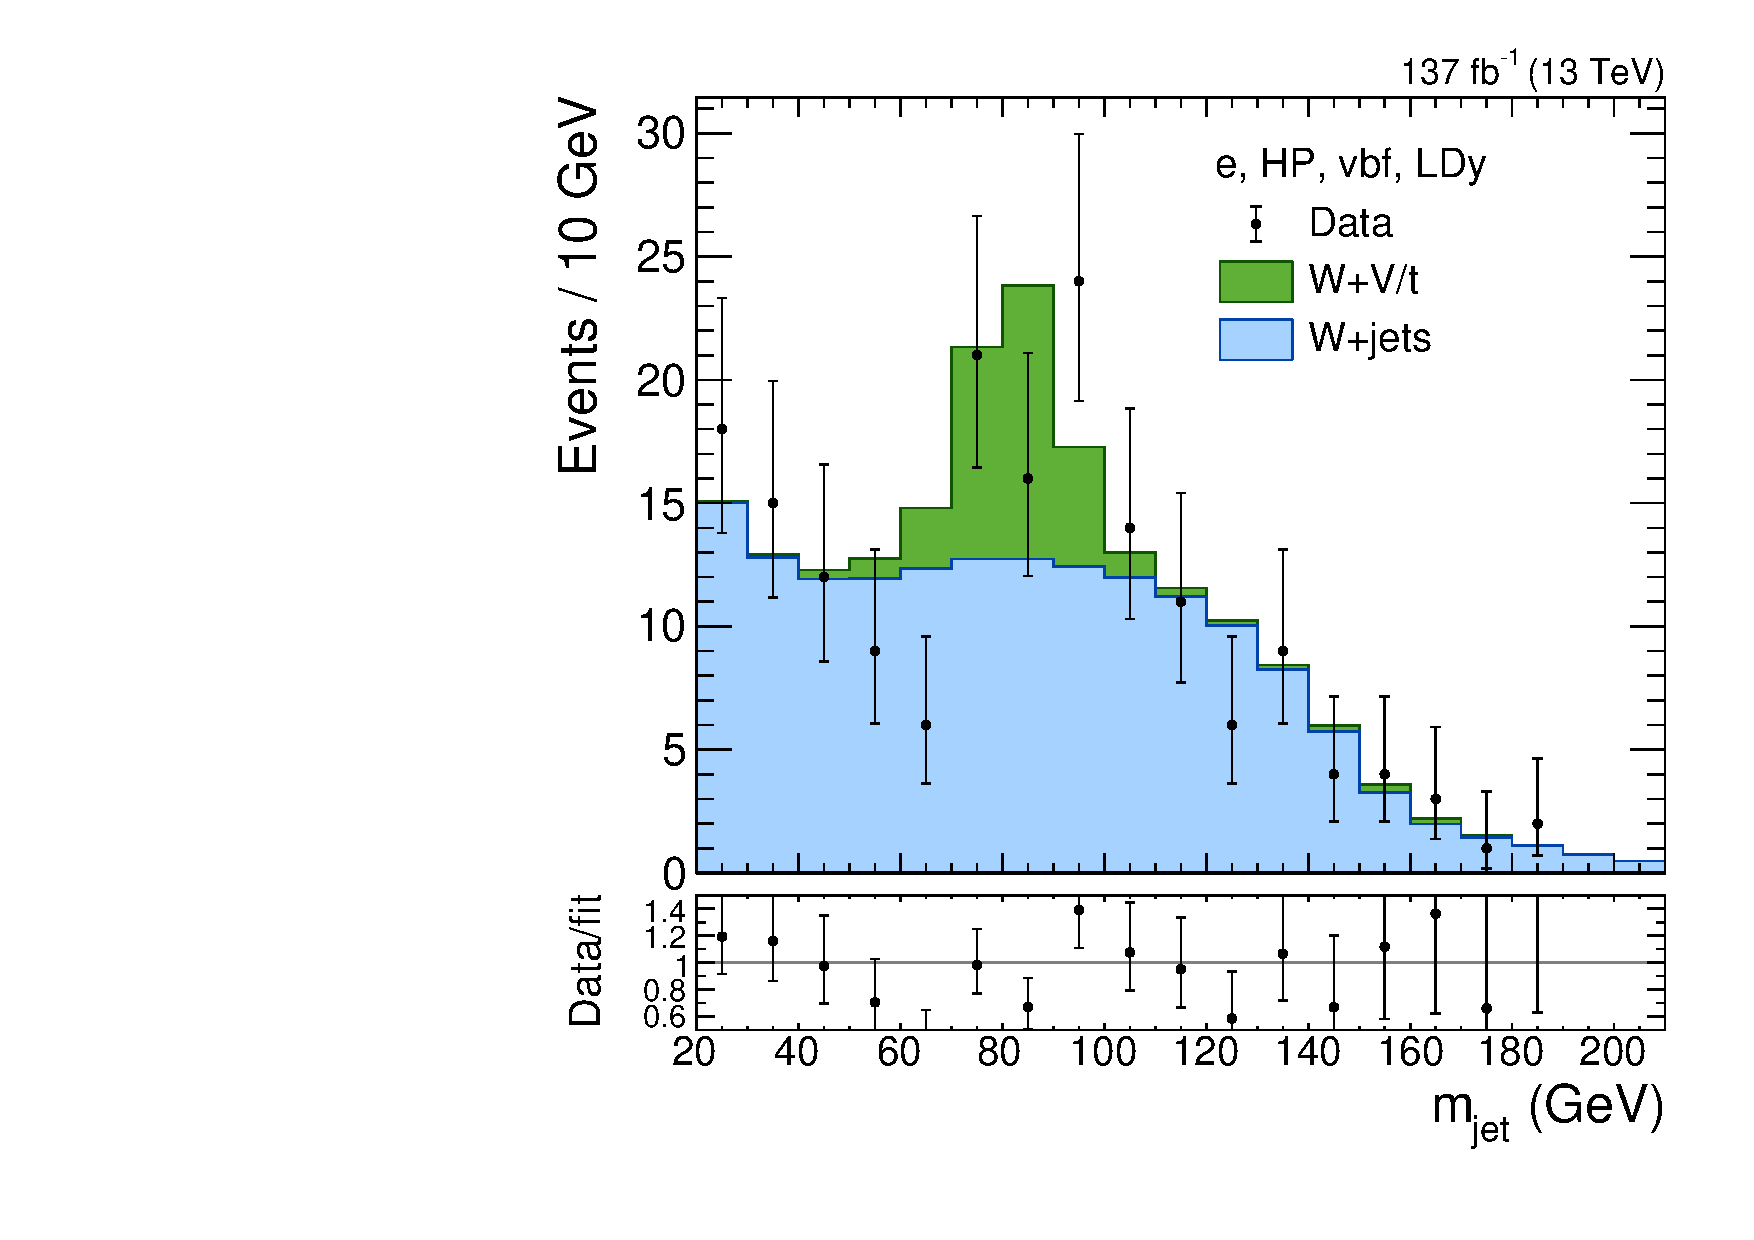
\includegraphics[width=0.18\textwidth]{fig/fitValidation/PostFit_SR_MJJ__e_HP_vbf_LDy_Run2.pdf}
  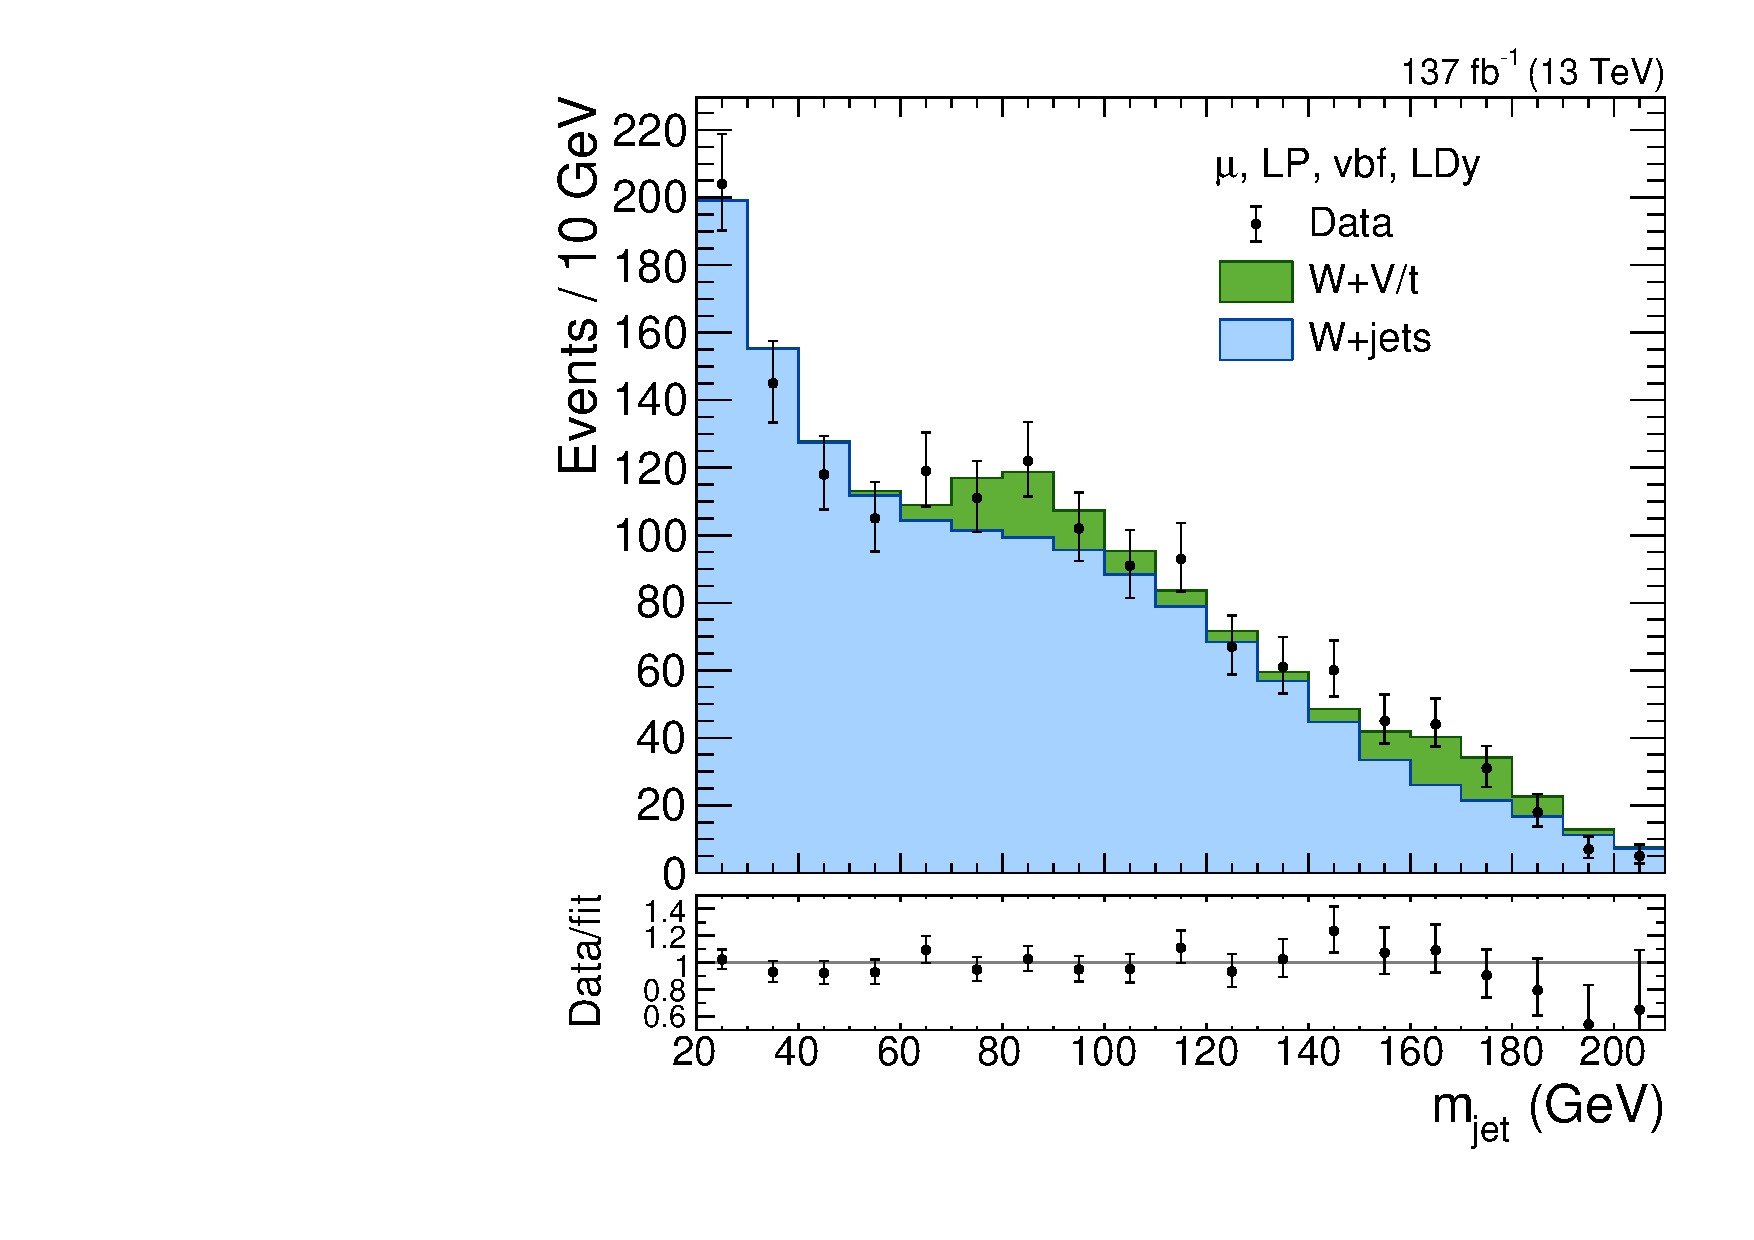
\includegraphics[width=0.18\textwidth]{fig/fitValidation/PostFit_SR_MJJ__mu_LP_vbf_LDy_Run2.pdf}
  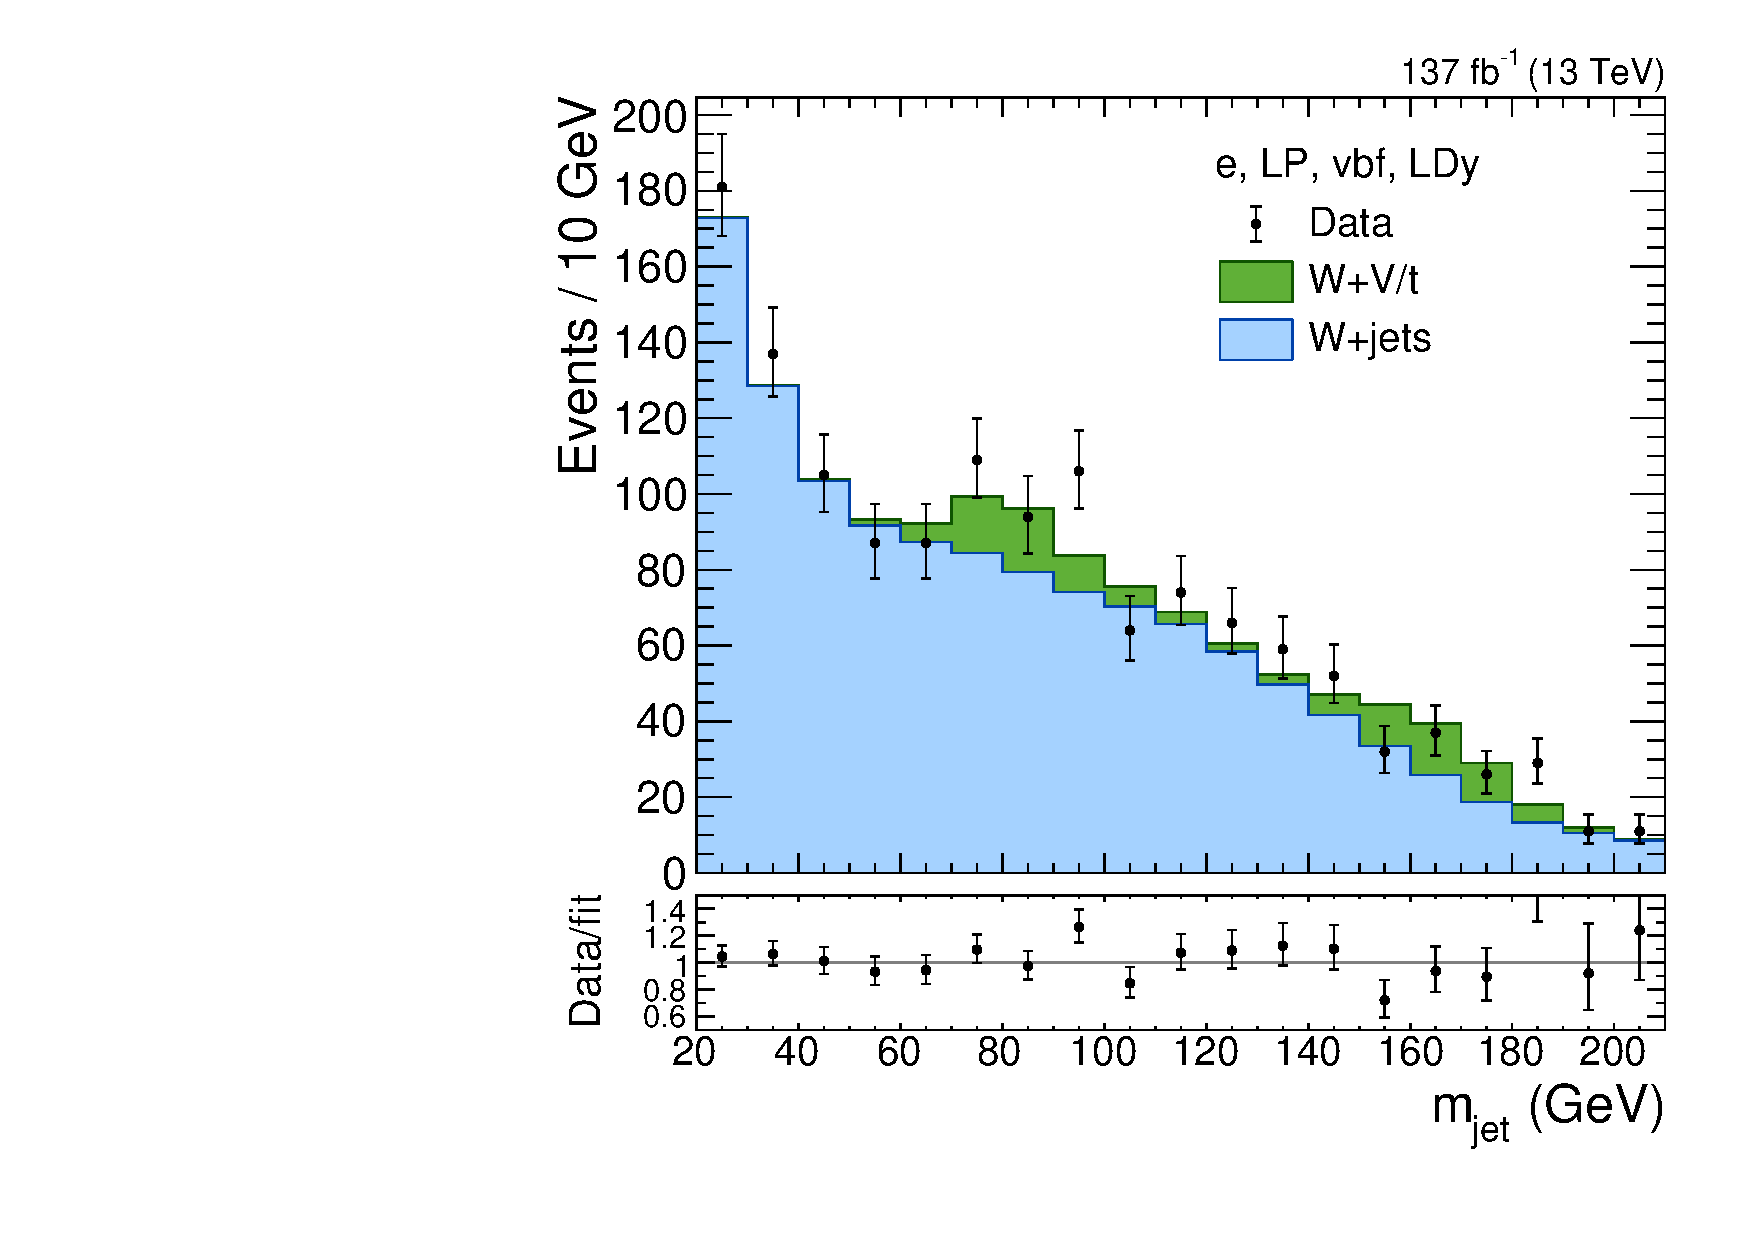
\includegraphics[width=0.18\textwidth]{fig/fitValidation/PostFit_SR_MJJ__e_LP_vbf_LDy_Run2.pdf}\\
  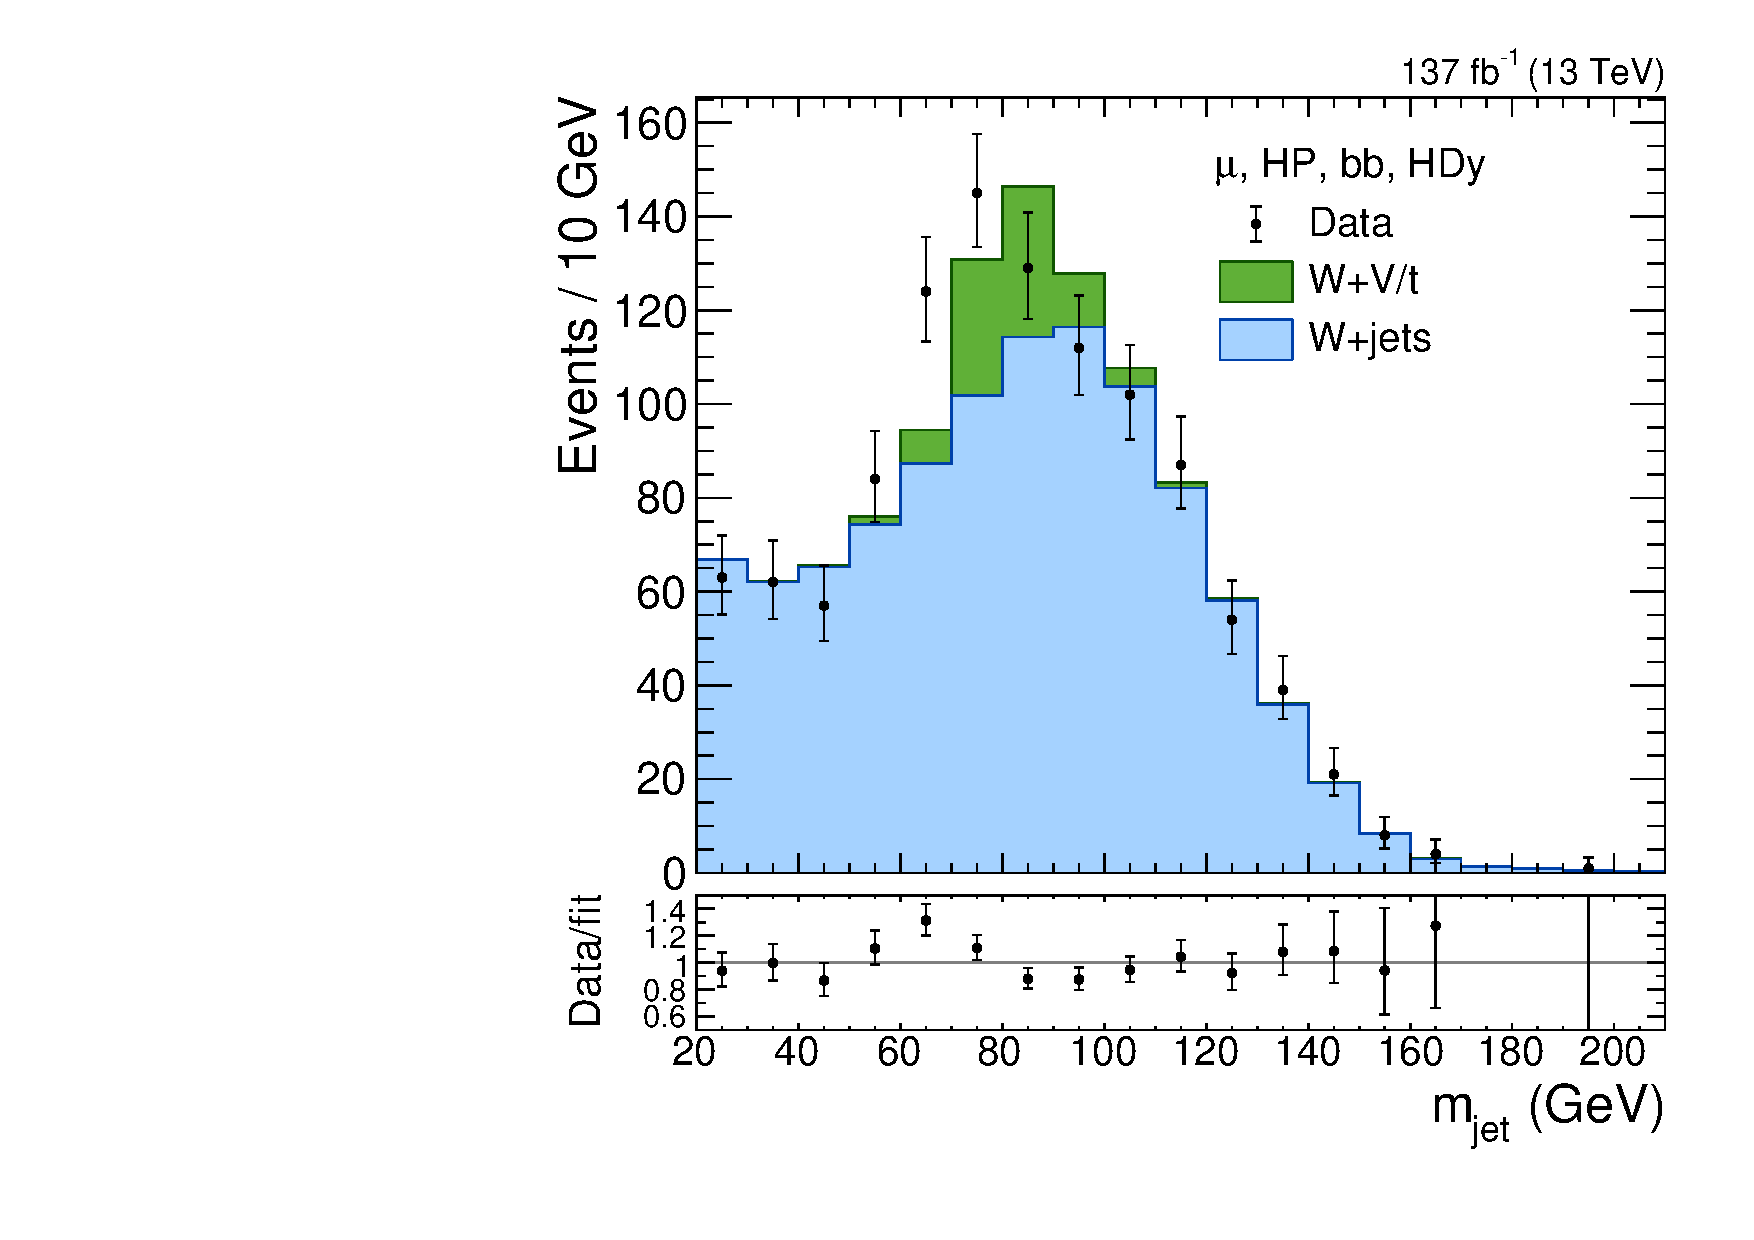
\includegraphics[width=0.18\textwidth]{fig/fitValidation/PostFit_SR_MJJ__mu_HP_bb_HDy_Run2.pdf}
  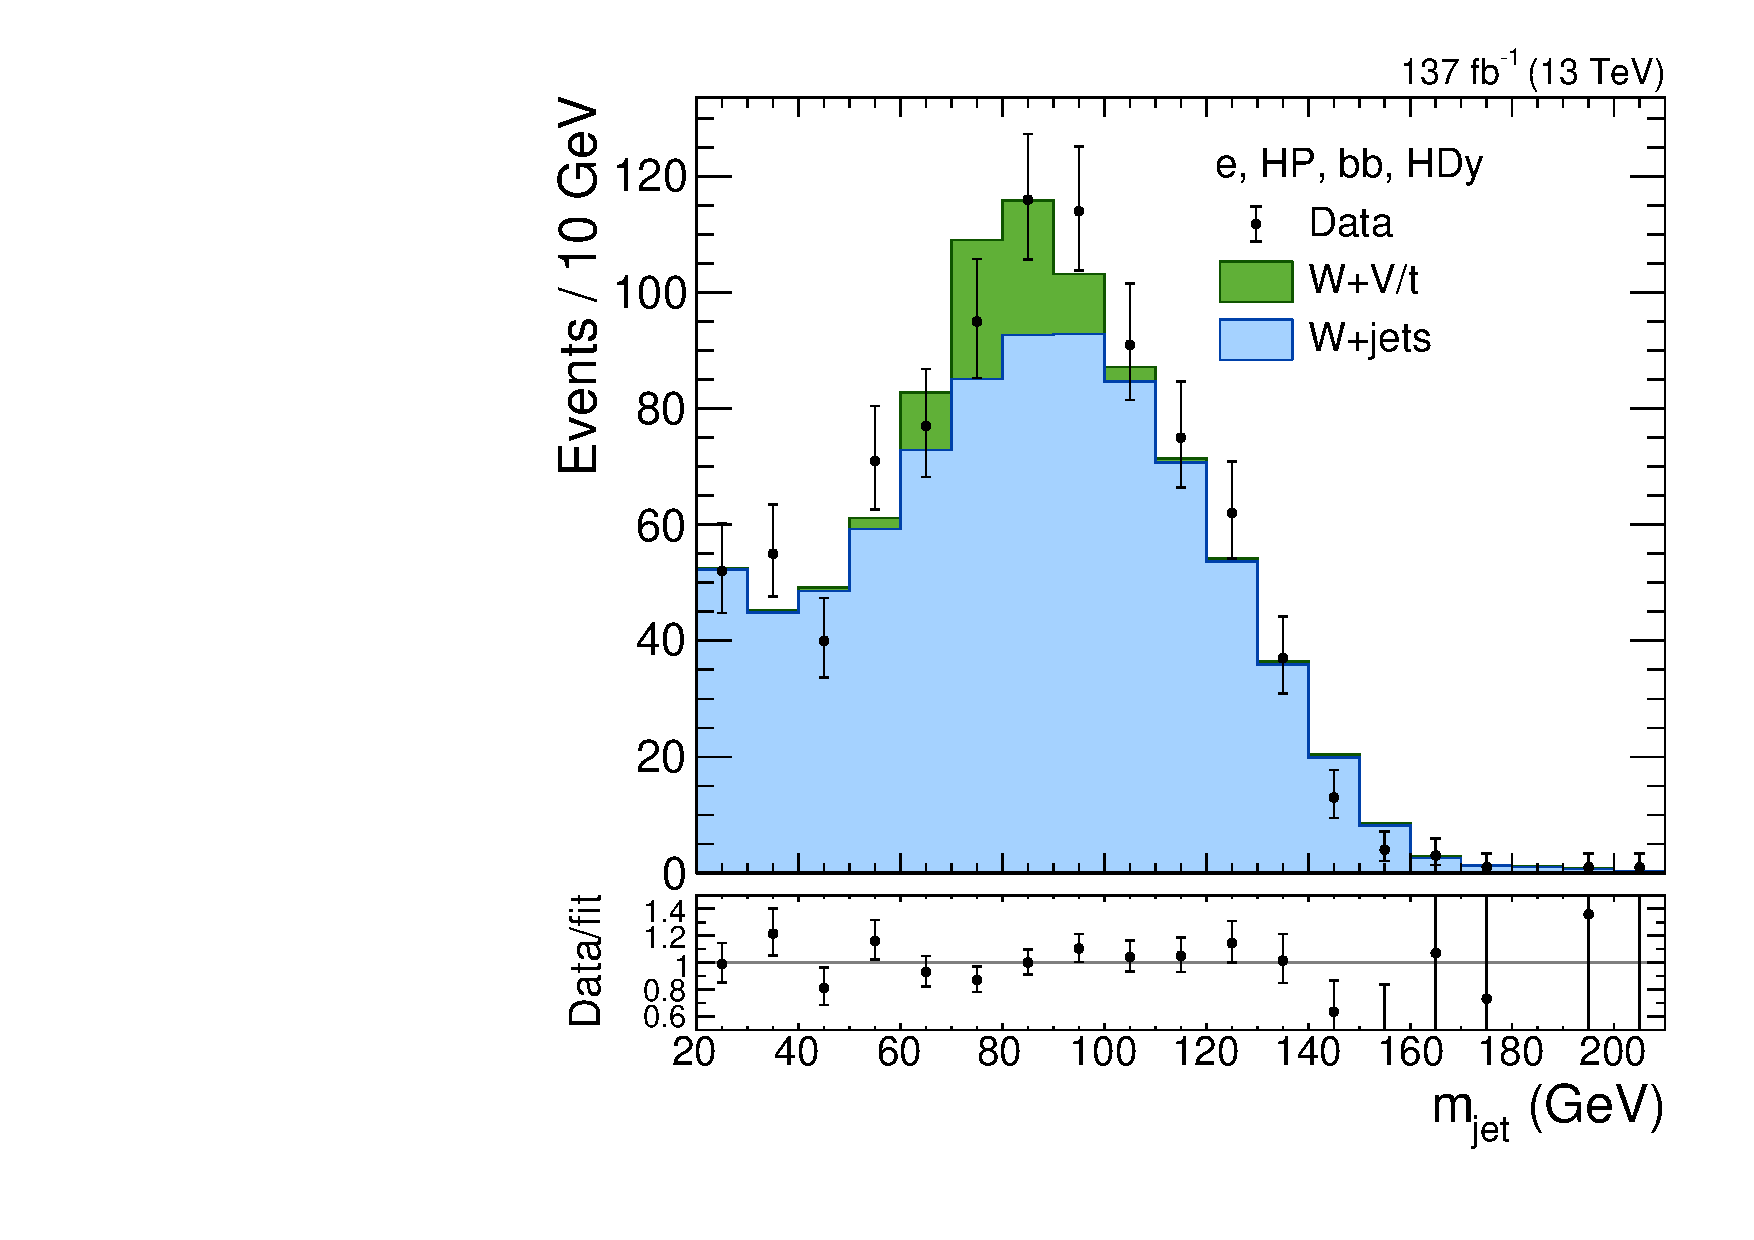
\includegraphics[width=0.18\textwidth]{fig/fitValidation/PostFit_SR_MJJ__e_HP_bb_HDy_Run2.pdf}
  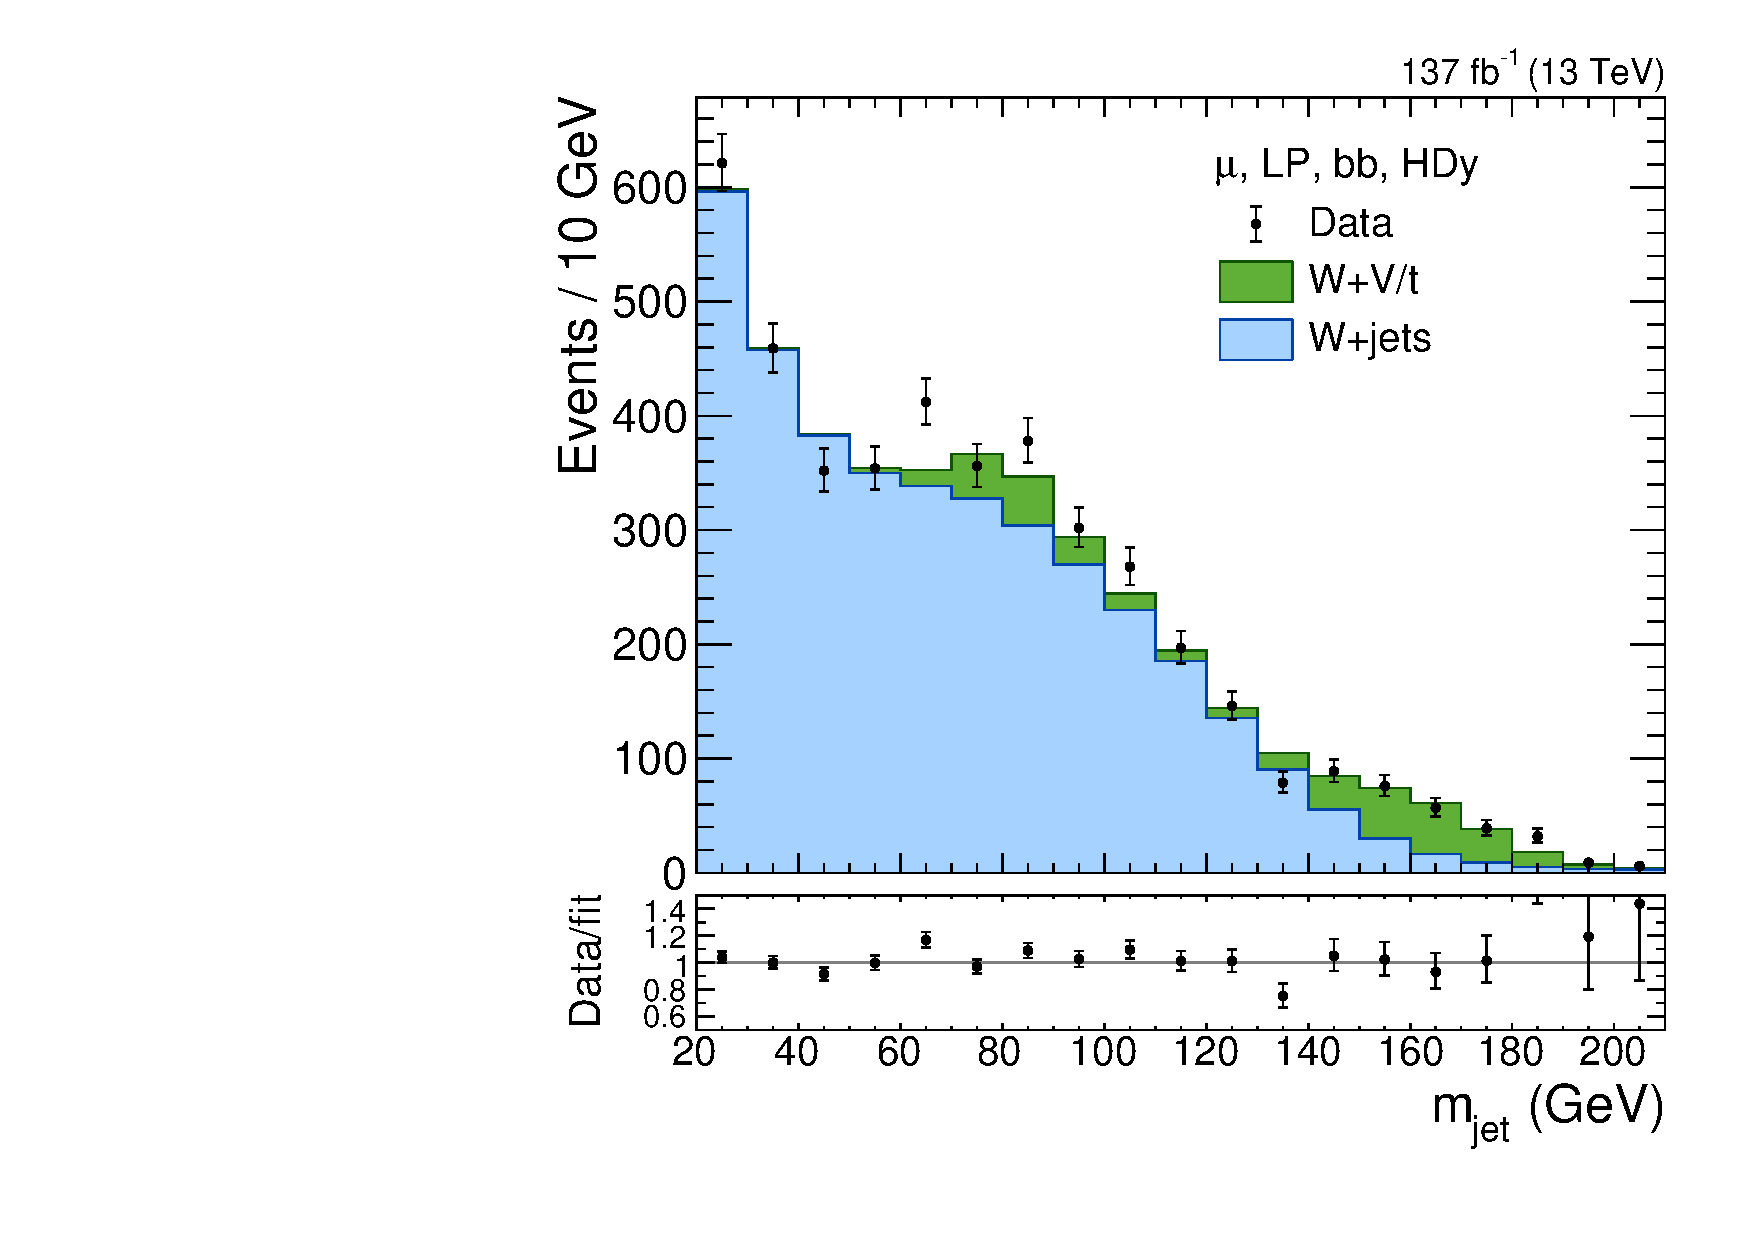
\includegraphics[width=0.18\textwidth]{fig/fitValidation/PostFit_SR_MJJ__mu_LP_bb_HDy_Run2.pdf}
  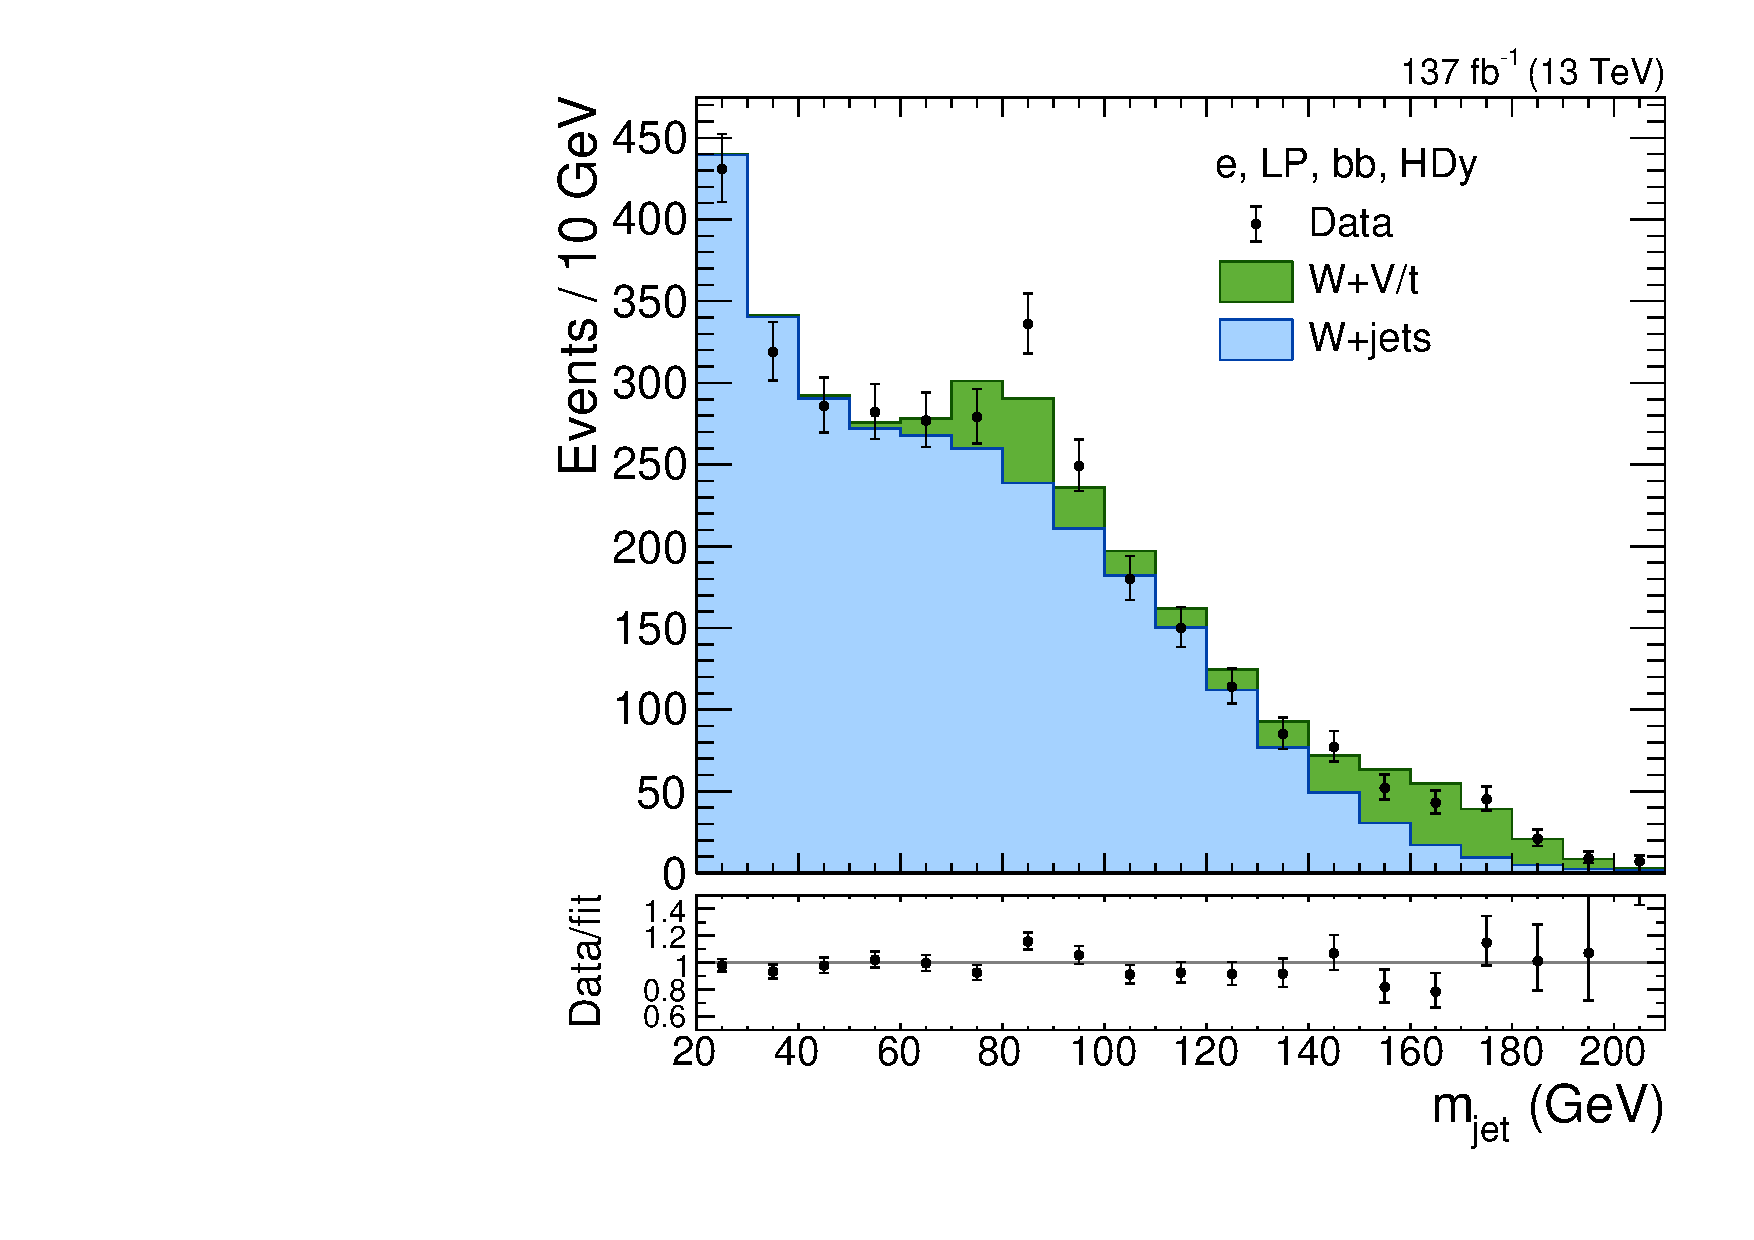
\includegraphics[width=0.18\textwidth]{fig/fitValidation/PostFit_SR_MJJ__e_LP_bb_HDy_Run2.pdf}\\
  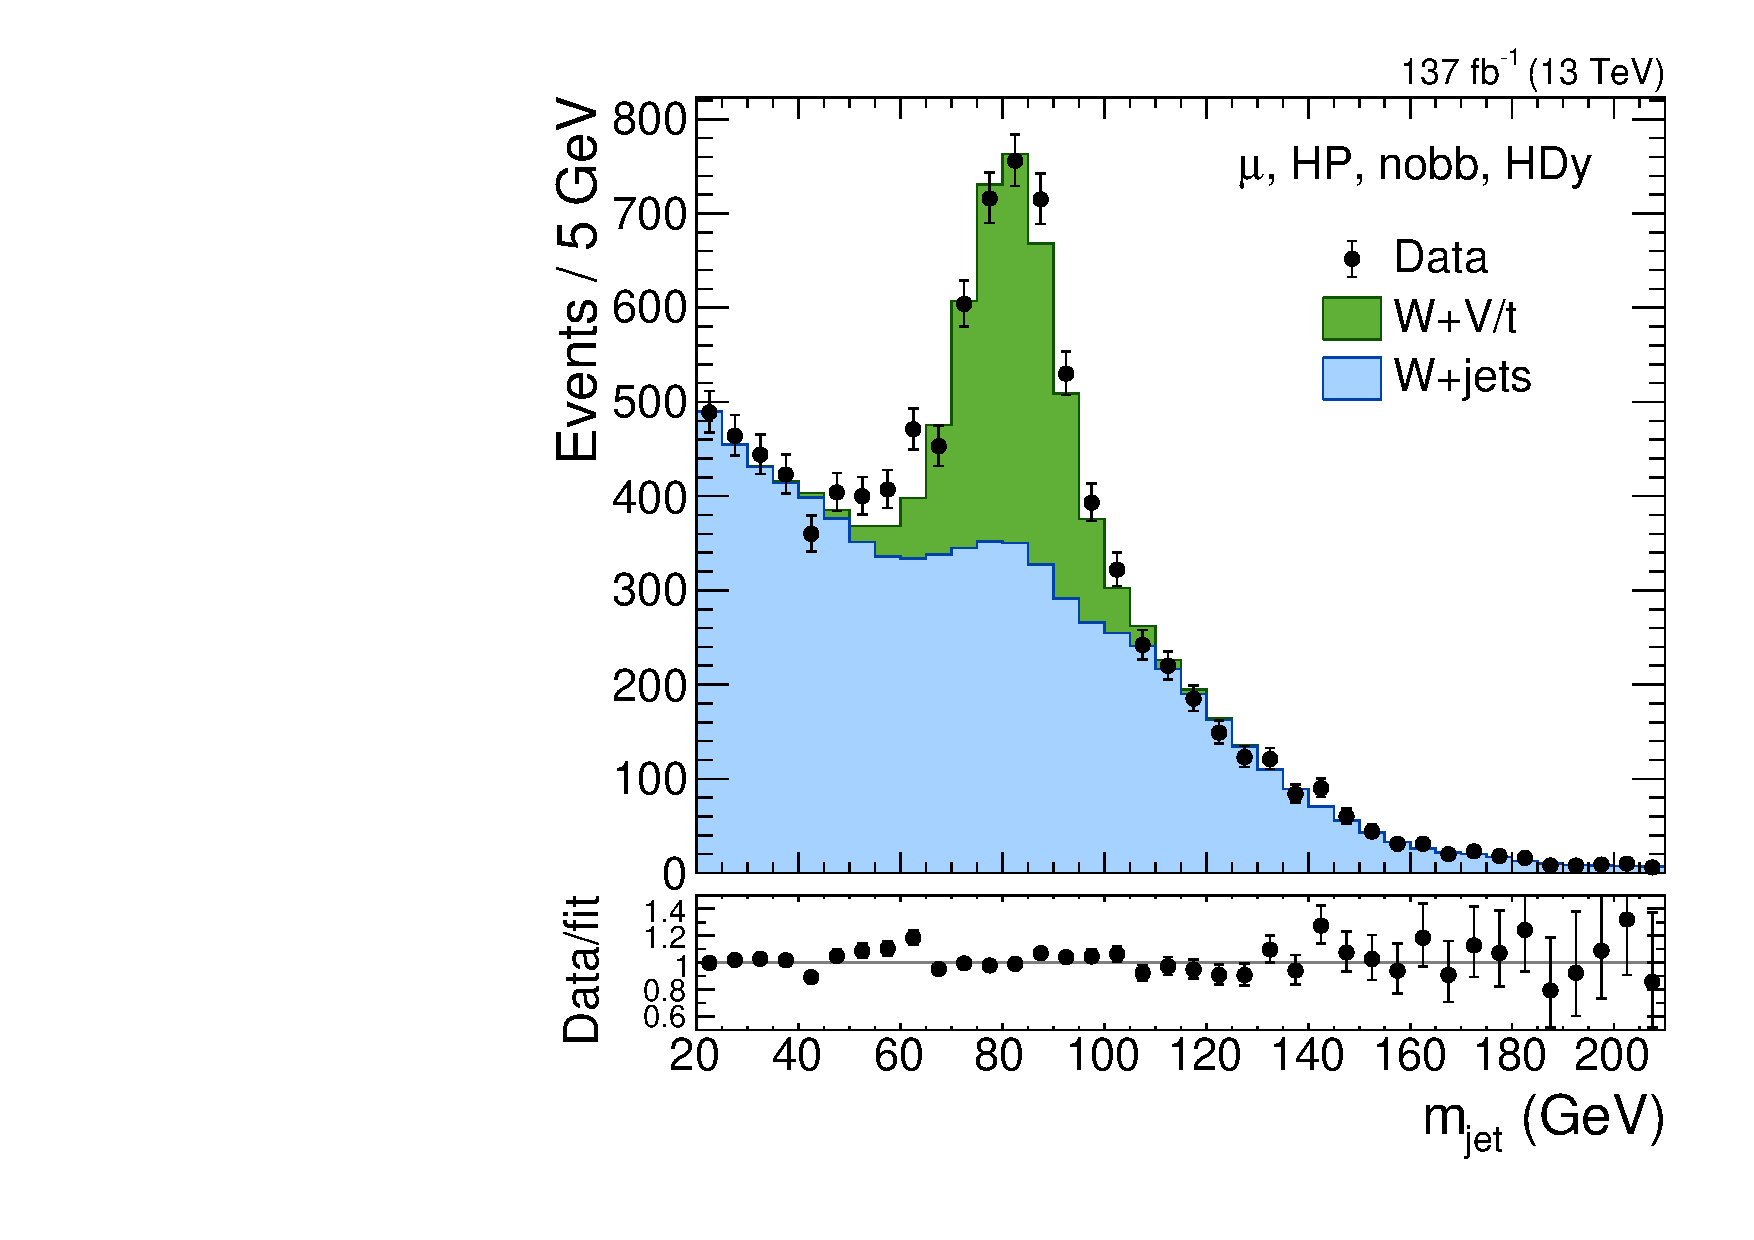
\includegraphics[width=0.18\textwidth]{fig/fitValidation/PostFit_SR_MJJ__mu_HP_nobb_HDy_Run2.pdf}
  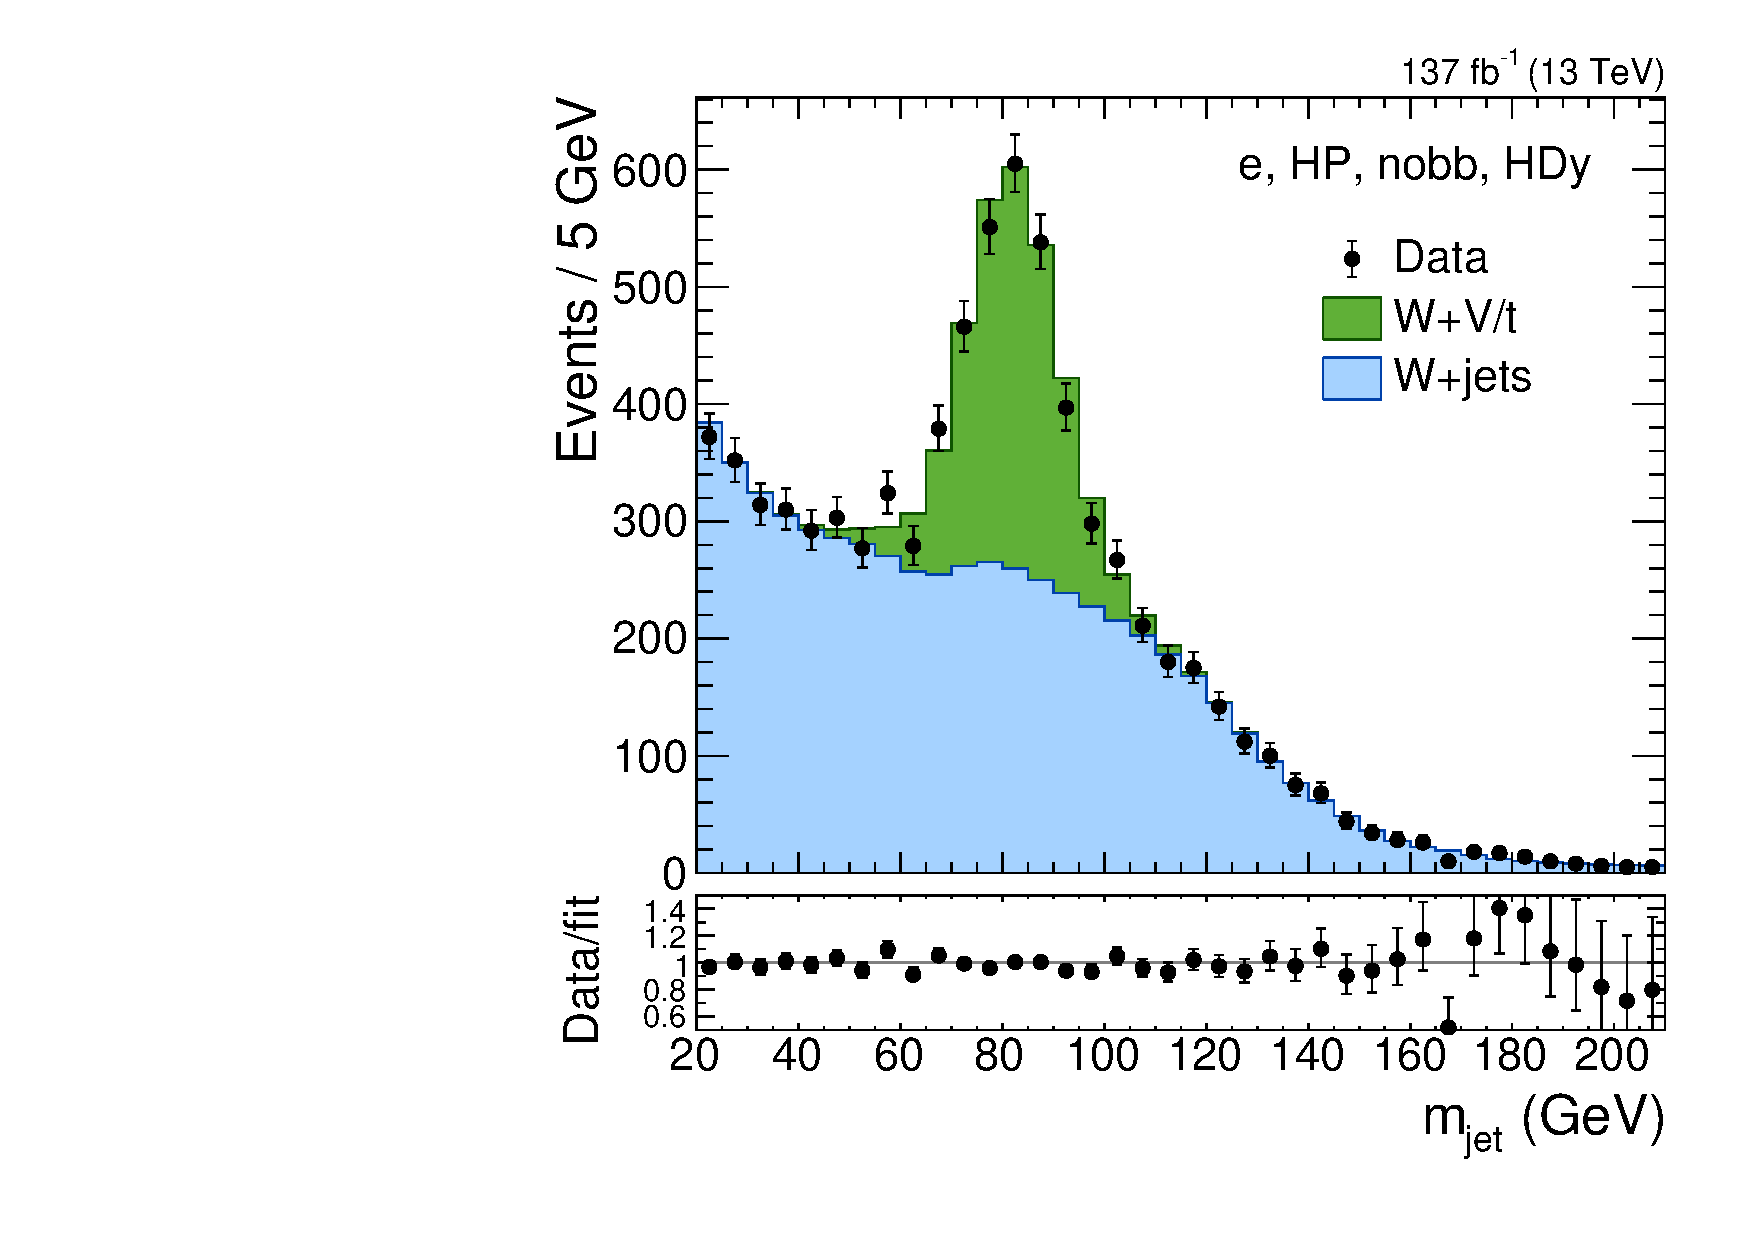
\includegraphics[width=0.18\textwidth]{fig/fitValidation/PostFit_SR_MJJ__e_HP_nobb_HDy_Run2.pdf}
  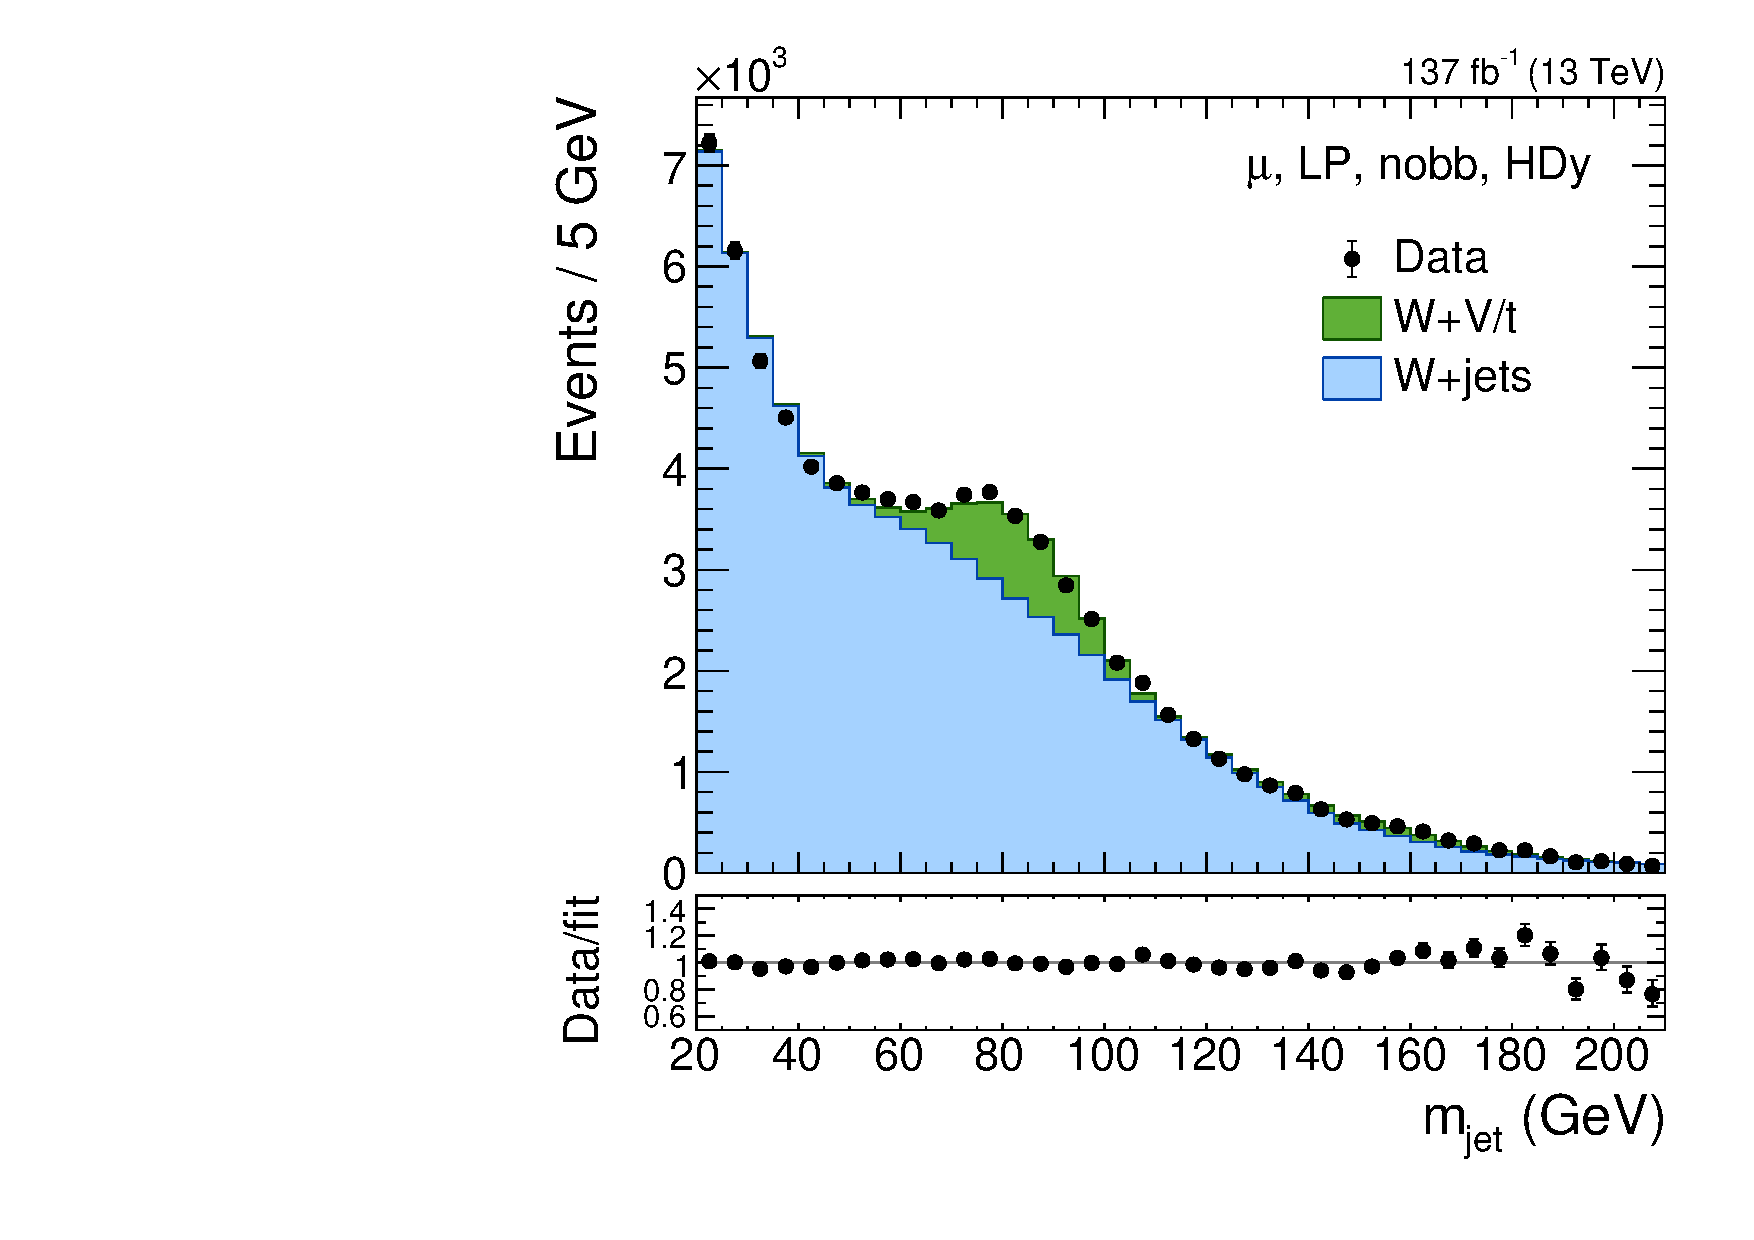
\includegraphics[width=0.18\textwidth]{fig/fitValidation/PostFit_SR_MJJ__mu_LP_nobb_HDy_Run2.pdf}
  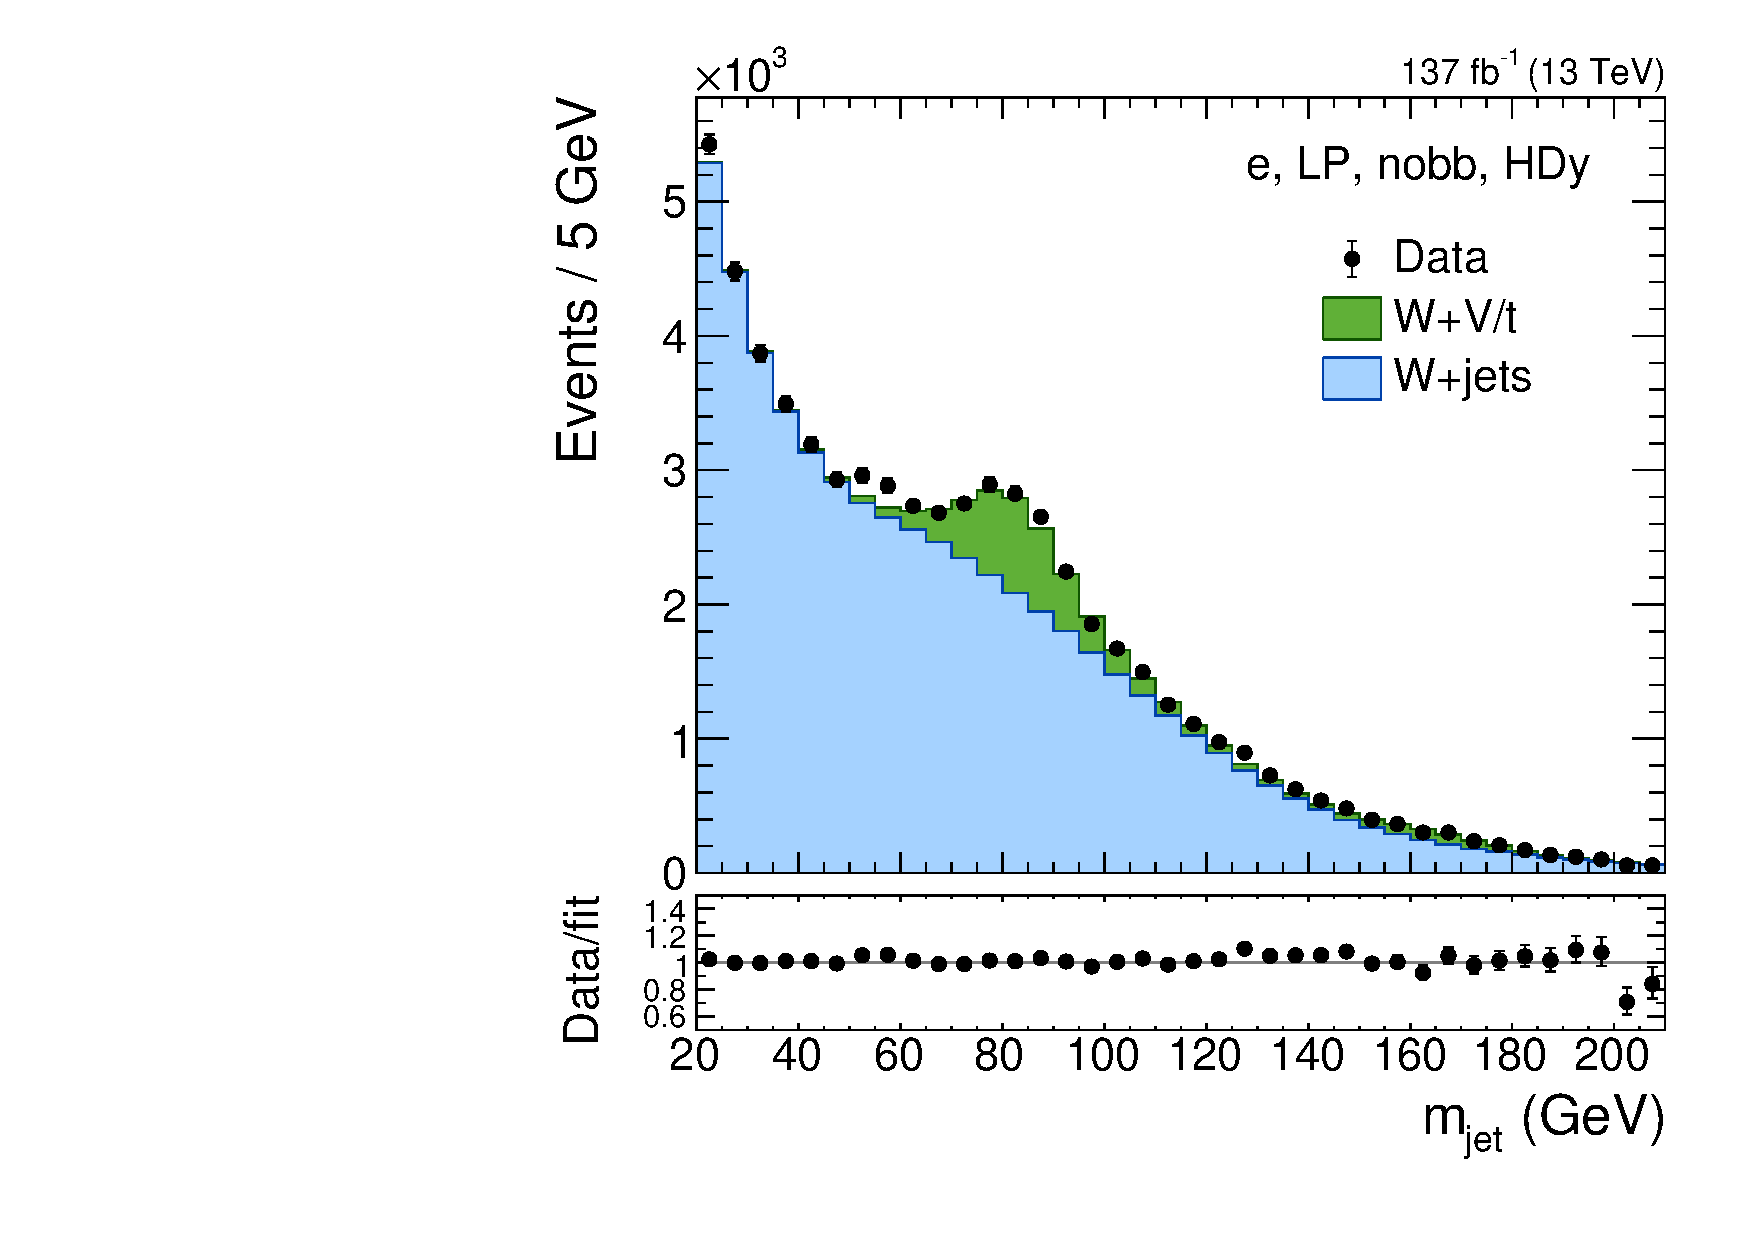
\includegraphics[width=0.18\textwidth]{fig/fitValidation/PostFit_SR_MJJ__e_LP_nobb_HDy_Run2.pdf}\\
  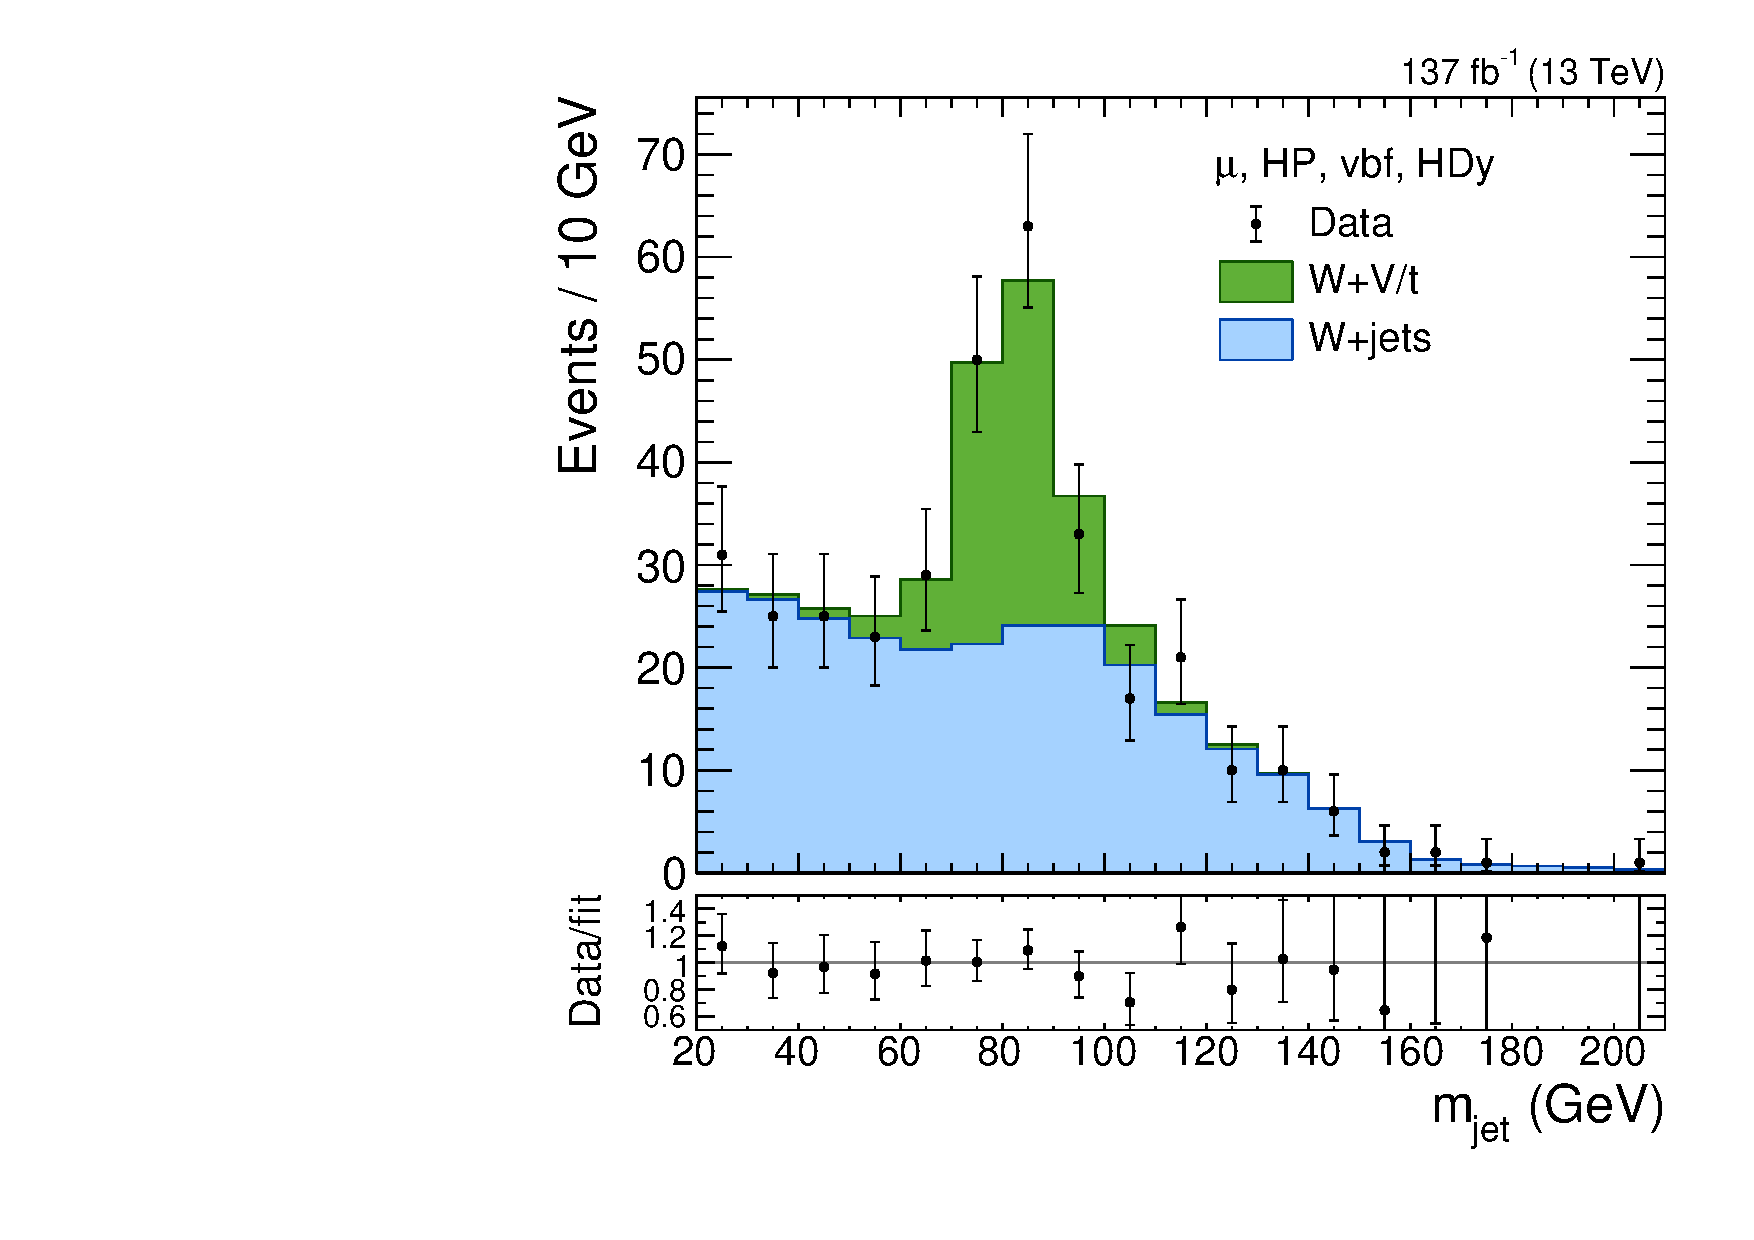
\includegraphics[width=0.18\textwidth]{fig/fitValidation/PostFit_SR_MJJ__mu_HP_vbf_HDy_Run2.pdf}
  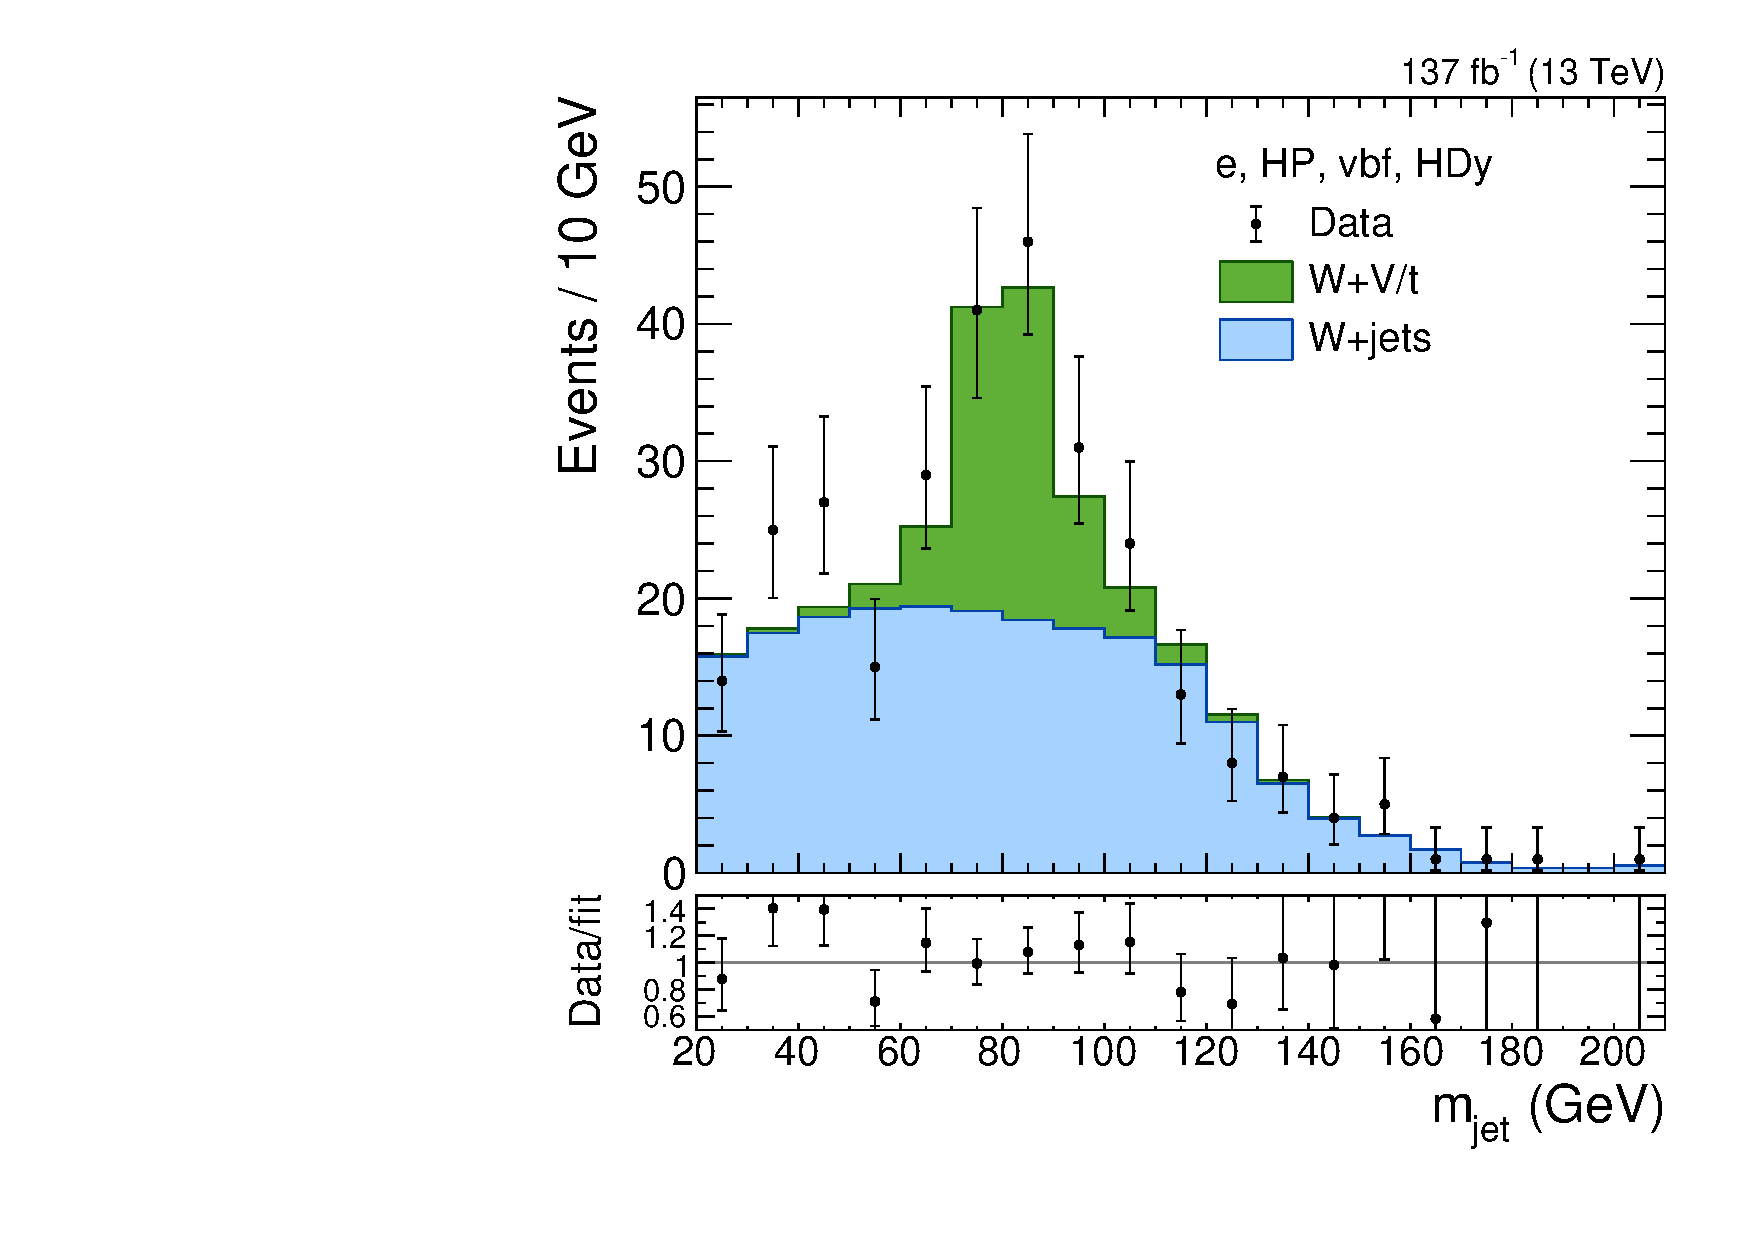
\includegraphics[width=0.18\textwidth]{fig/fitValidation/PostFit_SR_MJJ__e_HP_vbf_HDy_Run2.pdf}
  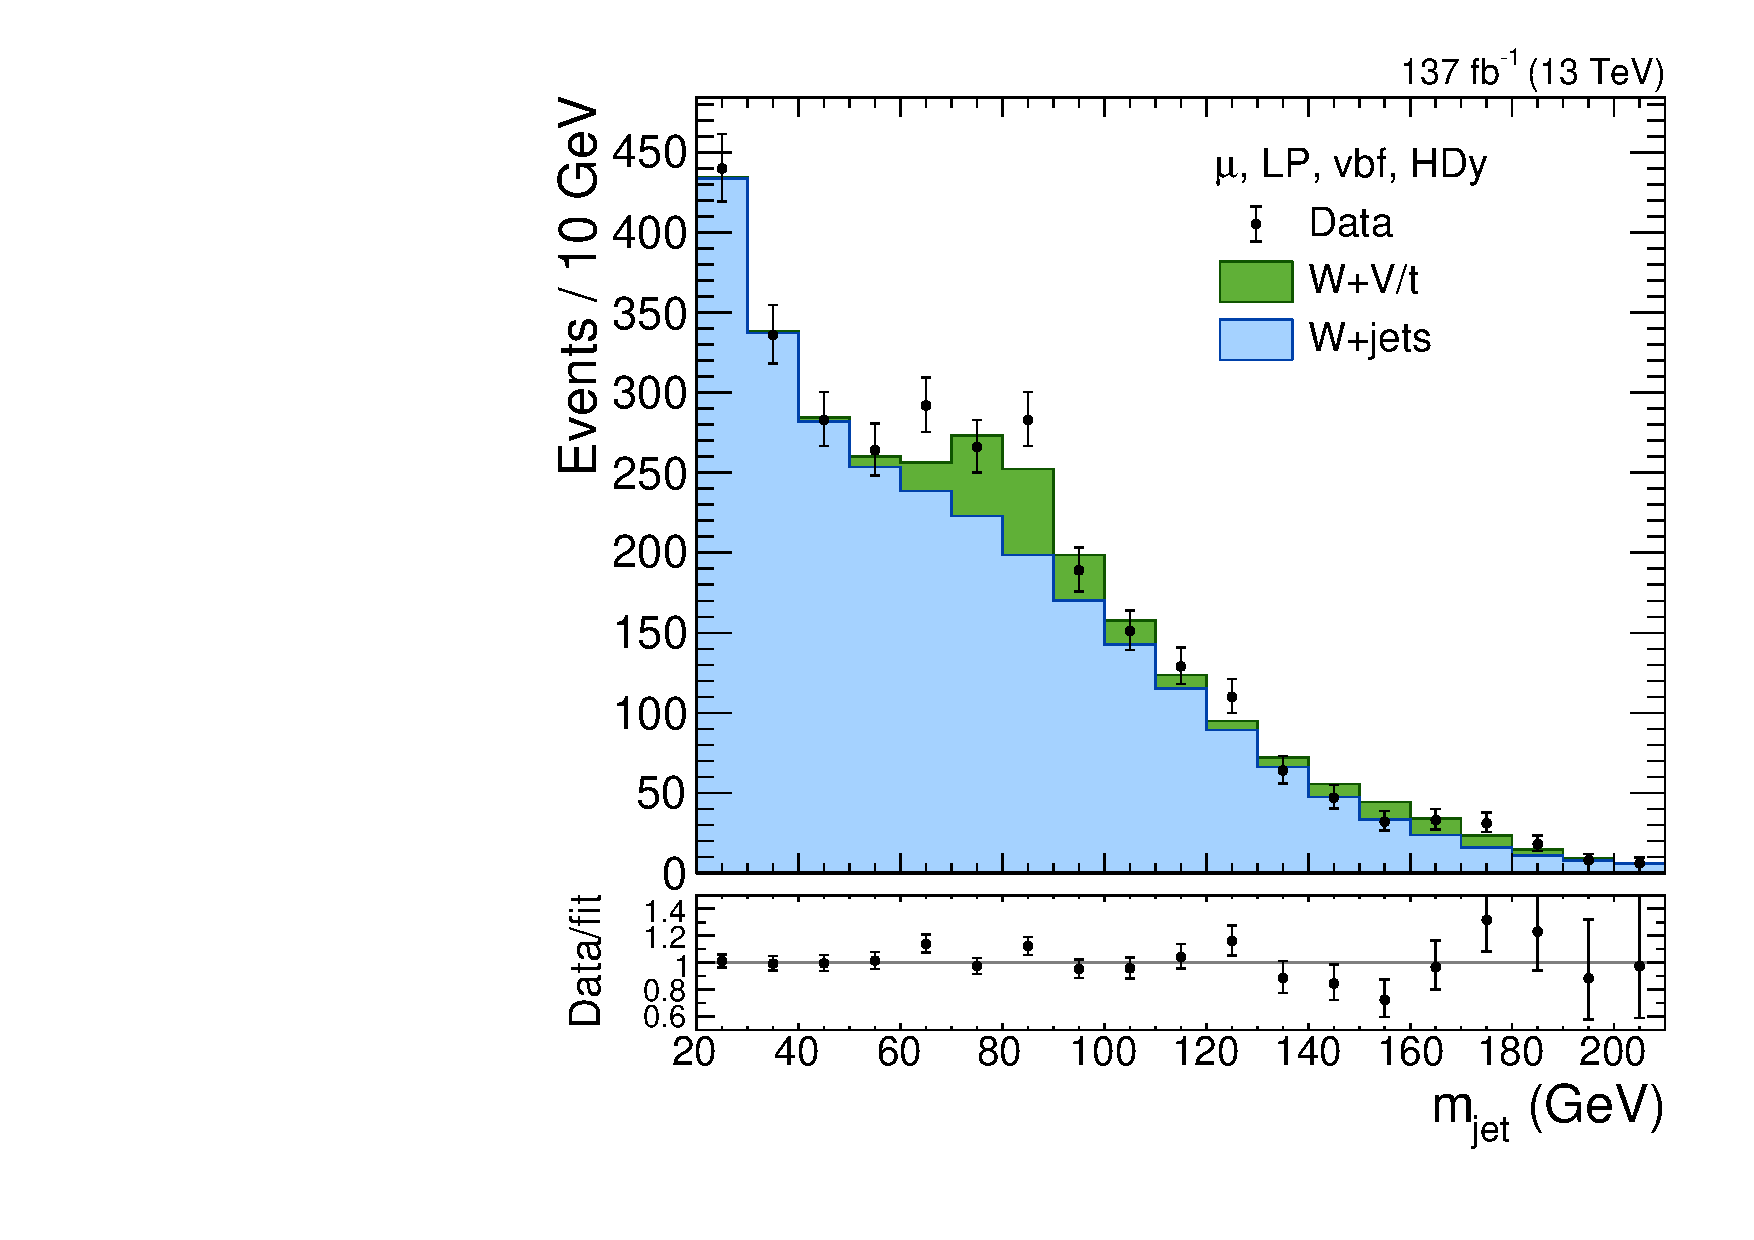
\includegraphics[width=0.18\textwidth]{fig/fitValidation/PostFit_SR_MJJ__mu_LP_vbf_HDy_Run2.pdf}
  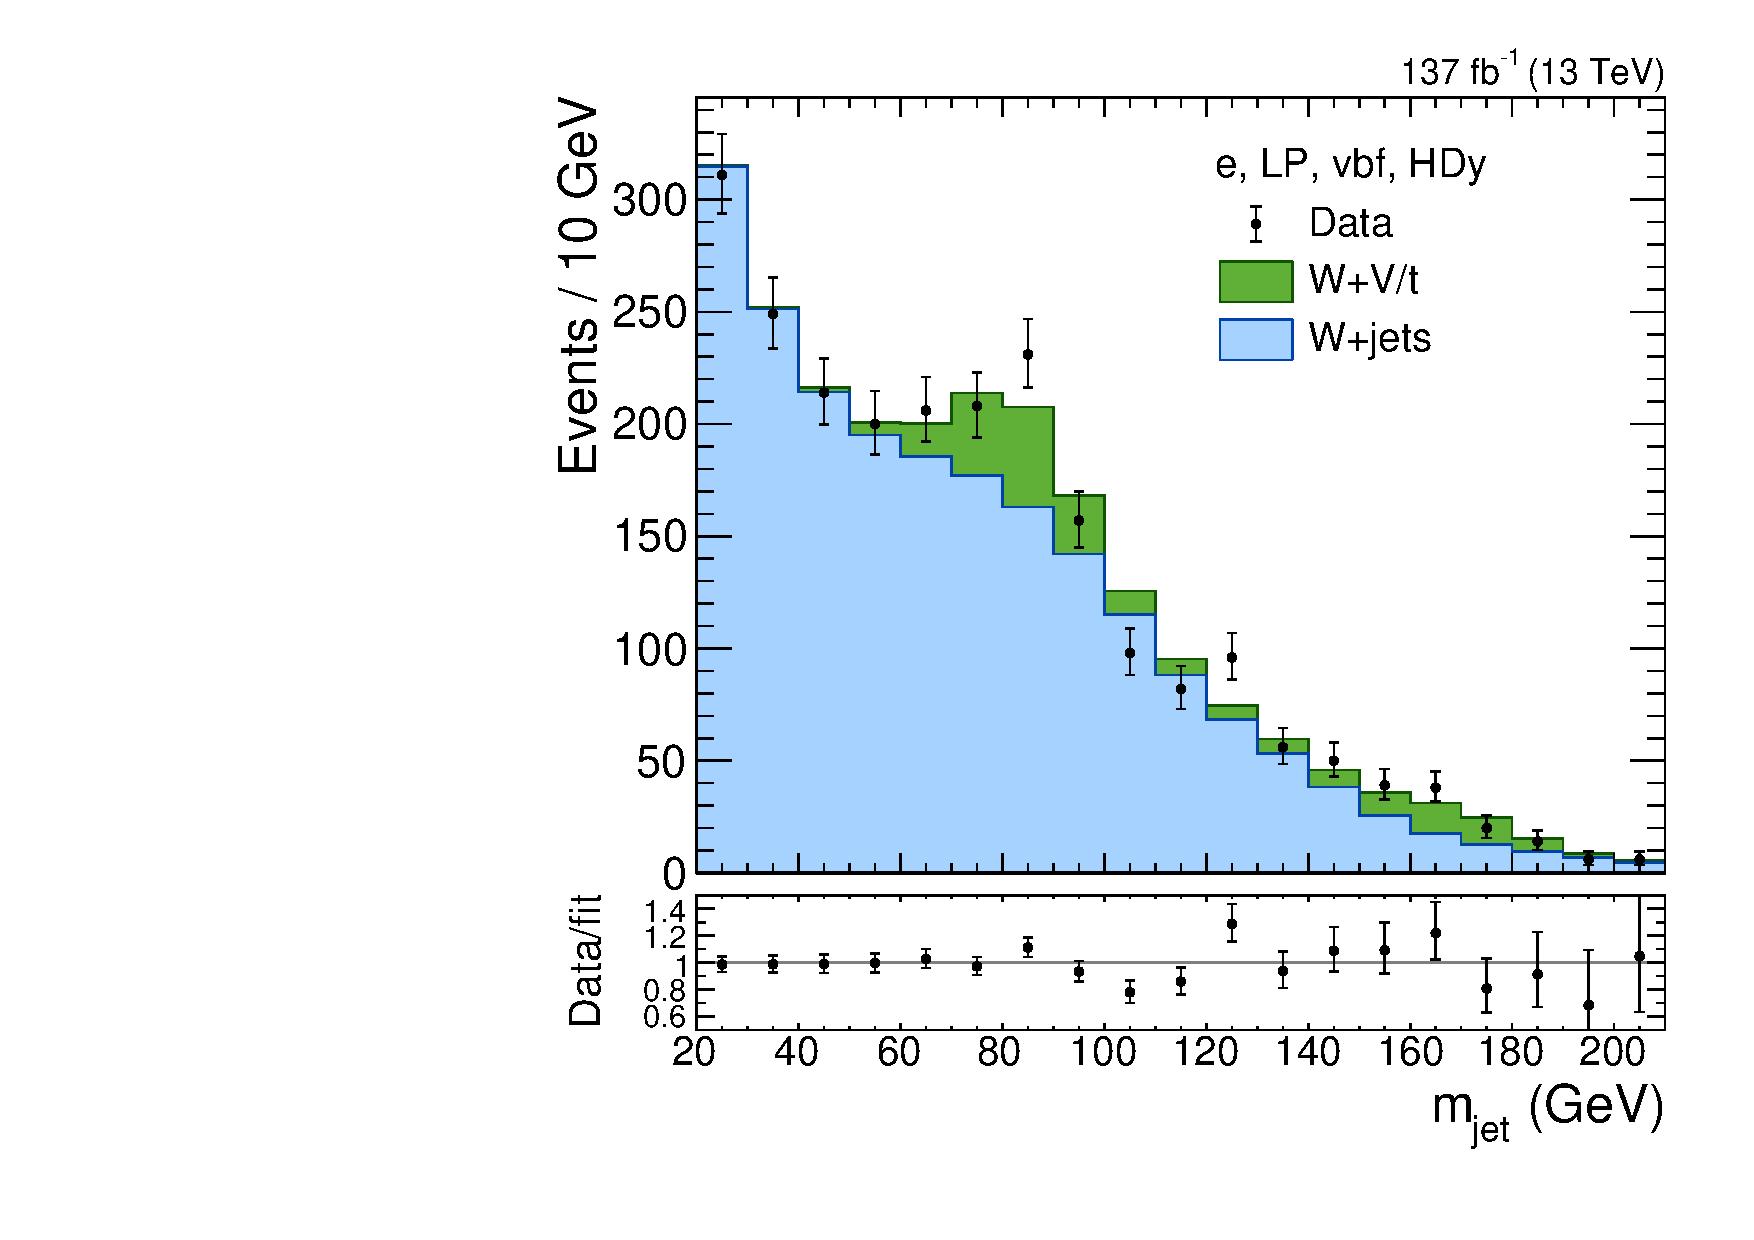
\includegraphics[width=0.18\textwidth]{fig/fitValidation/PostFit_SR_MJJ__e_LP_vbf_HDy_Run2.pdf}\\
  \caption{
    Post-fit distributions and data projected onto the \MJ dimension for the full range of \MVV.
    Columns 1 to 4: $\mu$-HP, $e$-HP, $\mu$-LP, and $e$-LP.
    Rows 1 to 6: bb-LDy, nobb-LDy, vbf-LDy, bb-HDy, nobb-HDy, and vbf-HDy.
  }
  \label{fig:postfit_MJJ_Run2}
\end{figure}

\begin{figure}[htbp]
  \centering
  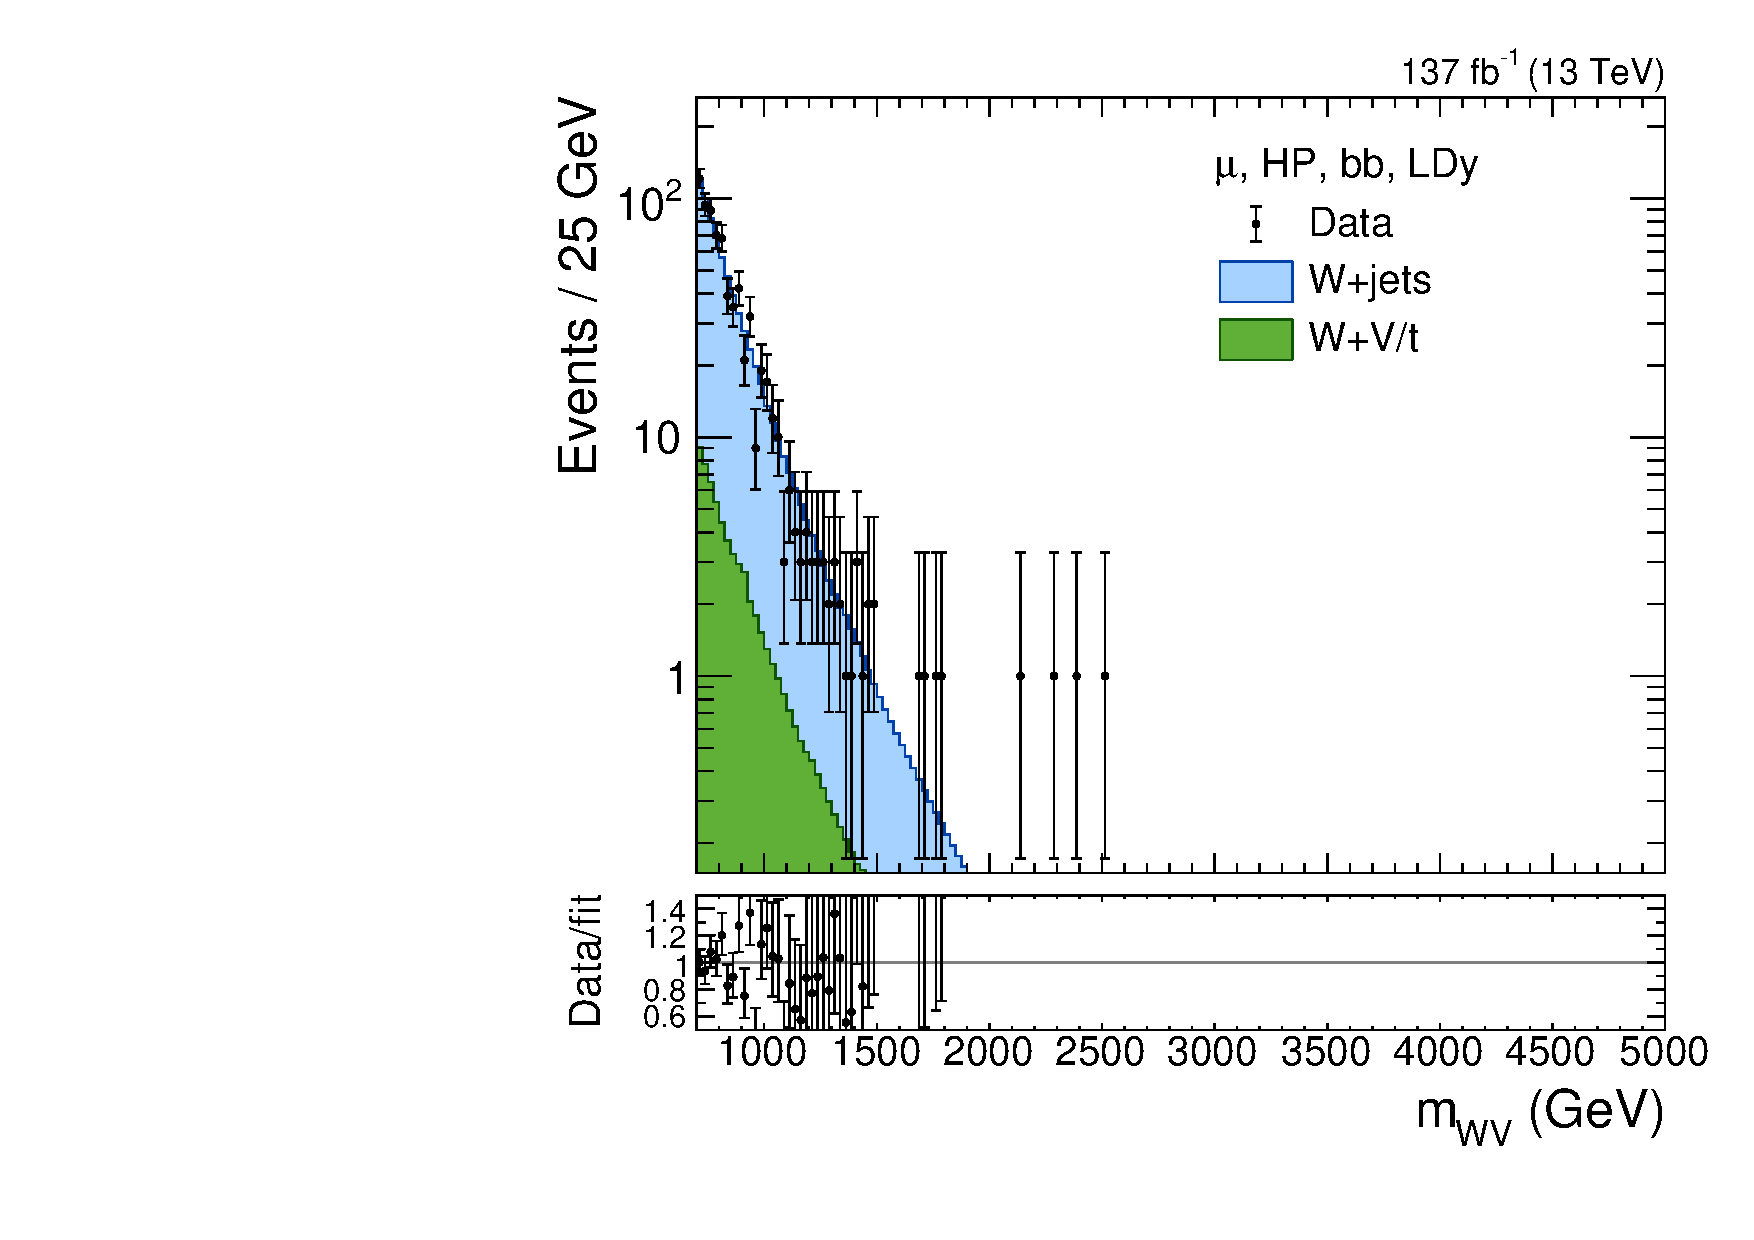
\includegraphics[width=0.18\textwidth]{fig/fitValidation/PostFit_SR_MVV__mu_HP_bb_LDy_Run2.pdf}
  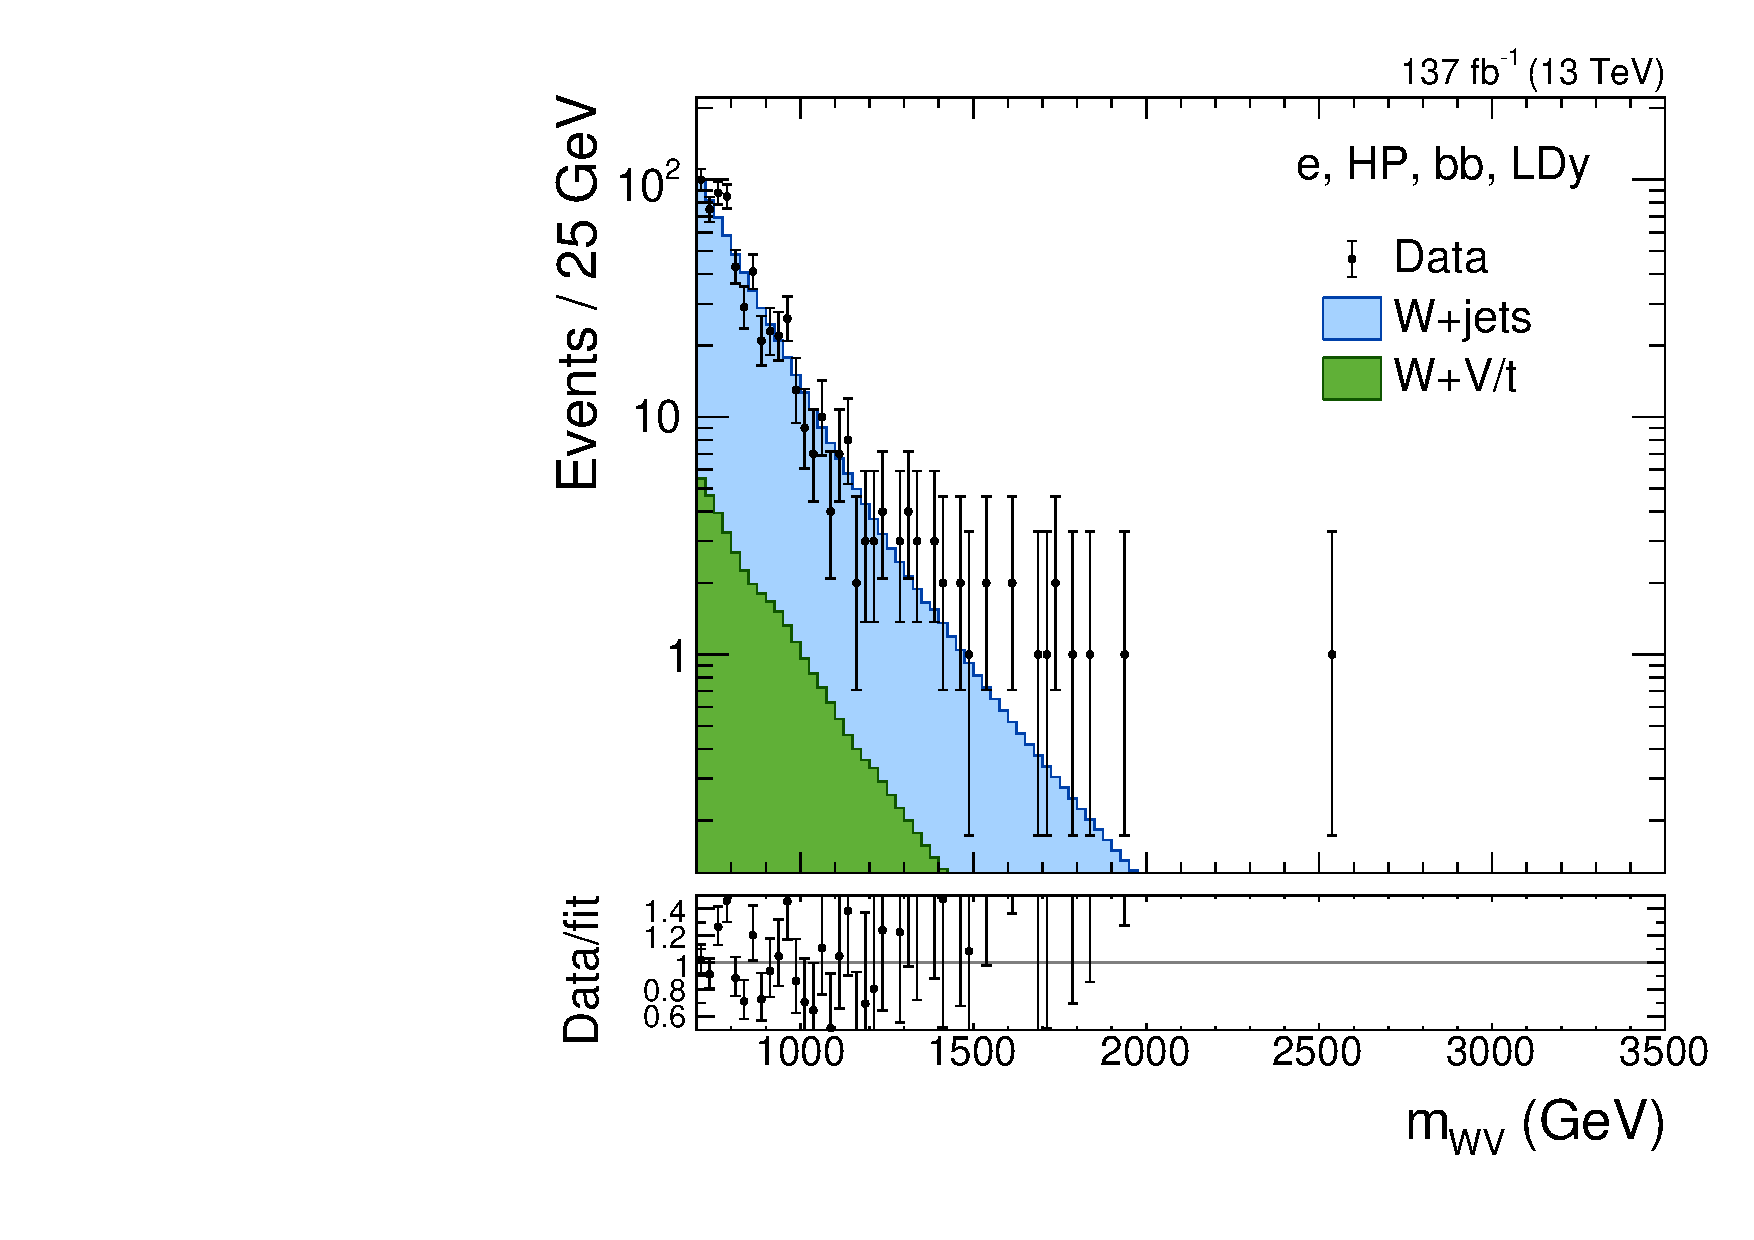
\includegraphics[width=0.18\textwidth]{fig/fitValidation/PostFit_SR_MVV__e_HP_bb_LDy_Run2.pdf}
  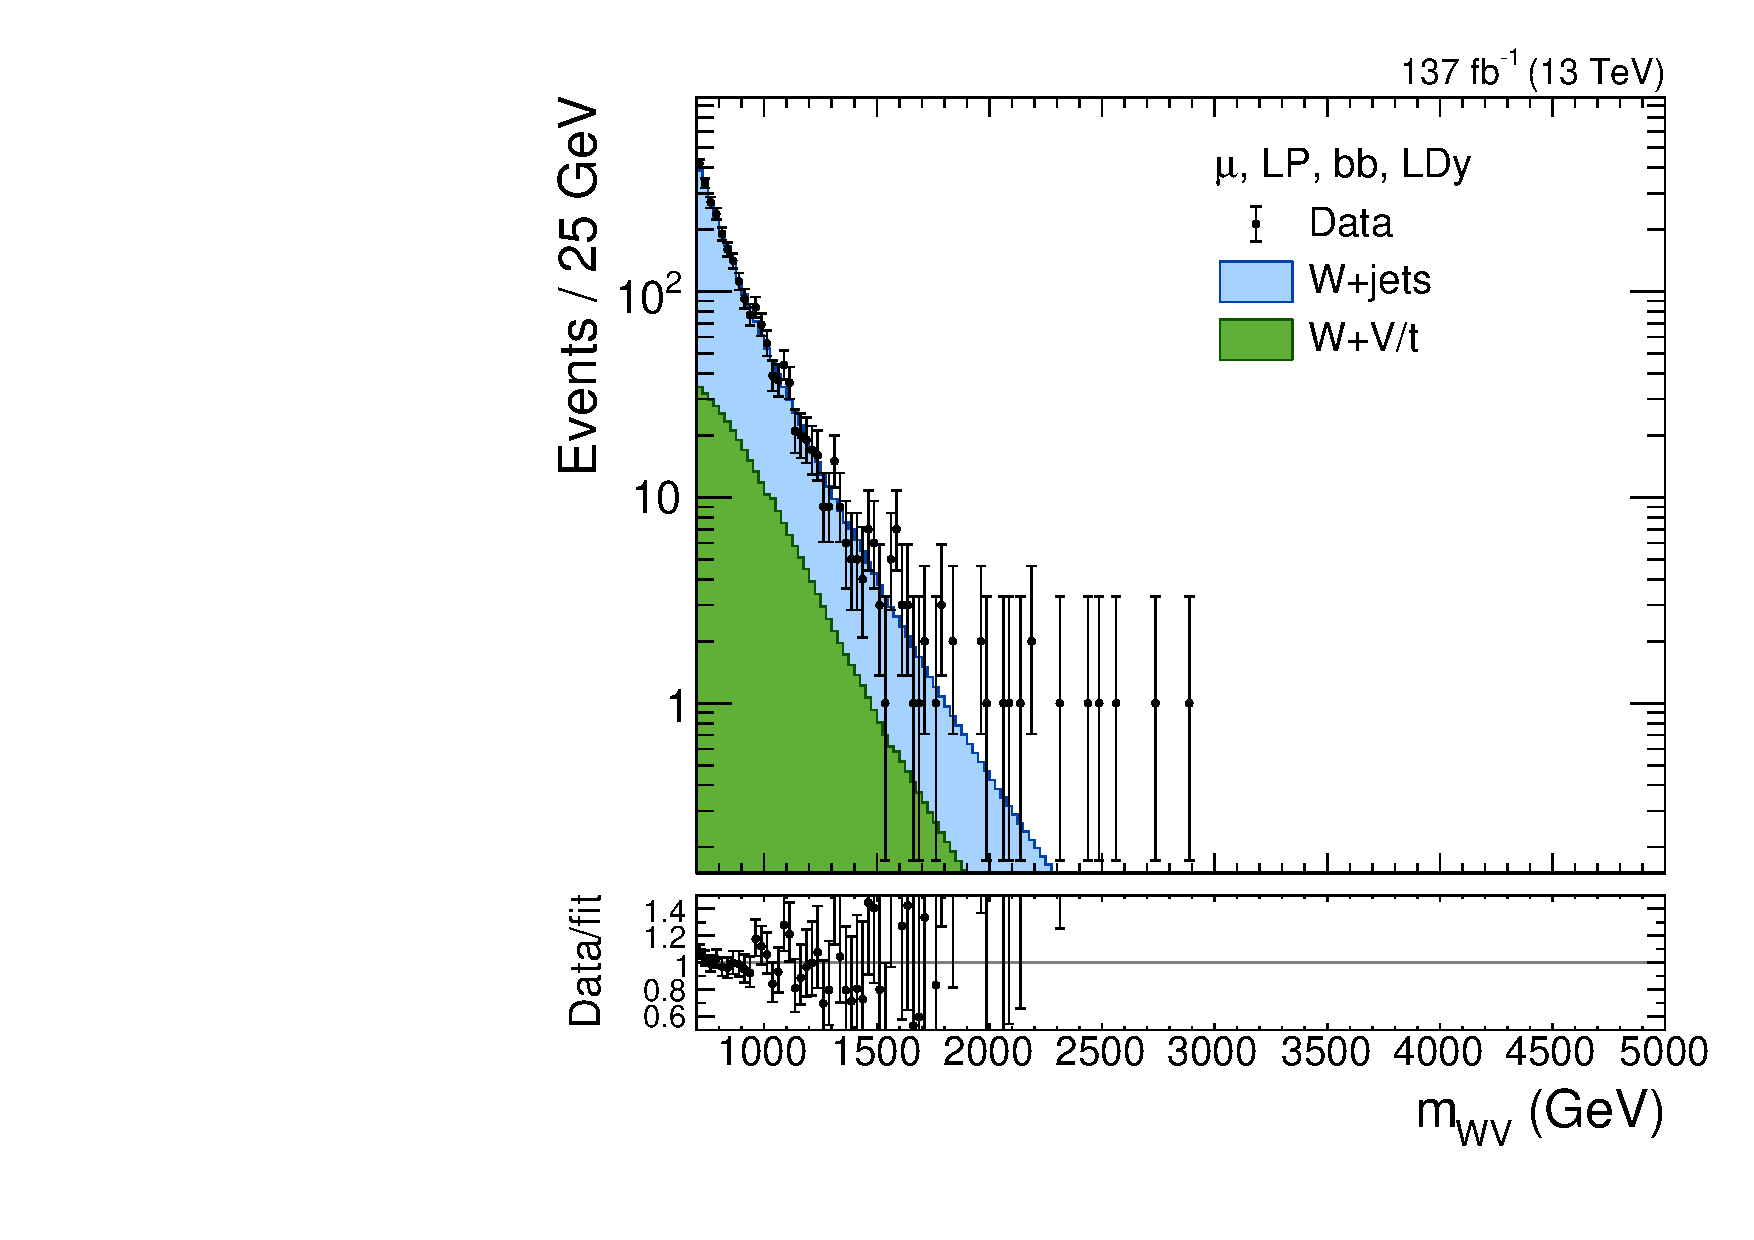
\includegraphics[width=0.18\textwidth]{fig/fitValidation/PostFit_SR_MVV__mu_LP_bb_LDy_Run2.pdf}
  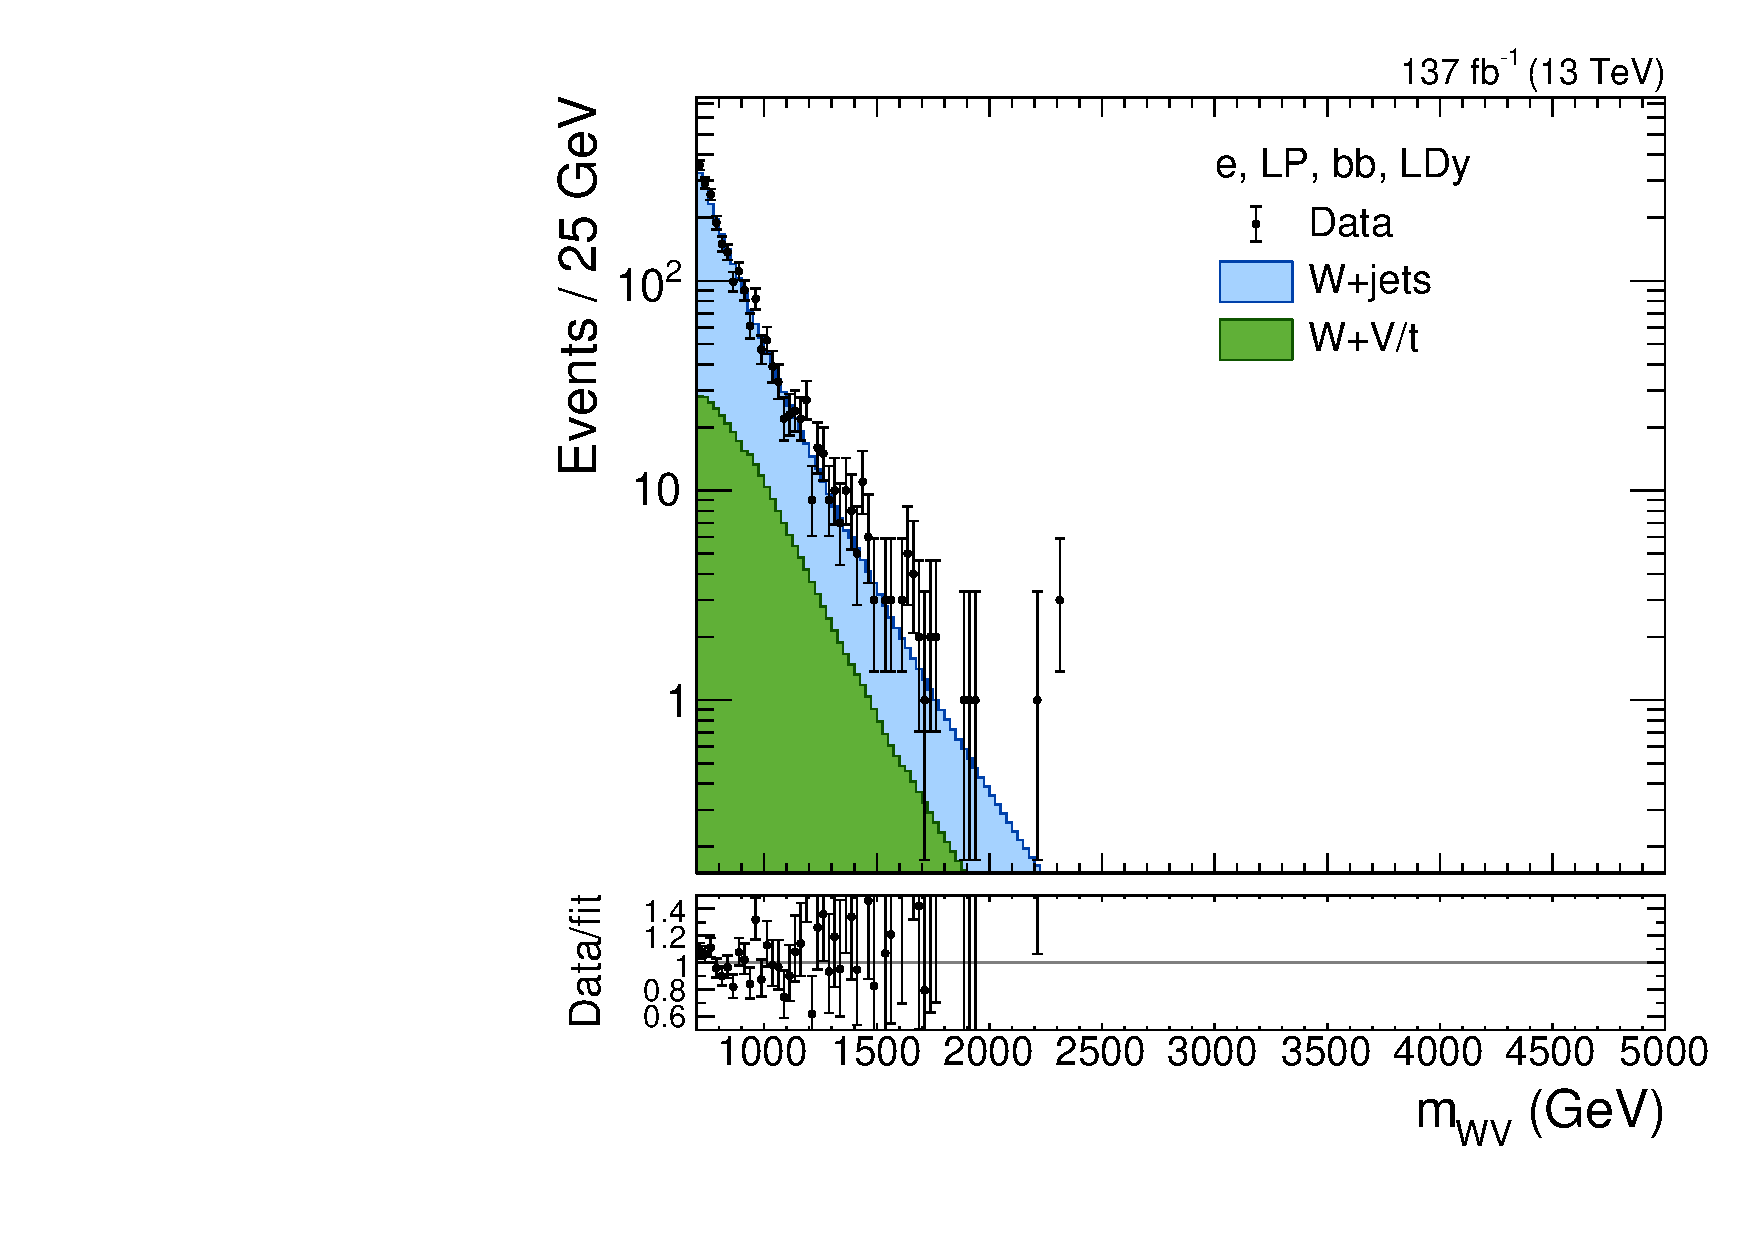
\includegraphics[width=0.18\textwidth]{fig/fitValidation/PostFit_SR_MVV__e_LP_bb_LDy_Run2.pdf}\\
  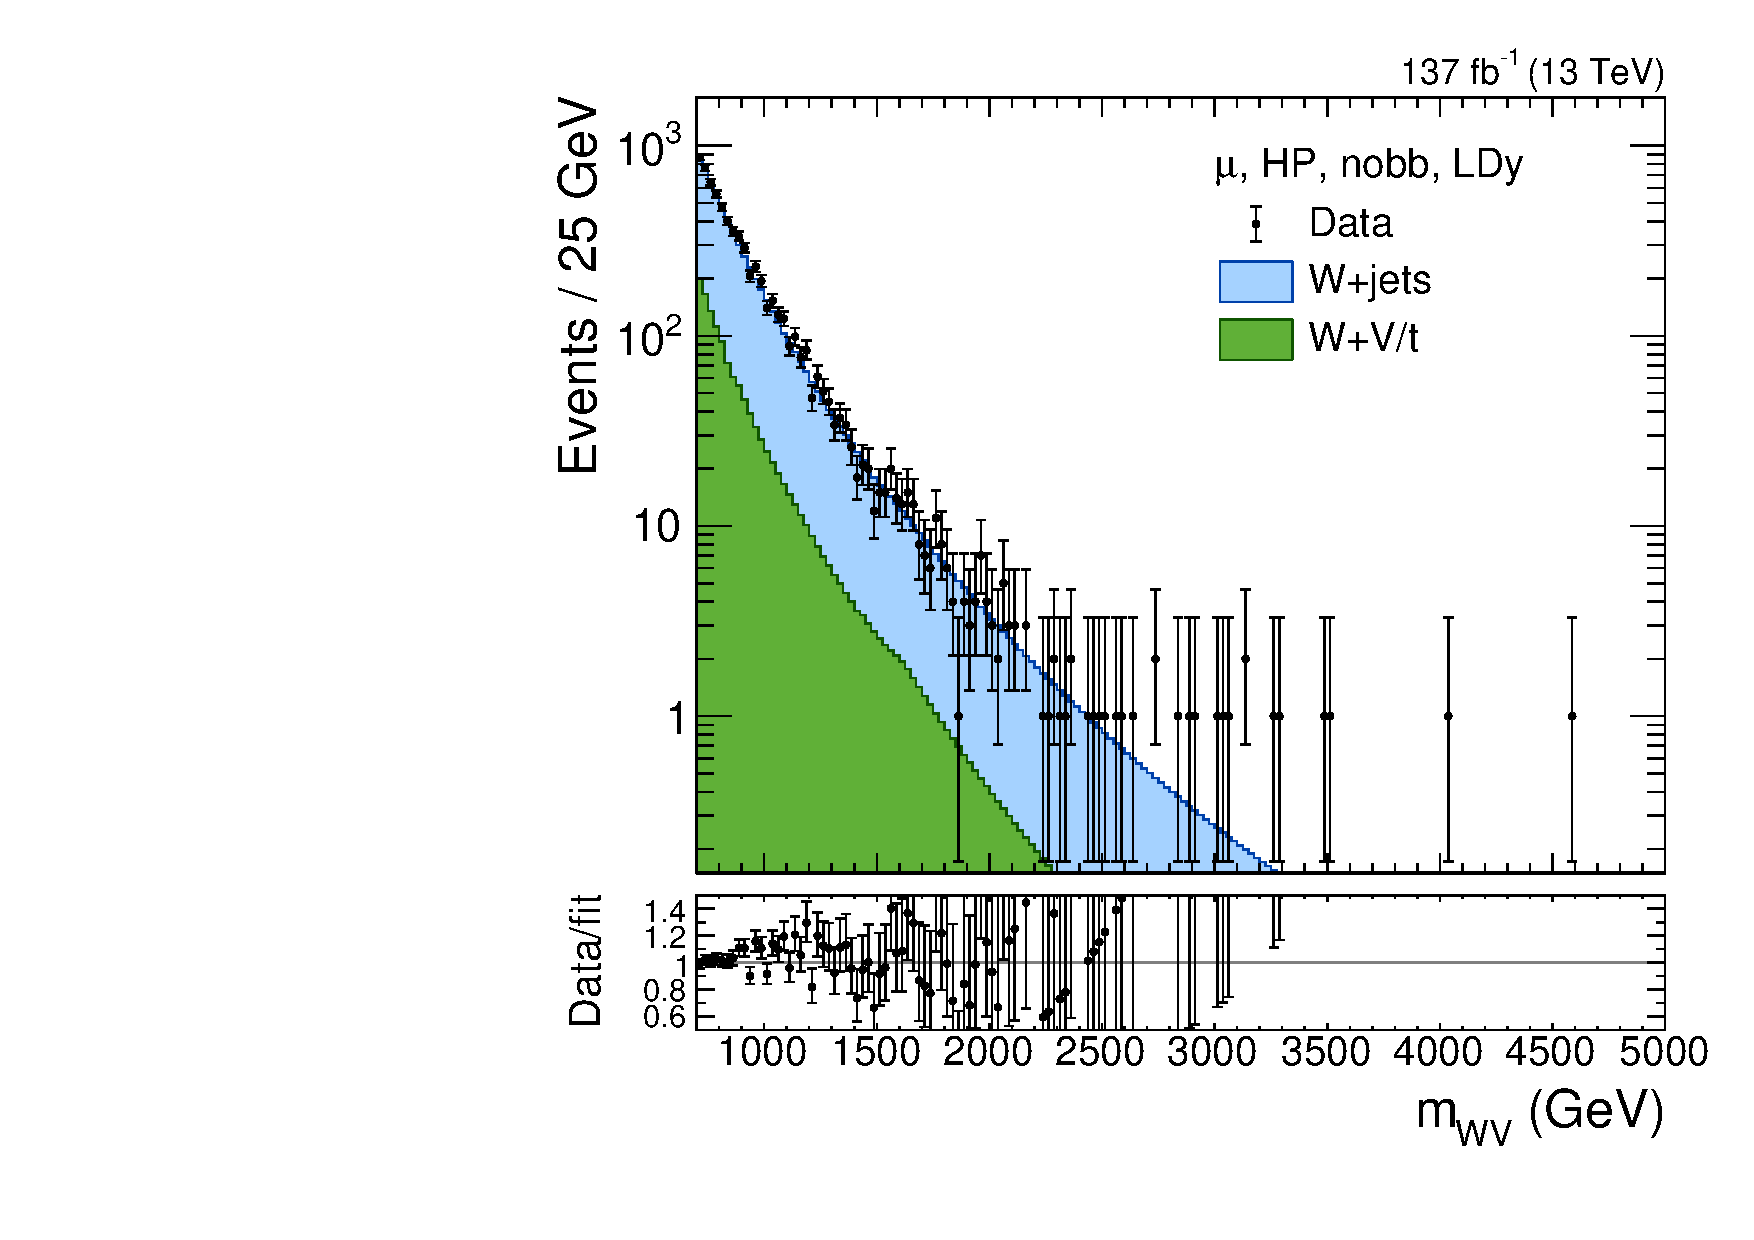
\includegraphics[width=0.18\textwidth]{fig/fitValidation/PostFit_SR_MVV__mu_HP_nobb_LDy_Run2.pdf}
  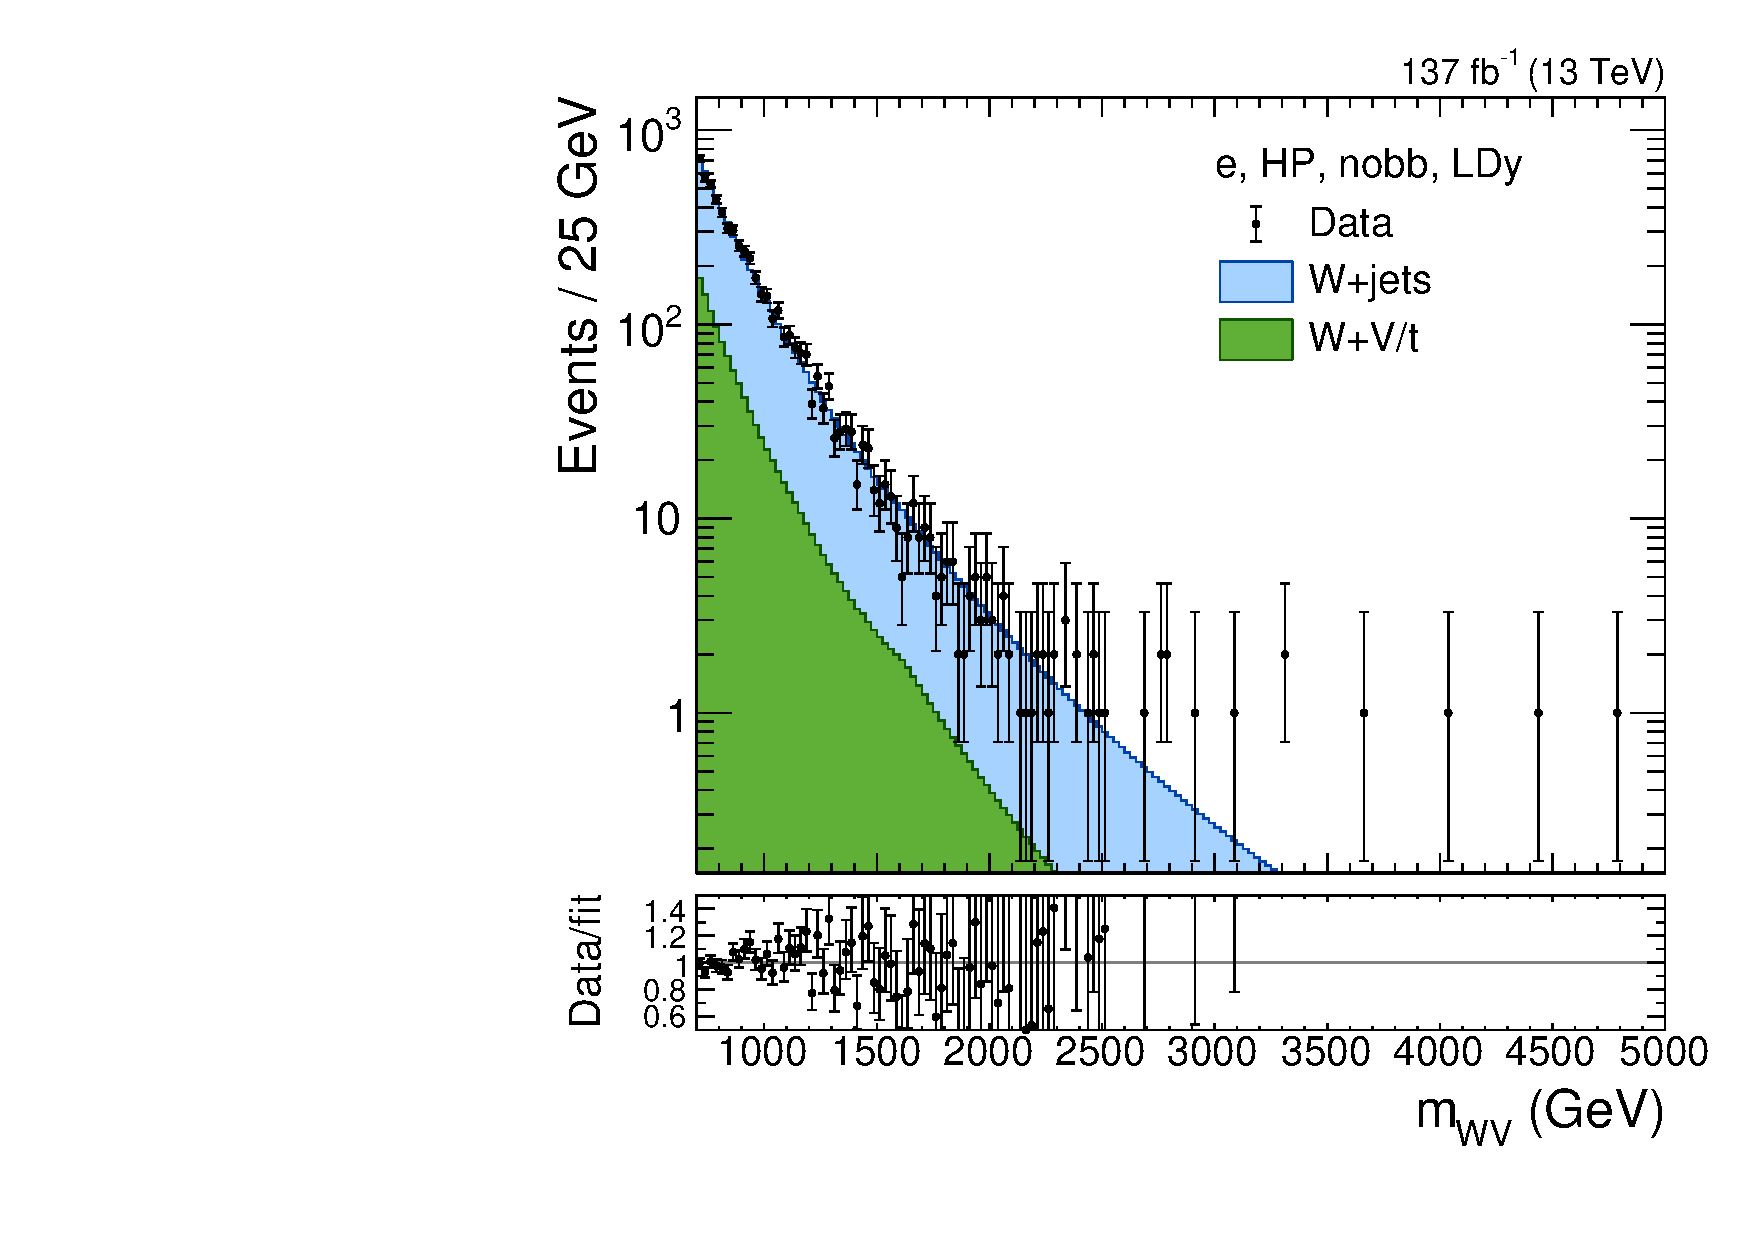
\includegraphics[width=0.18\textwidth]{fig/fitValidation/PostFit_SR_MVV__e_HP_nobb_LDy_Run2.pdf}
  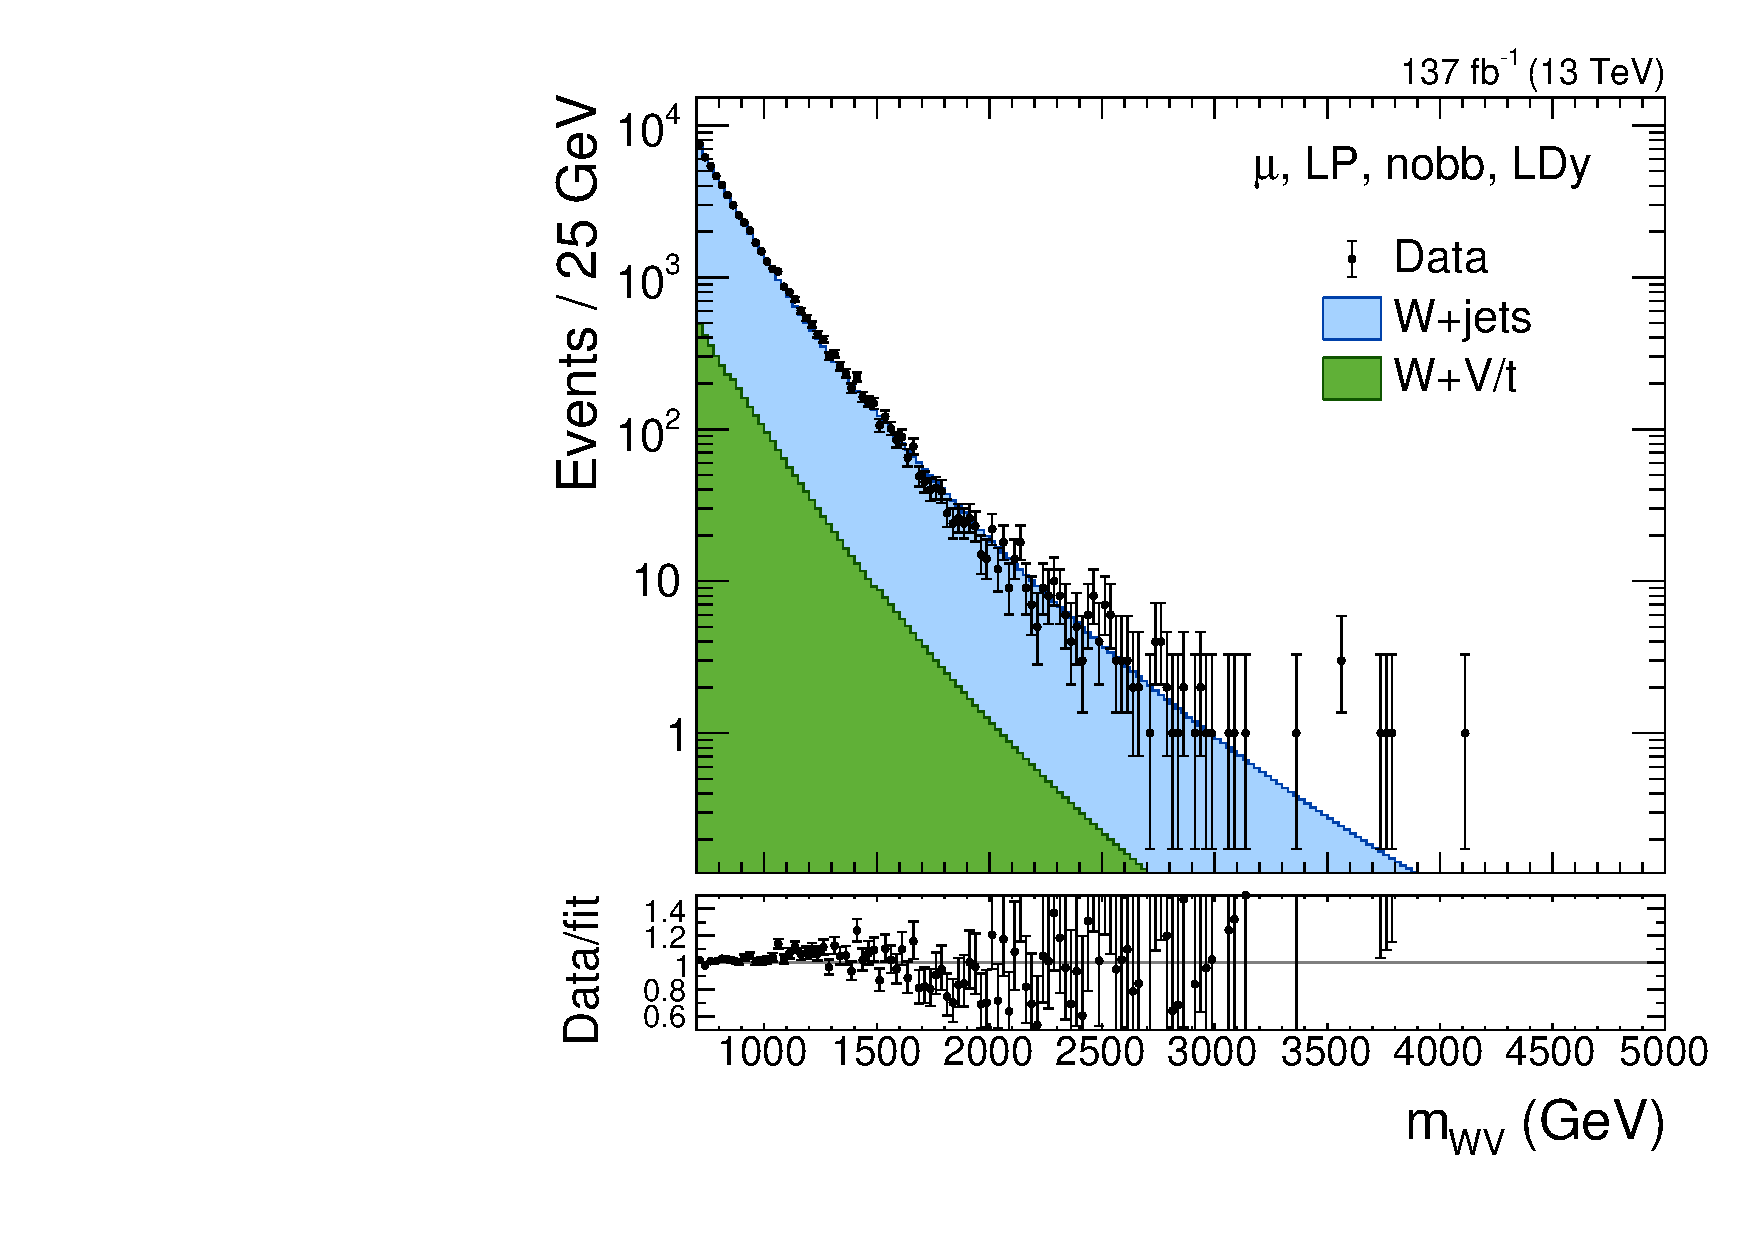
\includegraphics[width=0.18\textwidth]{fig/fitValidation/PostFit_SR_MVV__mu_LP_nobb_LDy_Run2.pdf}
  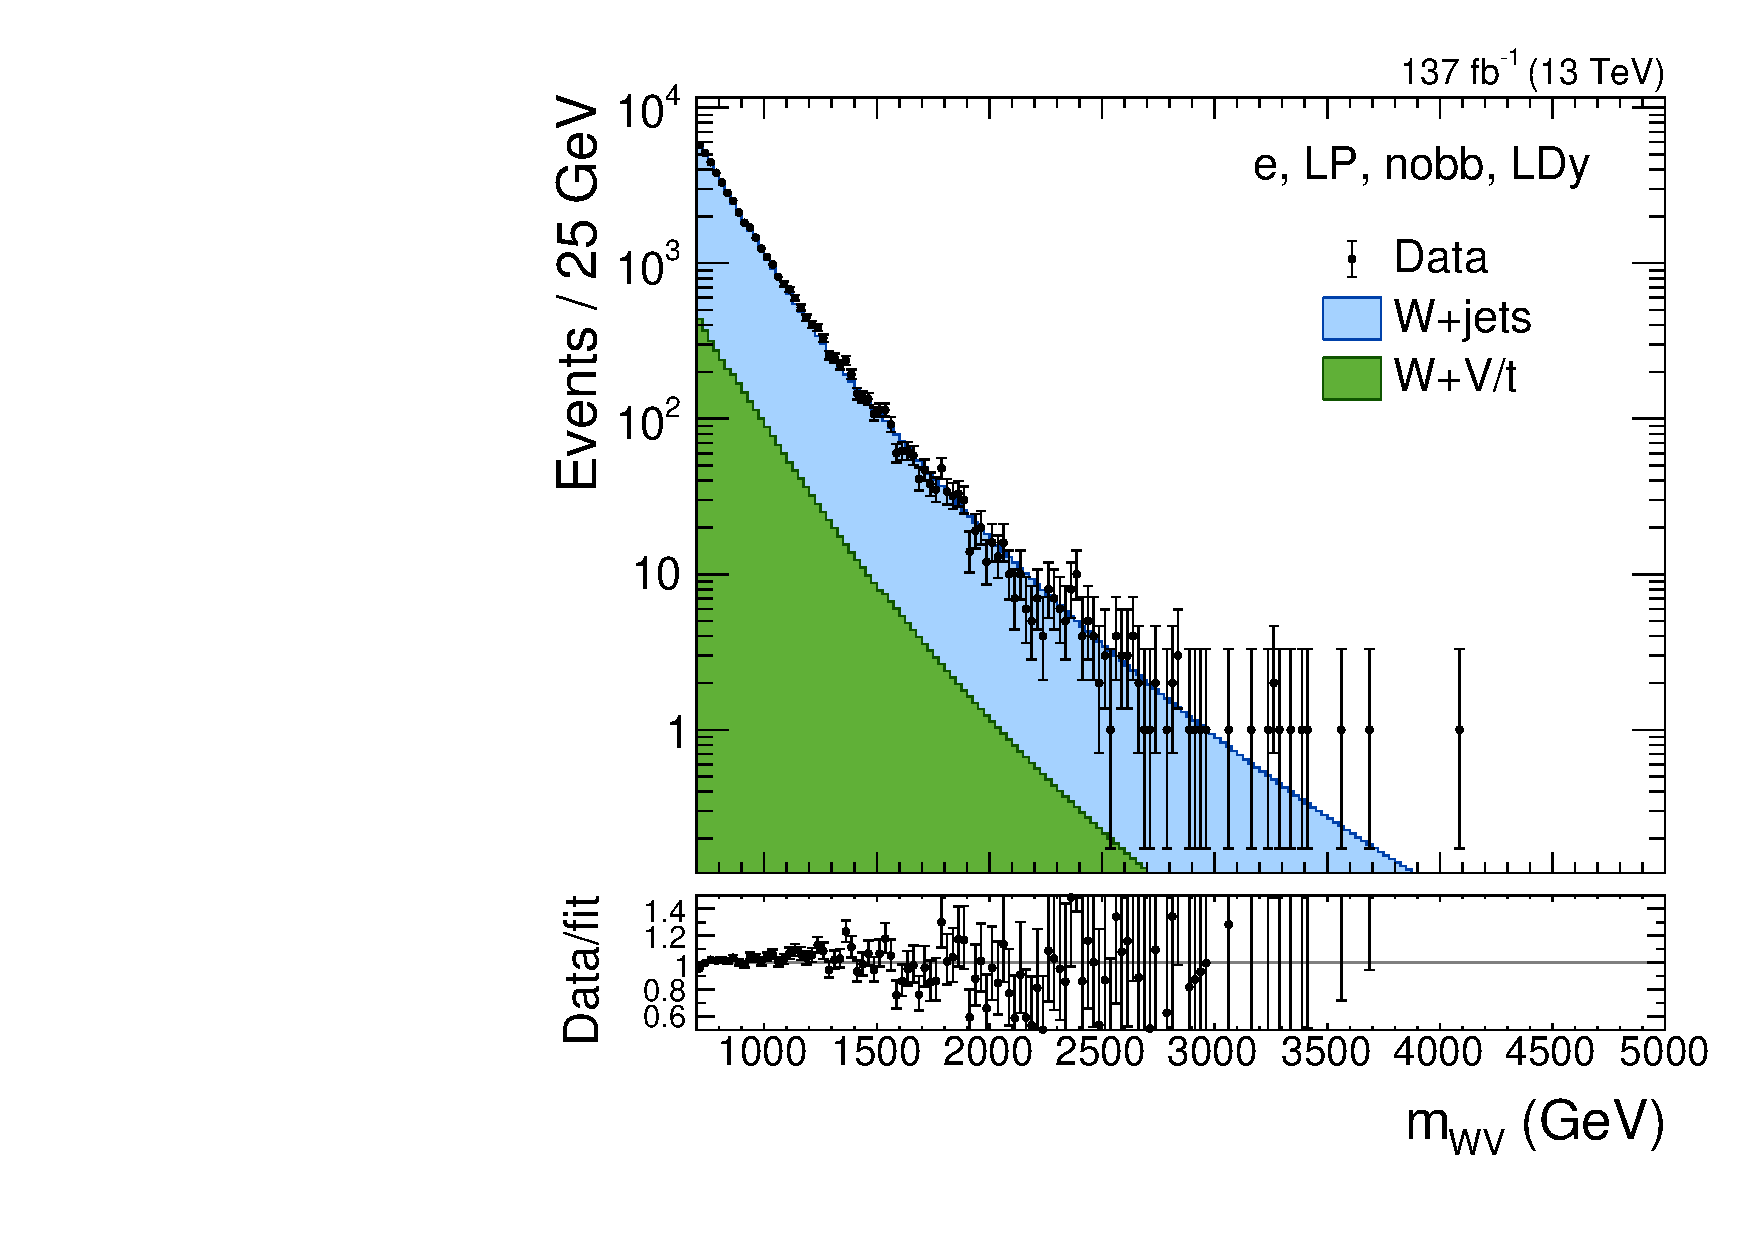
\includegraphics[width=0.18\textwidth]{fig/fitValidation/PostFit_SR_MVV__e_LP_nobb_LDy_Run2.pdf}\\
  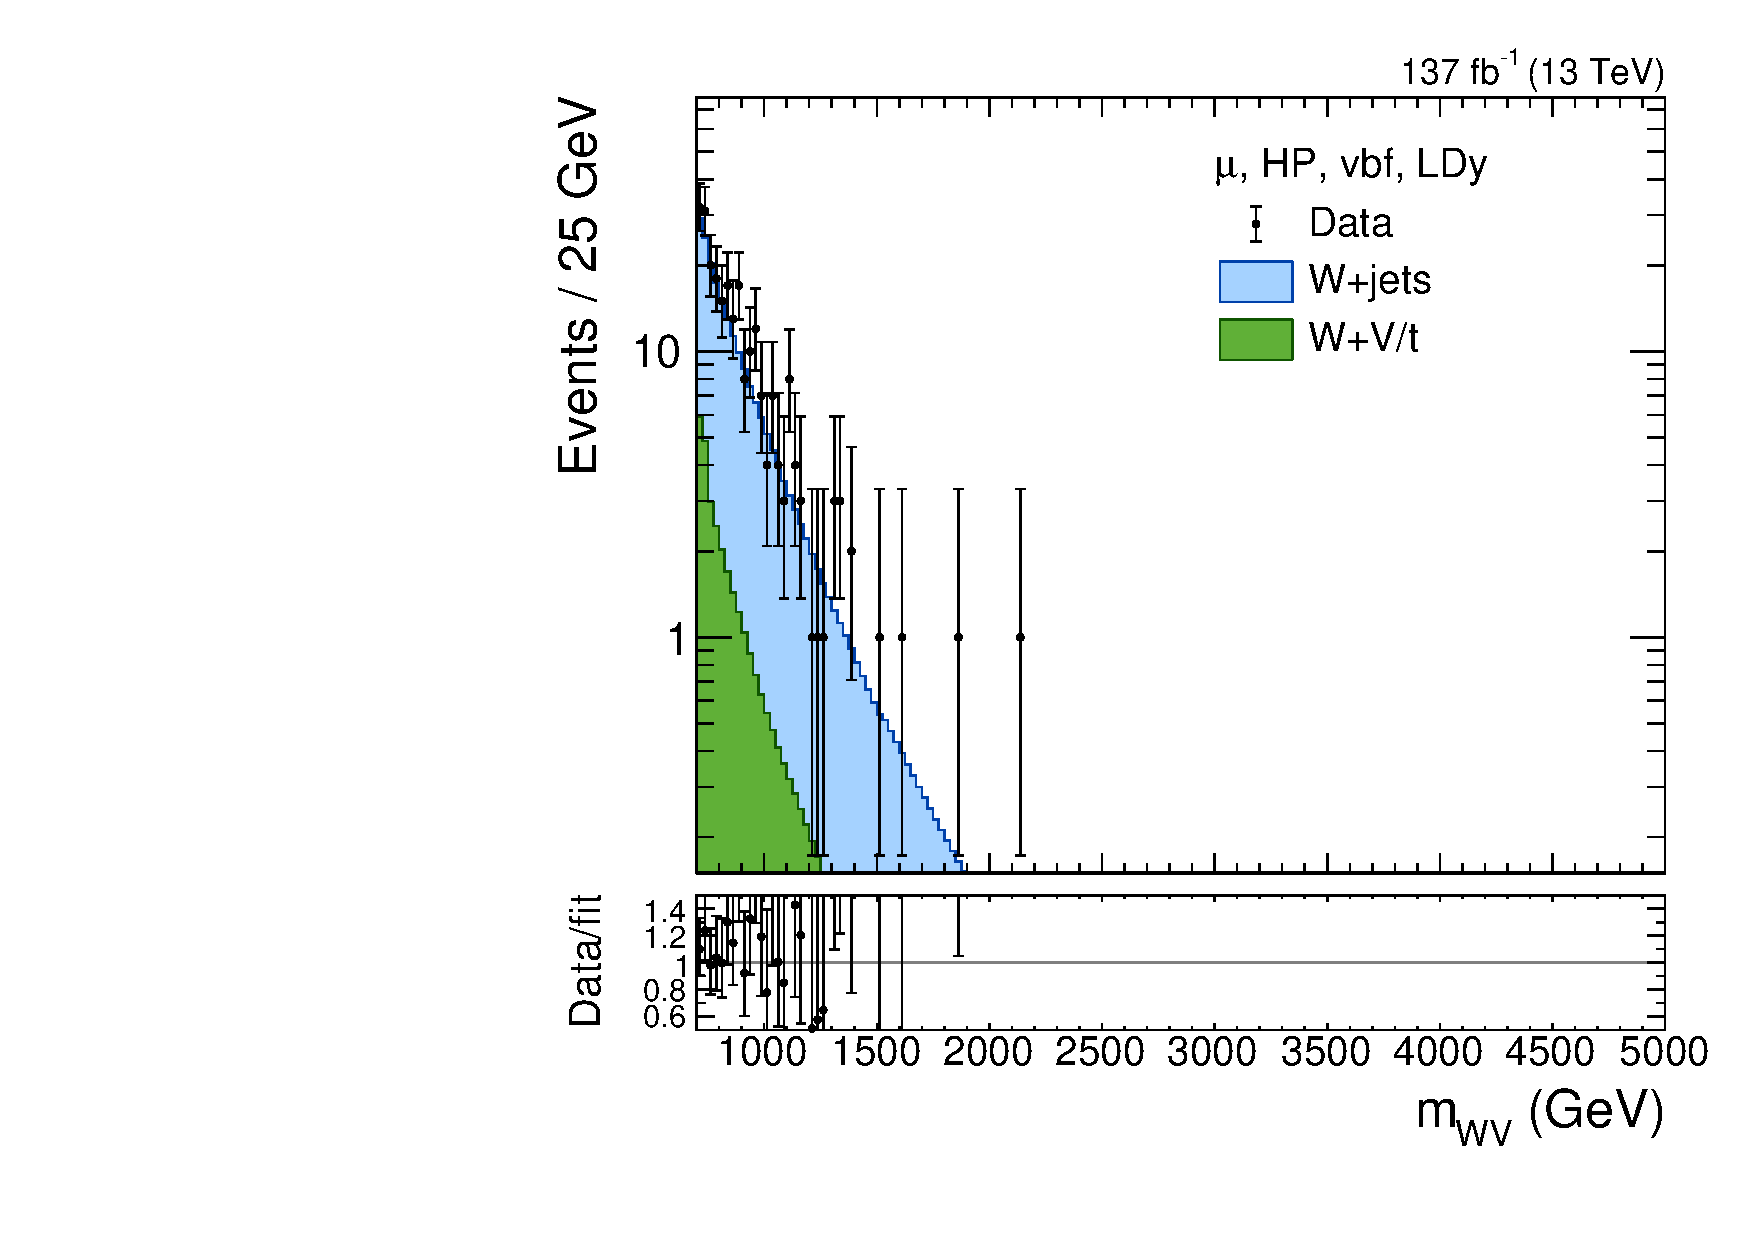
\includegraphics[width=0.18\textwidth]{fig/fitValidation/PostFit_SR_MVV__mu_HP_vbf_LDy_Run2.pdf}
  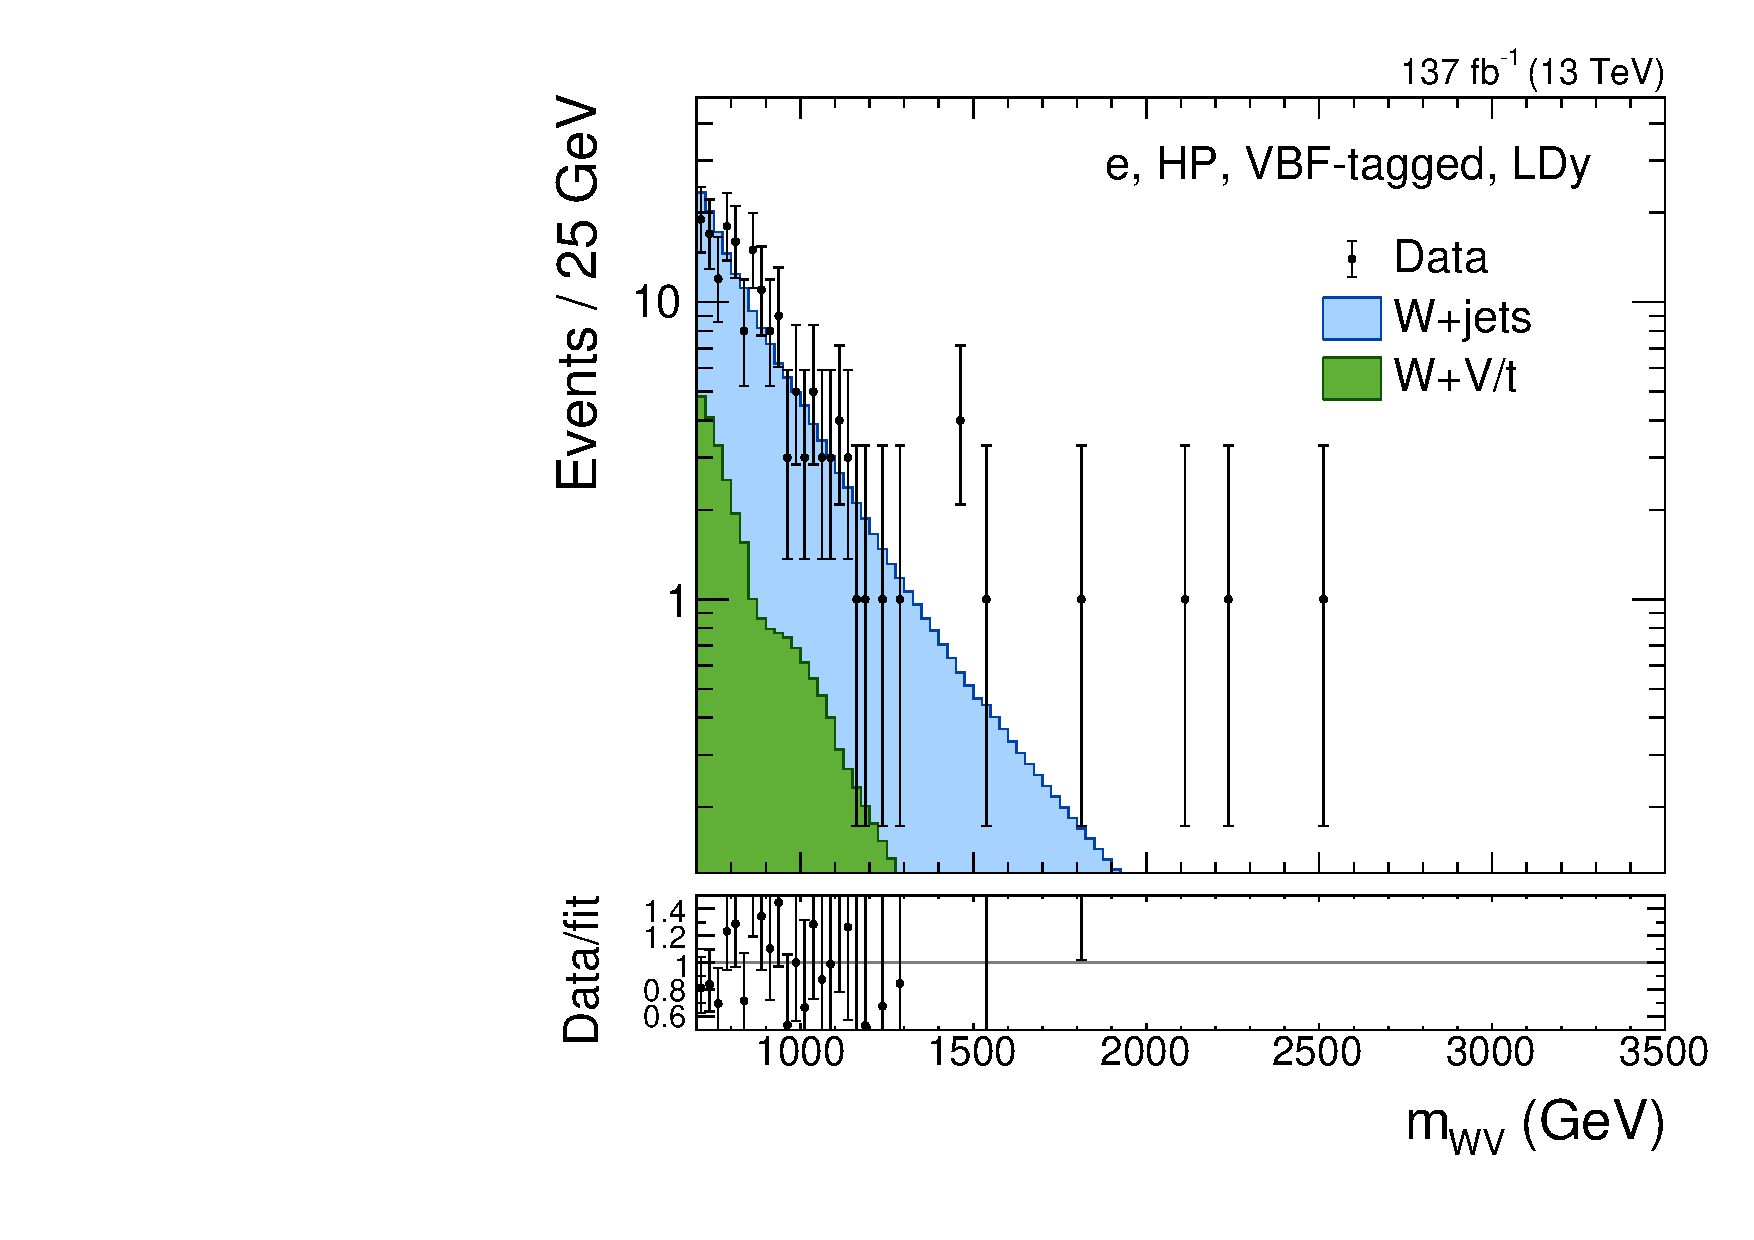
\includegraphics[width=0.18\textwidth]{fig/fitValidation/PostFit_SR_MVV__e_HP_vbf_LDy_Run2.pdf}
  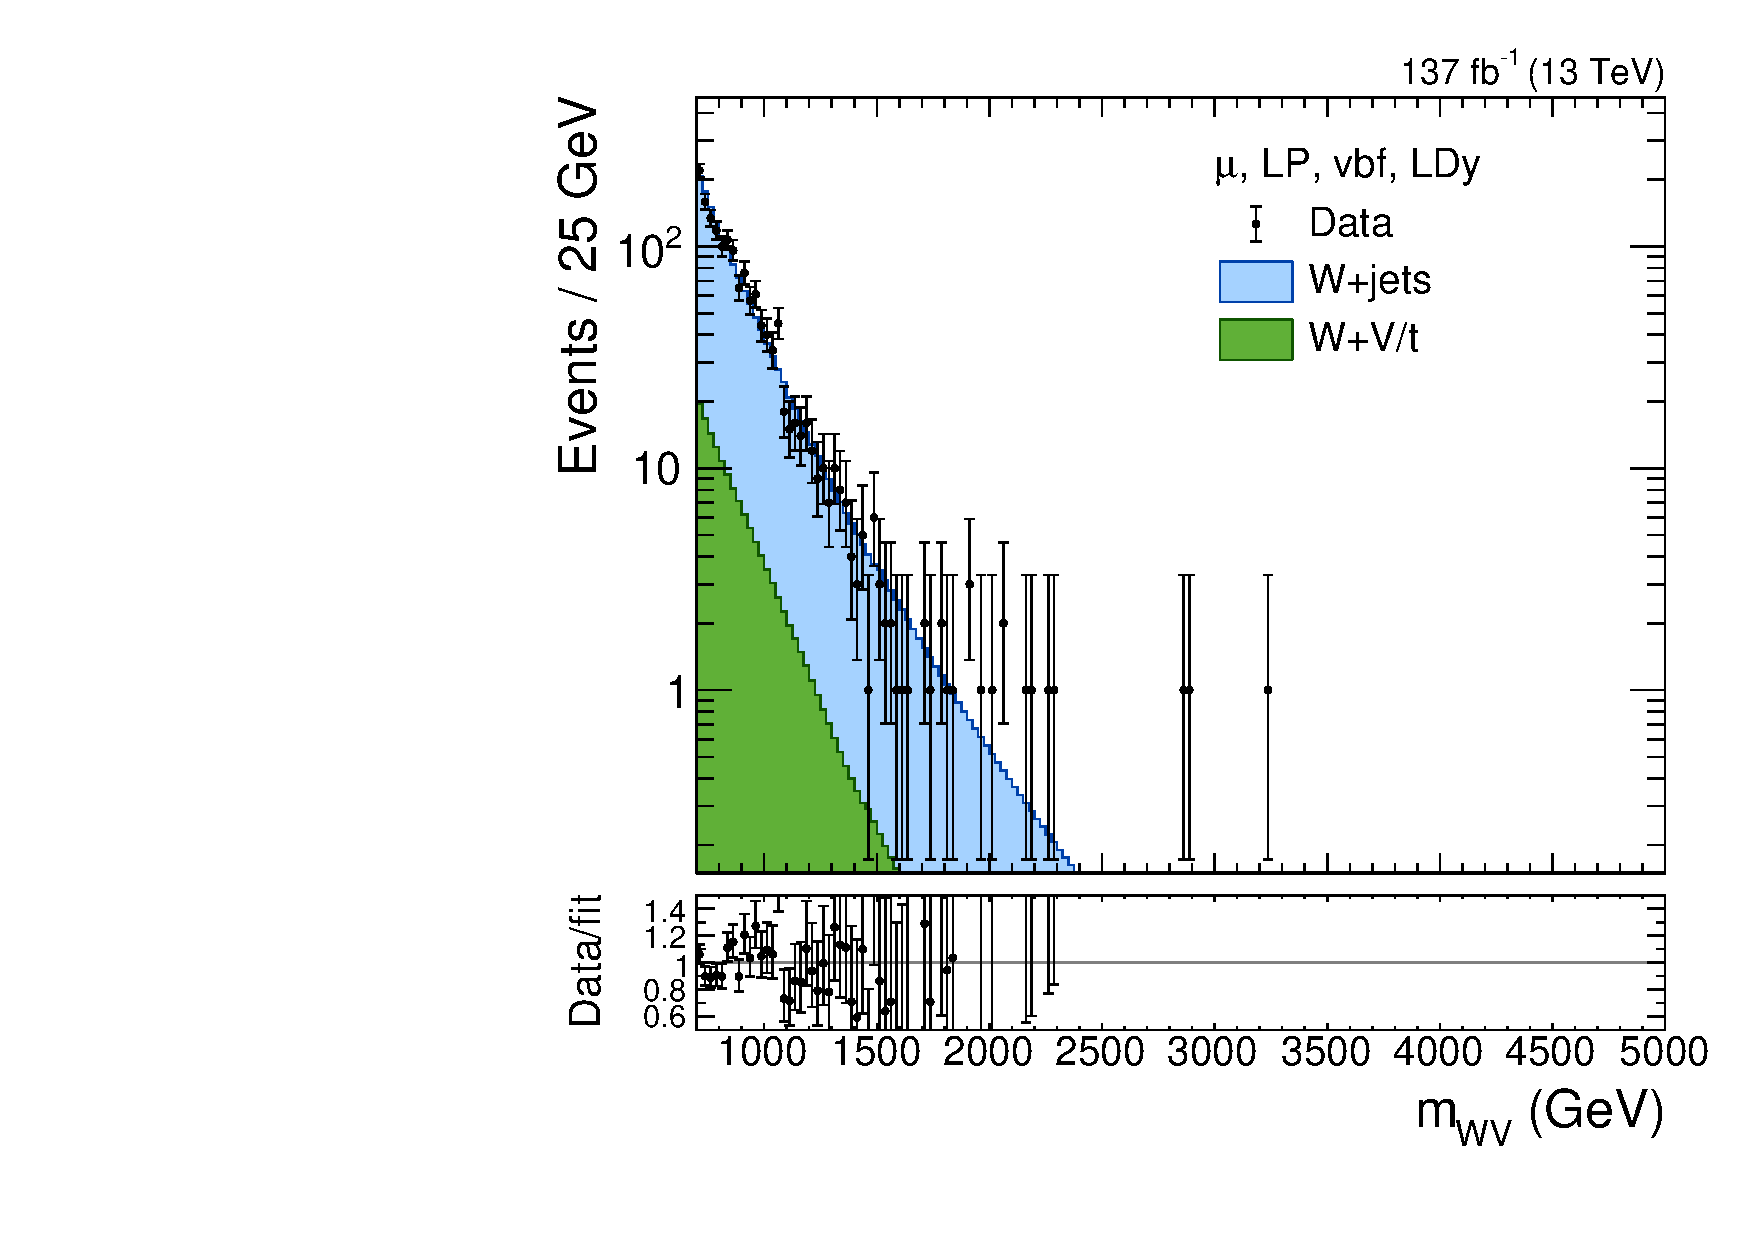
\includegraphics[width=0.18\textwidth]{fig/fitValidation/PostFit_SR_MVV__mu_LP_vbf_LDy_Run2.pdf}
  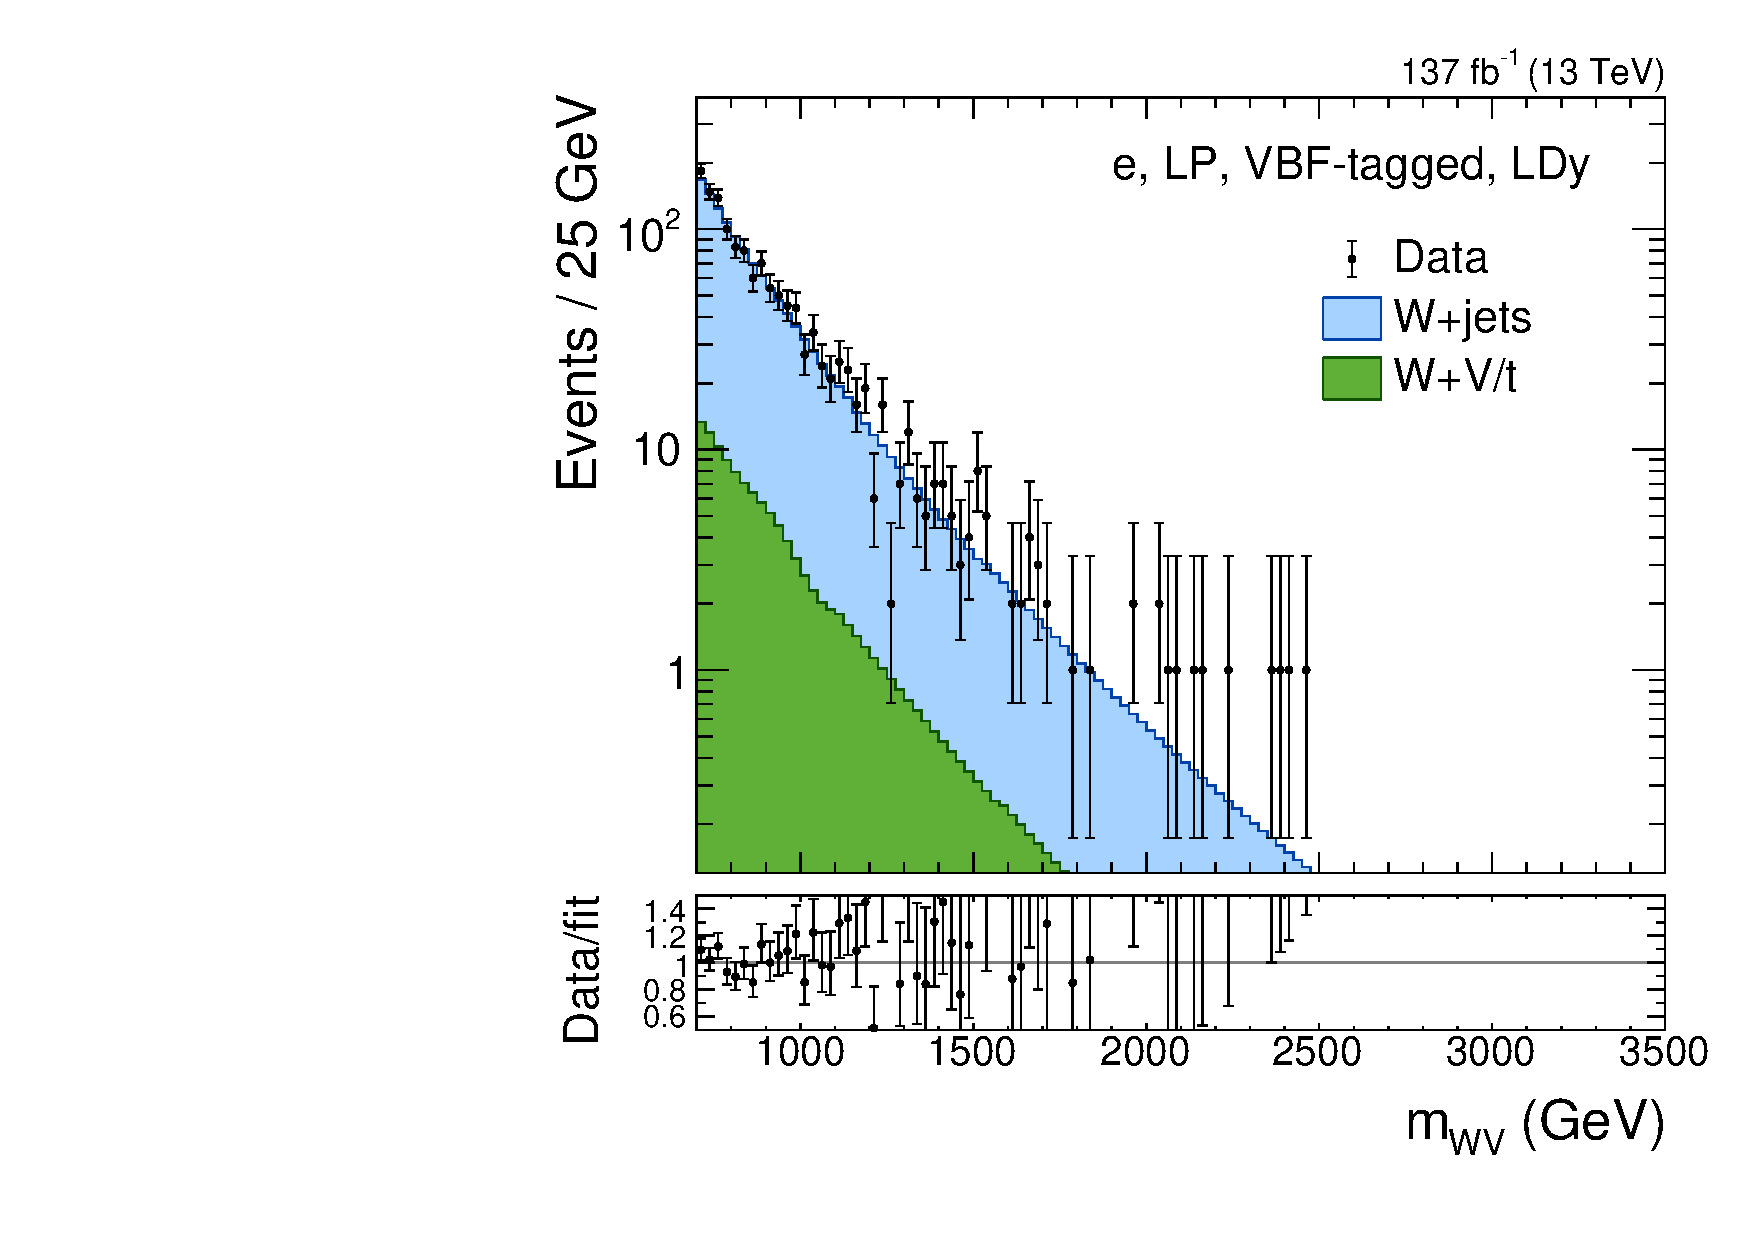
\includegraphics[width=0.18\textwidth]{fig/fitValidation/PostFit_SR_MVV__e_LP_vbf_LDy_Run2.pdf}\\
  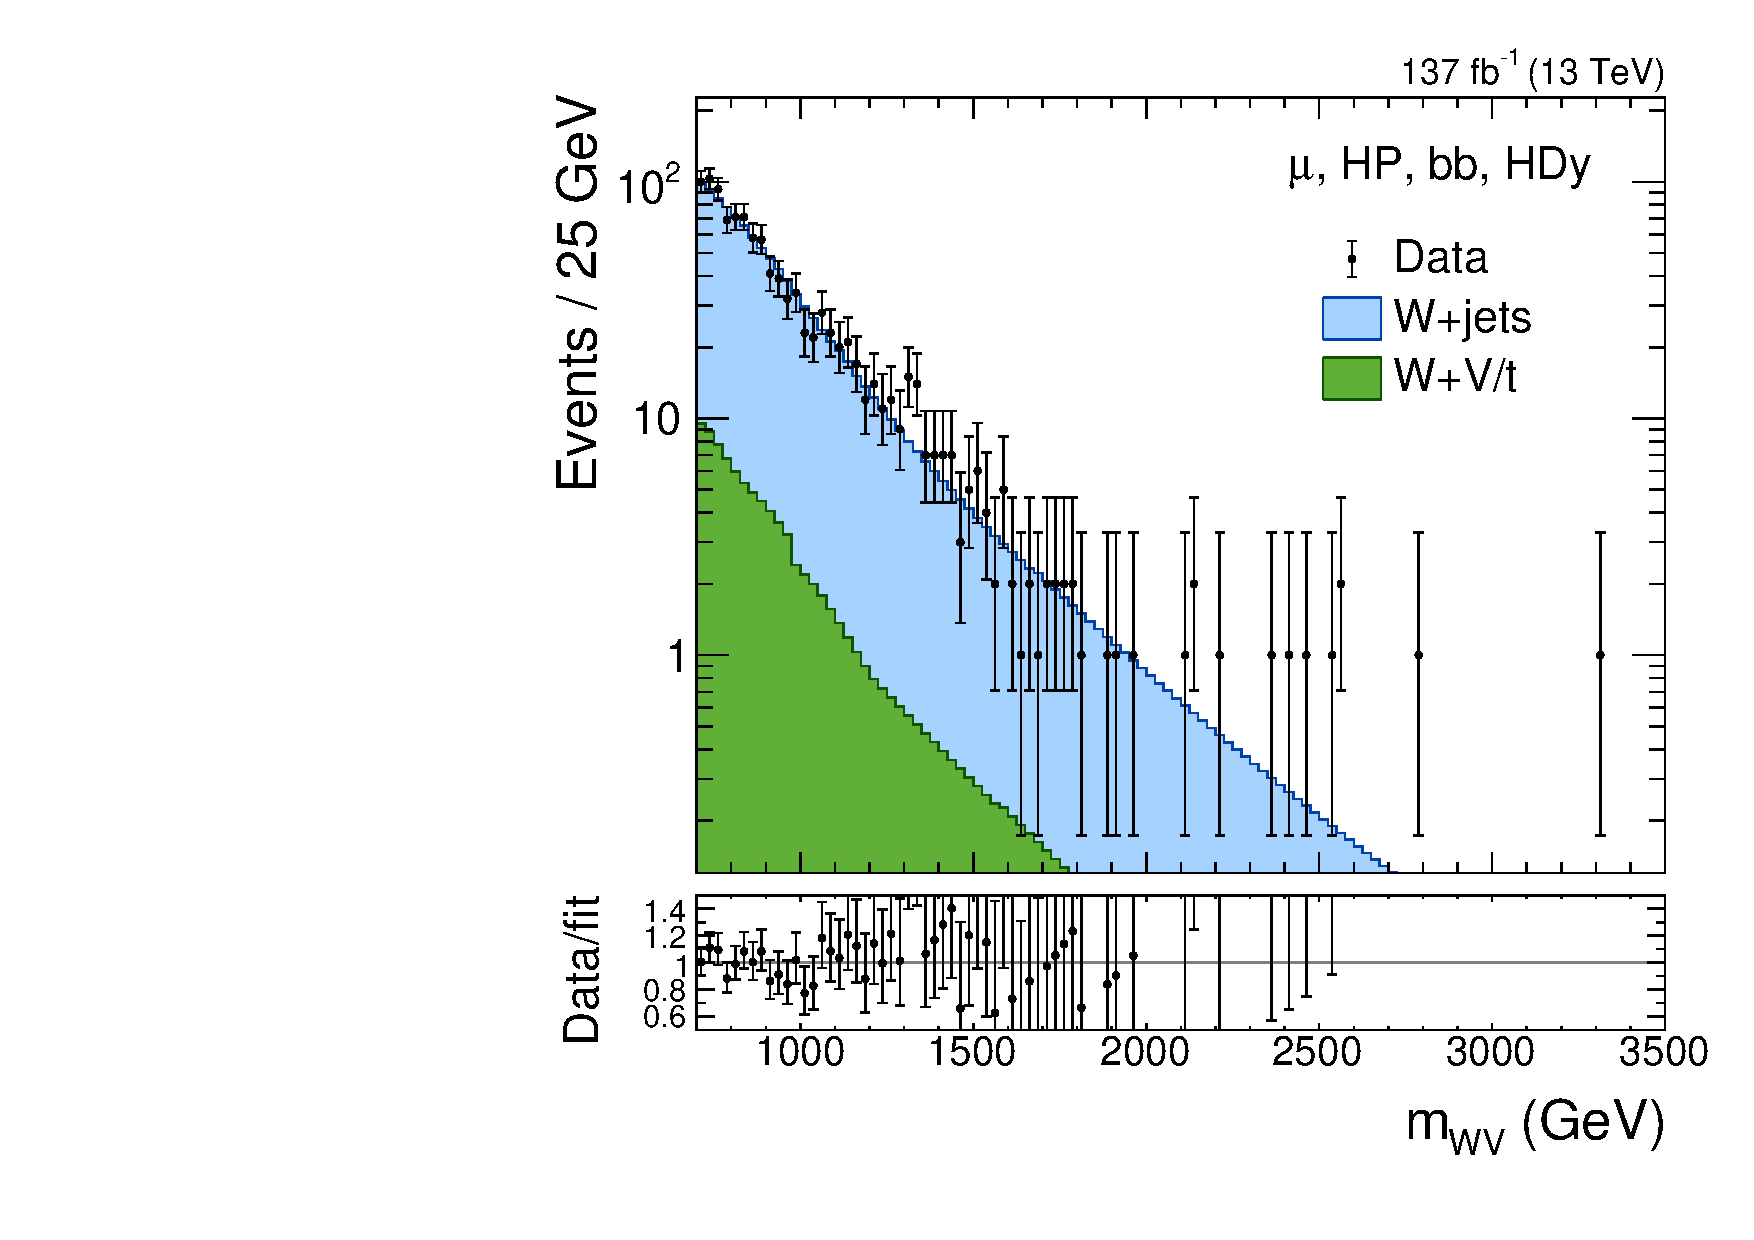
\includegraphics[width=0.18\textwidth]{fig/fitValidation/PostFit_SR_MVV__mu_HP_bb_HDy_Run2.pdf}
  \includegraphics[width=0.18\textwidth]{fig/fitValidation/PostFit_SR_MVV__e_HP_bb_HDy_Run2.pdf}
  \includegraphics[width=0.18\textwidth]{fig/fitValidation/PostFit_SR_MVV__mu_LP_bb_HDy_Run2.pdf}
  \includegraphics[width=0.18\textwidth]{fig/fitValidation/PostFit_SR_MVV__e_LP_bb_HDy_Run2.pdf}\\
  \includegraphics[width=0.18\textwidth]{fig/fitValidation/PostFit_SR_MVV__mu_HP_nobb_HDy_Run2.pdf}
  \includegraphics[width=0.18\textwidth]{fig/fitValidation/PostFit_SR_MVV__e_HP_nobb_HDy_Run2.pdf}
  \includegraphics[width=0.18\textwidth]{fig/fitValidation/PostFit_SR_MVV__mu_LP_nobb_HDy_Run2.pdf}
  \includegraphics[width=0.18\textwidth]{fig/fitValidation/PostFit_SR_MVV__e_LP_nobb_HDy_Run2.pdf}\\
  \includegraphics[width=0.18\textwidth]{fig/fitValidation/PostFit_SR_MVV__mu_HP_vbf_HDy_Run2.pdf}
  \includegraphics[width=0.18\textwidth]{fig/fitValidation/PostFit_SR_MVV__e_HP_vbf_HDy_Run2.pdf}
  \includegraphics[width=0.18\textwidth]{fig/fitValidation/PostFit_SR_MVV__mu_LP_vbf_HDy_Run2.pdf}
  \includegraphics[width=0.18\textwidth]{fig/fitValidation/PostFit_SR_MVV__e_LP_vbf_HDy_Run2.pdf}\\
  \caption{
    Post-fit distributions and data projected onto the \MVV dimension for the full range of \MJ.
    Columns 1 to 4: $\mu$-HP, $e$-HP, $\mu$-LP, and $e$-LP.
    Rows 1 to 6: bb-LDy, nobb-LDy, vbf-LDy, bb-HDy, nobb-HDy, and vbf-HDy.
  }
  \label{fig:postfit_MVV_Run2}
\end{figure}

\begin{figure}[htbp]
  \centering
  \includegraphics[width=0.18\textwidth]{fig/fitValidation/PostFit_SR_MJJ_MVV0700to1000__mu_HP_bb_LDy_Run2.pdf}
  \includegraphics[width=0.18\textwidth]{fig/fitValidation/PostFit_SR_MJJ_MVV0700to1000__e_HP_bb_LDy_Run2.pdf}
  \includegraphics[width=0.18\textwidth]{fig/fitValidation/PostFit_SR_MJJ_MVV0700to1000__mu_LP_bb_LDy_Run2.pdf}
  \includegraphics[width=0.18\textwidth]{fig/fitValidation/PostFit_SR_MJJ_MVV0700to1000__e_LP_bb_LDy_Run2.pdf}\\
  \includegraphics[width=0.18\textwidth]{fig/fitValidation/PostFit_SR_MJJ_MVV0700to1000__mu_HP_nobb_LDy_Run2.pdf}
  \includegraphics[width=0.18\textwidth]{fig/fitValidation/PostFit_SR_MJJ_MVV0700to1000__e_HP_nobb_LDy_Run2.pdf}
  \includegraphics[width=0.18\textwidth]{fig/fitValidation/PostFit_SR_MJJ_MVV0700to1000__mu_LP_nobb_LDy_Run2.pdf}
  \includegraphics[width=0.18\textwidth]{fig/fitValidation/PostFit_SR_MJJ_MVV0700to1000__e_LP_nobb_LDy_Run2.pdf}\\
  \includegraphics[width=0.18\textwidth]{fig/fitValidation/PostFit_SR_MJJ_MVV0700to1000__mu_HP_vbf_LDy_Run2.pdf}
  \includegraphics[width=0.18\textwidth]{fig/fitValidation/PostFit_SR_MJJ_MVV0700to1000__e_HP_vbf_LDy_Run2.pdf}
  \includegraphics[width=0.18\textwidth]{fig/fitValidation/PostFit_SR_MJJ_MVV0700to1000__mu_LP_vbf_LDy_Run2.pdf}
  \includegraphics[width=0.18\textwidth]{fig/fitValidation/PostFit_SR_MJJ_MVV0700to1000__e_LP_vbf_LDy_Run2.pdf}\\
  \includegraphics[width=0.18\textwidth]{fig/fitValidation/PostFit_SR_MJJ_MVV0700to1000__mu_HP_bb_HDy_Run2.pdf}
  \includegraphics[width=0.18\textwidth]{fig/fitValidation/PostFit_SR_MJJ_MVV0700to1000__e_HP_bb_HDy_Run2.pdf}
  \includegraphics[width=0.18\textwidth]{fig/fitValidation/PostFit_SR_MJJ_MVV0700to1000__mu_LP_bb_HDy_Run2.pdf}
  \includegraphics[width=0.18\textwidth]{fig/fitValidation/PostFit_SR_MJJ_MVV0700to1000__e_LP_bb_HDy_Run2.pdf}\\
  \includegraphics[width=0.18\textwidth]{fig/fitValidation/PostFit_SR_MJJ_MVV0700to1000__mu_HP_nobb_HDy_Run2.pdf}
  \includegraphics[width=0.18\textwidth]{fig/fitValidation/PostFit_SR_MJJ_MVV0700to1000__e_HP_nobb_HDy_Run2.pdf}
  \includegraphics[width=0.18\textwidth]{fig/fitValidation/PostFit_SR_MJJ_MVV0700to1000__mu_LP_nobb_HDy_Run2.pdf}
  \includegraphics[width=0.18\textwidth]{fig/fitValidation/PostFit_SR_MJJ_MVV0700to1000__e_LP_nobb_HDy_Run2.pdf}\\
  \includegraphics[width=0.18\textwidth]{fig/fitValidation/PostFit_SR_MJJ_MVV0700to1000__mu_HP_vbf_HDy_Run2.pdf}
  \includegraphics[width=0.18\textwidth]{fig/fitValidation/PostFit_SR_MJJ_MVV0700to1000__e_HP_vbf_HDy_Run2.pdf}
  \includegraphics[width=0.18\textwidth]{fig/fitValidation/PostFit_SR_MJJ_MVV0700to1000__mu_LP_vbf_HDy_Run2.pdf}
  \includegraphics[width=0.18\textwidth]{fig/fitValidation/PostFit_SR_MJJ_MVV0700to1000__e_LP_vbf_HDy_Run2.pdf}\\
  \caption{
    Post-fit distributions and data projected onto the \MJ dimension for the low \MVV range (0.7 to $1\unit{TeV}$).
    Columns 1 to 4: $\mu$-HP, $e$-HP, $\mu$-LP, and $e$-LP.
    Rows 1 to 6: bb-LDy, nobb-LDy, vbf-LDy, bb-HDy, nobb-HDy, and vbf-HDy.
  }
  \label{fig:postfit_MJJ_MVV0700to1000_Run2}
\end{figure}

\begin{figure}[htbp]
  \centering
  \includegraphics[width=0.18\textwidth]{fig/fitValidation/PostFit_SR_MJJ_MVV1000to1500__mu_HP_bb_LDy_Run2.pdf}
  \includegraphics[width=0.18\textwidth]{fig/fitValidation/PostFit_SR_MJJ_MVV1000to1500__e_HP_bb_LDy_Run2.pdf}
  \includegraphics[width=0.18\textwidth]{fig/fitValidation/PostFit_SR_MJJ_MVV1000to1500__mu_LP_bb_LDy_Run2.pdf}
  \includegraphics[width=0.18\textwidth]{fig/fitValidation/PostFit_SR_MJJ_MVV1000to1500__e_LP_bb_LDy_Run2.pdf}\\
  \includegraphics[width=0.18\textwidth]{fig/fitValidation/PostFit_SR_MJJ_MVV1000to1500__mu_HP_nobb_LDy_Run2.pdf}
  \includegraphics[width=0.18\textwidth]{fig/fitValidation/PostFit_SR_MJJ_MVV1000to1500__e_HP_nobb_LDy_Run2.pdf}
  \includegraphics[width=0.18\textwidth]{fig/fitValidation/PostFit_SR_MJJ_MVV1000to1500__mu_LP_nobb_LDy_Run2.pdf}
  \includegraphics[width=0.18\textwidth]{fig/fitValidation/PostFit_SR_MJJ_MVV1000to1500__e_LP_nobb_LDy_Run2.pdf}\\
  \includegraphics[width=0.18\textwidth]{fig/fitValidation/PostFit_SR_MJJ_MVV1000to1500__mu_HP_vbf_LDy_Run2.pdf}
  \includegraphics[width=0.18\textwidth]{fig/fitValidation/PostFit_SR_MJJ_MVV1000to1500__e_HP_vbf_LDy_Run2.pdf}
  \includegraphics[width=0.18\textwidth]{fig/fitValidation/PostFit_SR_MJJ_MVV1000to1500__mu_LP_vbf_LDy_Run2.pdf}
  \includegraphics[width=0.18\textwidth]{fig/fitValidation/PostFit_SR_MJJ_MVV1000to1500__e_LP_vbf_LDy_Run2.pdf}\\
  \includegraphics[width=0.18\textwidth]{fig/fitValidation/PostFit_SR_MJJ_MVV1000to1500__mu_HP_bb_HDy_Run2.pdf}
  \includegraphics[width=0.18\textwidth]{fig/fitValidation/PostFit_SR_MJJ_MVV1000to1500__e_HP_bb_HDy_Run2.pdf}
  \includegraphics[width=0.18\textwidth]{fig/fitValidation/PostFit_SR_MJJ_MVV1000to1500__mu_LP_bb_HDy_Run2.pdf}
  \includegraphics[width=0.18\textwidth]{fig/fitValidation/PostFit_SR_MJJ_MVV1000to1500__e_LP_bb_HDy_Run2.pdf}\\
  \includegraphics[width=0.18\textwidth]{fig/fitValidation/PostFit_SR_MJJ_MVV1000to1500__mu_HP_nobb_HDy_Run2.pdf}
  \includegraphics[width=0.18\textwidth]{fig/fitValidation/PostFit_SR_MJJ_MVV1000to1500__e_HP_nobb_HDy_Run2.pdf}
  \includegraphics[width=0.18\textwidth]{fig/fitValidation/PostFit_SR_MJJ_MVV1000to1500__mu_LP_nobb_HDy_Run2.pdf}
  \includegraphics[width=0.18\textwidth]{fig/fitValidation/PostFit_SR_MJJ_MVV1000to1500__e_LP_nobb_HDy_Run2.pdf}\\
  \includegraphics[width=0.18\textwidth]{fig/fitValidation/PostFit_SR_MJJ_MVV1000to1500__mu_HP_vbf_HDy_Run2.pdf}
  \includegraphics[width=0.18\textwidth]{fig/fitValidation/PostFit_SR_MJJ_MVV1000to1500__e_HP_vbf_HDy_Run2.pdf}
  \includegraphics[width=0.18\textwidth]{fig/fitValidation/PostFit_SR_MJJ_MVV1000to1500__mu_LP_vbf_HDy_Run2.pdf}
  \includegraphics[width=0.18\textwidth]{fig/fitValidation/PostFit_SR_MJJ_MVV1000to1500__e_LP_vbf_HDy_Run2.pdf}\\
  \caption{
    Post-fit distributions and data projected onto the \MJ dimension for the medium \MVV range (1.0 to $1.5\unit{TeV}$).
    Columns 1 to 4: $\mu$-HP, $e$-HP, $\mu$-LP, and $e$-LP.
    Rows 1 to 6: bb-LDy, nobb-LDy, vbf-LDy, bb-HDy, nobb-HDy, and vbf-HDy.
  }
  \label{fig:postfit_MJJ_MVV1000to1500_Run2}
\end{figure}

\begin{figure}[htbp]
  \centering
  \includegraphics[width=0.18\textwidth]{fig/fitValidation/PostFit_SR_MJJ_MVV1500to5000__mu_HP_bb_LDy_Run2.pdf}
  \includegraphics[width=0.18\textwidth]{fig/fitValidation/PostFit_SR_MJJ_MVV1500to5000__e_HP_bb_LDy_Run2.pdf}
  \includegraphics[width=0.18\textwidth]{fig/fitValidation/PostFit_SR_MJJ_MVV1500to5000__mu_LP_bb_LDy_Run2.pdf}
  \includegraphics[width=0.18\textwidth]{fig/fitValidation/PostFit_SR_MJJ_MVV1500to5000__e_LP_bb_LDy_Run2.pdf}\\
  \includegraphics[width=0.18\textwidth]{fig/fitValidation/PostFit_SR_MJJ_MVV1500to5000__mu_HP_nobb_LDy_Run2.pdf}
  \includegraphics[width=0.18\textwidth]{fig/fitValidation/PostFit_SR_MJJ_MVV1500to5000__e_HP_nobb_LDy_Run2.pdf}
  \includegraphics[width=0.18\textwidth]{fig/fitValidation/PostFit_SR_MJJ_MVV1500to5000__mu_LP_nobb_LDy_Run2.pdf}
  \includegraphics[width=0.18\textwidth]{fig/fitValidation/PostFit_SR_MJJ_MVV1500to5000__e_LP_nobb_LDy_Run2.pdf}\\
  \includegraphics[width=0.18\textwidth]{fig/fitValidation/PostFit_SR_MJJ_MVV1500to5000__mu_HP_vbf_LDy_Run2.pdf}
  \includegraphics[width=0.18\textwidth]{fig/fitValidation/PostFit_SR_MJJ_MVV1500to5000__e_HP_vbf_LDy_Run2.pdf}
  \includegraphics[width=0.18\textwidth]{fig/fitValidation/PostFit_SR_MJJ_MVV1500to5000__mu_LP_vbf_LDy_Run2.pdf}
  \includegraphics[width=0.18\textwidth]{fig/fitValidation/PostFit_SR_MJJ_MVV1500to5000__e_LP_vbf_LDy_Run2.pdf}\\
  \includegraphics[width=0.18\textwidth]{fig/fitValidation/PostFit_SR_MJJ_MVV1500to5000__mu_HP_bb_HDy_Run2.pdf}
  \includegraphics[width=0.18\textwidth]{fig/fitValidation/PostFit_SR_MJJ_MVV1500to5000__e_HP_bb_HDy_Run2.pdf}
  \includegraphics[width=0.18\textwidth]{fig/fitValidation/PostFit_SR_MJJ_MVV1500to5000__mu_LP_bb_HDy_Run2.pdf}
  \includegraphics[width=0.18\textwidth]{fig/fitValidation/PostFit_SR_MJJ_MVV1500to5000__e_LP_bb_HDy_Run2.pdf}\\
  \includegraphics[width=0.18\textwidth]{fig/fitValidation/PostFit_SR_MJJ_MVV1500to5000__mu_HP_nobb_HDy_Run2.pdf}
  \includegraphics[width=0.18\textwidth]{fig/fitValidation/PostFit_SR_MJJ_MVV1500to5000__e_HP_nobb_HDy_Run2.pdf}
  \includegraphics[width=0.18\textwidth]{fig/fitValidation/PostFit_SR_MJJ_MVV1500to5000__mu_LP_nobb_HDy_Run2.pdf}
  \includegraphics[width=0.18\textwidth]{fig/fitValidation/PostFit_SR_MJJ_MVV1500to5000__e_LP_nobb_HDy_Run2.pdf}\\
  \includegraphics[width=0.18\textwidth]{fig/fitValidation/PostFit_SR_MJJ_MVV1500to5000__mu_HP_vbf_HDy_Run2.pdf}
  \includegraphics[width=0.18\textwidth]{fig/fitValidation/PostFit_SR_MJJ_MVV1500to5000__e_HP_vbf_HDy_Run2.pdf}
  \includegraphics[width=0.18\textwidth]{fig/fitValidation/PostFit_SR_MJJ_MVV1500to5000__mu_LP_vbf_HDy_Run2.pdf}
  \includegraphics[width=0.18\textwidth]{fig/fitValidation/PostFit_SR_MJJ_MVV1500to5000__e_LP_vbf_HDy_Run2.pdf}\\
  \caption{
    Post-fit distributions and data projected onto the \MJ dimension for the high \MVV range (1.5 to $5.0\unit{TeV}$).
    Columns 1 to 4: $\mu$-HP, $e$-HP, $\mu$-LP, and $e$-LP.
    Rows 1 to 6: bb-LDy, nobb-LDy, vbf-LDy, bb-HDy, nobb-HDy, and vbf-HDy.
  }
  \label{fig:postfit_MJJ_MVV1500to5000_Run2}
\end{figure}

\begin{figure}[htbp]
  \centering
  \includegraphics[width=0.18\textwidth]{fig/fitValidation/PostFit_SR_MVV_MJJ020to070__mu_HP_bb_LDy_Run2.pdf}
  \includegraphics[width=0.18\textwidth]{fig/fitValidation/PostFit_SR_MVV_MJJ020to070__e_HP_bb_LDy_Run2.pdf}
  \includegraphics[width=0.18\textwidth]{fig/fitValidation/PostFit_SR_MVV_MJJ020to070__mu_LP_bb_LDy_Run2.pdf}
  \includegraphics[width=0.18\textwidth]{fig/fitValidation/PostFit_SR_MVV_MJJ020to070__e_LP_bb_LDy_Run2.pdf}\\
  \includegraphics[width=0.18\textwidth]{fig/fitValidation/PostFit_SR_MVV_MJJ020to070__mu_HP_nobb_LDy_Run2.pdf}
  \includegraphics[width=0.18\textwidth]{fig/fitValidation/PostFit_SR_MVV_MJJ020to070__e_HP_nobb_LDy_Run2.pdf}
  \includegraphics[width=0.18\textwidth]{fig/fitValidation/PostFit_SR_MVV_MJJ020to070__mu_LP_nobb_LDy_Run2.pdf}
  \includegraphics[width=0.18\textwidth]{fig/fitValidation/PostFit_SR_MVV_MJJ020to070__e_LP_nobb_LDy_Run2.pdf}\\
  \includegraphics[width=0.18\textwidth]{fig/fitValidation/PostFit_SR_MVV_MJJ020to070__mu_HP_vbf_LDy_Run2.pdf}
  \includegraphics[width=0.18\textwidth]{fig/fitValidation/PostFit_SR_MVV_MJJ020to070__e_HP_vbf_LDy_Run2.pdf}
  \includegraphics[width=0.18\textwidth]{fig/fitValidation/PostFit_SR_MVV_MJJ020to070__mu_LP_vbf_LDy_Run2.pdf}
  \includegraphics[width=0.18\textwidth]{fig/fitValidation/PostFit_SR_MVV_MJJ020to070__e_LP_vbf_LDy_Run2.pdf}\\
  \includegraphics[width=0.18\textwidth]{fig/fitValidation/PostFit_SR_MVV_MJJ020to070__mu_HP_bb_HDy_Run2.pdf}
  \includegraphics[width=0.18\textwidth]{fig/fitValidation/PostFit_SR_MVV_MJJ020to070__e_HP_bb_HDy_Run2.pdf}
  \includegraphics[width=0.18\textwidth]{fig/fitValidation/PostFit_SR_MVV_MJJ020to070__mu_LP_bb_HDy_Run2.pdf}
  \includegraphics[width=0.18\textwidth]{fig/fitValidation/PostFit_SR_MVV_MJJ020to070__e_LP_bb_HDy_Run2.pdf}\\
  \includegraphics[width=0.18\textwidth]{fig/fitValidation/PostFit_SR_MVV_MJJ020to070__mu_HP_nobb_HDy_Run2.pdf}
  \includegraphics[width=0.18\textwidth]{fig/fitValidation/PostFit_SR_MVV_MJJ020to070__e_HP_nobb_HDy_Run2.pdf}
  \includegraphics[width=0.18\textwidth]{fig/fitValidation/PostFit_SR_MVV_MJJ020to070__mu_LP_nobb_HDy_Run2.pdf}
  \includegraphics[width=0.18\textwidth]{fig/fitValidation/PostFit_SR_MVV_MJJ020to070__e_LP_nobb_HDy_Run2.pdf}\\
  \includegraphics[width=0.18\textwidth]{fig/fitValidation/PostFit_SR_MVV_MJJ020to070__mu_HP_vbf_HDy_Run2.pdf}
  \includegraphics[width=0.18\textwidth]{fig/fitValidation/PostFit_SR_MVV_MJJ020to070__e_HP_vbf_HDy_Run2.pdf}
  \includegraphics[width=0.18\textwidth]{fig/fitValidation/PostFit_SR_MVV_MJJ020to070__mu_LP_vbf_HDy_Run2.pdf}
  \includegraphics[width=0.18\textwidth]{fig/fitValidation/PostFit_SR_MVV_MJJ020to070__e_LP_vbf_HDy_Run2.pdf}\\
  \caption{
    Post-fit distributions and data projected onto the \MVV dimension for the low \MJ sideband ($\MJ<70\unit{GeV}$).
    Columns 1 to 4: $\mu$-HP, $e$-HP, $\mu$-LP, and $e$-LP.
    Rows 1 to 6: bb-LDy, nobb-LDy, vbf-LDy, bb-HDy, nobb-HDy, and vbf-HDy.
  }
  \label{fig:postfit_MVV_MJJ020to070_Run2}
\end{figure}

\begin{figure}[htbp]
  \centering
  \includegraphics[width=0.18\textwidth]{fig/fitValidation/PostFit_SR_MVV_MJJ070to110__mu_HP_bb_LDy_Run2.pdf}
  \includegraphics[width=0.18\textwidth]{fig/fitValidation/PostFit_SR_MVV_MJJ070to110__e_HP_bb_LDy_Run2.pdf}
  \includegraphics[width=0.18\textwidth]{fig/fitValidation/PostFit_SR_MVV_MJJ070to110__mu_LP_bb_LDy_Run2.pdf}
  \includegraphics[width=0.18\textwidth]{fig/fitValidation/PostFit_SR_MVV_MJJ070to110__e_LP_bb_LDy_Run2.pdf}\\
  \includegraphics[width=0.18\textwidth]{fig/fitValidation/PostFit_SR_MVV_MJJ070to110__mu_HP_nobb_LDy_Run2.pdf}
  \includegraphics[width=0.18\textwidth]{fig/fitValidation/PostFit_SR_MVV_MJJ070to110__e_HP_nobb_LDy_Run2.pdf}
  \includegraphics[width=0.18\textwidth]{fig/fitValidation/PostFit_SR_MVV_MJJ070to110__mu_LP_nobb_LDy_Run2.pdf}
  \includegraphics[width=0.18\textwidth]{fig/fitValidation/PostFit_SR_MVV_MJJ070to110__e_LP_nobb_LDy_Run2.pdf}\\
  \includegraphics[width=0.18\textwidth]{fig/fitValidation/PostFit_SR_MVV_MJJ070to110__mu_HP_vbf_LDy_Run2.pdf}
  \includegraphics[width=0.18\textwidth]{fig/fitValidation/PostFit_SR_MVV_MJJ070to110__e_HP_vbf_LDy_Run2.pdf}
  \includegraphics[width=0.18\textwidth]{fig/fitValidation/PostFit_SR_MVV_MJJ070to110__mu_LP_vbf_LDy_Run2.pdf}
  \includegraphics[width=0.18\textwidth]{fig/fitValidation/PostFit_SR_MVV_MJJ070to110__e_LP_vbf_LDy_Run2.pdf}\\
  \includegraphics[width=0.18\textwidth]{fig/fitValidation/PostFit_SR_MVV_MJJ070to110__mu_HP_bb_HDy_Run2.pdf}
  \includegraphics[width=0.18\textwidth]{fig/fitValidation/PostFit_SR_MVV_MJJ070to110__e_HP_bb_HDy_Run2.pdf}
  \includegraphics[width=0.18\textwidth]{fig/fitValidation/PostFit_SR_MVV_MJJ070to110__mu_LP_bb_HDy_Run2.pdf}
  \includegraphics[width=0.18\textwidth]{fig/fitValidation/PostFit_SR_MVV_MJJ070to110__e_LP_bb_HDy_Run2.pdf}\\
  \includegraphics[width=0.18\textwidth]{fig/fitValidation/PostFit_SR_MVV_MJJ070to110__mu_HP_nobb_HDy_Run2.pdf}
  \includegraphics[width=0.18\textwidth]{fig/fitValidation/PostFit_SR_MVV_MJJ070to110__e_HP_nobb_HDy_Run2.pdf}
  \includegraphics[width=0.18\textwidth]{fig/fitValidation/PostFit_SR_MVV_MJJ070to110__mu_LP_nobb_HDy_Run2.pdf}
  \includegraphics[width=0.18\textwidth]{fig/fitValidation/PostFit_SR_MVV_MJJ070to110__e_LP_nobb_HDy_Run2.pdf}\\
  \includegraphics[width=0.18\textwidth]{fig/fitValidation/PostFit_SR_MVV_MJJ070to110__mu_HP_vbf_HDy_Run2.pdf}
  \includegraphics[width=0.18\textwidth]{fig/fitValidation/PostFit_SR_MVV_MJJ070to110__e_HP_vbf_HDy_Run2.pdf}
  \includegraphics[width=0.18\textwidth]{fig/fitValidation/PostFit_SR_MVV_MJJ070to110__mu_LP_vbf_HDy_Run2.pdf}
  \includegraphics[width=0.18\textwidth]{fig/fitValidation/PostFit_SR_MVV_MJJ070to110__e_LP_vbf_HDy_Run2.pdf}\\
  \caption{
    Post-fit distributions and data projected onto the \MVV dimension for the $W/Z$ peak range ($70\leq\MJ\leq110\unit{GeV}$).
    Columns 1 to 4: $\mu$-HP, $e$-HP, $\mu$-LP, and $e$-LP.
    Rows 1 to 6: bb-LDy, nobb-LDy, vbf-LDy, bb-HDy, nobb-HDy, and vbf-HDy.
  }
  \label{fig:postfit_MVV_MJJ070to110_Run2}
\end{figure}

\begin{figure}[htbp]
  \centering
  \includegraphics[width=0.18\textwidth]{fig/fitValidation/PostFit_SR_MVV_MJJ110to150__mu_HP_bb_LDy_Run2.pdf}
  \includegraphics[width=0.18\textwidth]{fig/fitValidation/PostFit_SR_MVV_MJJ110to150__e_HP_bb_LDy_Run2.pdf}
  \includegraphics[width=0.18\textwidth]{fig/fitValidation/PostFit_SR_MVV_MJJ110to150__mu_LP_bb_LDy_Run2.pdf}
  \includegraphics[width=0.18\textwidth]{fig/fitValidation/PostFit_SR_MVV_MJJ110to150__e_LP_bb_LDy_Run2.pdf}\\
  \includegraphics[width=0.18\textwidth]{fig/fitValidation/PostFit_SR_MVV_MJJ110to150__mu_HP_nobb_LDy_Run2.pdf}
  \includegraphics[width=0.18\textwidth]{fig/fitValidation/PostFit_SR_MVV_MJJ110to150__e_HP_nobb_LDy_Run2.pdf}
  \includegraphics[width=0.18\textwidth]{fig/fitValidation/PostFit_SR_MVV_MJJ110to150__mu_LP_nobb_LDy_Run2.pdf}
  \includegraphics[width=0.18\textwidth]{fig/fitValidation/PostFit_SR_MVV_MJJ110to150__e_LP_nobb_LDy_Run2.pdf}\\
  \includegraphics[width=0.18\textwidth]{fig/fitValidation/PostFit_SR_MVV_MJJ110to150__mu_HP_vbf_LDy_Run2.pdf}
  \includegraphics[width=0.18\textwidth]{fig/fitValidation/PostFit_SR_MVV_MJJ110to150__e_HP_vbf_LDy_Run2.pdf}
  \includegraphics[width=0.18\textwidth]{fig/fitValidation/PostFit_SR_MVV_MJJ110to150__mu_LP_vbf_LDy_Run2.pdf}
  \includegraphics[width=0.18\textwidth]{fig/fitValidation/PostFit_SR_MVV_MJJ110to150__e_LP_vbf_LDy_Run2.pdf}\\
  \includegraphics[width=0.18\textwidth]{fig/fitValidation/PostFit_SR_MVV_MJJ110to150__mu_HP_bb_HDy_Run2.pdf}
  \includegraphics[width=0.18\textwidth]{fig/fitValidation/PostFit_SR_MVV_MJJ110to150__e_HP_bb_HDy_Run2.pdf}
  \includegraphics[width=0.18\textwidth]{fig/fitValidation/PostFit_SR_MVV_MJJ110to150__mu_LP_bb_HDy_Run2.pdf}
  \includegraphics[width=0.18\textwidth]{fig/fitValidation/PostFit_SR_MVV_MJJ110to150__e_LP_bb_HDy_Run2.pdf}\\
  \includegraphics[width=0.18\textwidth]{fig/fitValidation/PostFit_SR_MVV_MJJ110to150__mu_HP_nobb_HDy_Run2.pdf}
  \includegraphics[width=0.18\textwidth]{fig/fitValidation/PostFit_SR_MVV_MJJ110to150__e_HP_nobb_HDy_Run2.pdf}
  \includegraphics[width=0.18\textwidth]{fig/fitValidation/PostFit_SR_MVV_MJJ110to150__mu_LP_nobb_HDy_Run2.pdf}
  \includegraphics[width=0.18\textwidth]{fig/fitValidation/PostFit_SR_MVV_MJJ110to150__e_LP_nobb_HDy_Run2.pdf}\\
  \includegraphics[width=0.18\textwidth]{fig/fitValidation/PostFit_SR_MVV_MJJ110to150__mu_HP_vbf_HDy_Run2.pdf}
  \includegraphics[width=0.18\textwidth]{fig/fitValidation/PostFit_SR_MVV_MJJ110to150__e_HP_vbf_HDy_Run2.pdf}
  \includegraphics[width=0.18\textwidth]{fig/fitValidation/PostFit_SR_MVV_MJJ110to150__mu_LP_vbf_HDy_Run2.pdf}
  \includegraphics[width=0.18\textwidth]{fig/fitValidation/PostFit_SR_MVV_MJJ110to150__e_LP_vbf_HDy_Run2.pdf}\\
  \caption{
    Post-fit distributions and data projected onto the \MVV dimension for the Higgs boson peak range ($110\leq\MJ\leq150\unit{GeV}$).
    Columns 1 to 4: $\mu$-HP, $e$-HP, $\mu$-LP, and $e$-LP.
    Rows 1 to 6: bb-LDy, nobb-LDy, vbf-LDy, bb-HDy, nobb-HDy, and vbf-HDy.
  }
  \label{fig:postfit_MVV_MJJ110to150_Run2}
\end{figure}

\begin{figure}[htbp]
  \centering
  \includegraphics[width=0.18\textwidth]{fig/fitValidation/PostFit_SR_MVV_MJJ150to210__mu_HP_bb_LDy_Run2.pdf}
  \includegraphics[width=0.18\textwidth]{fig/fitValidation/PostFit_SR_MVV_MJJ150to210__e_HP_bb_LDy_Run2.pdf}
  \includegraphics[width=0.18\textwidth]{fig/fitValidation/PostFit_SR_MVV_MJJ150to210__mu_LP_bb_LDy_Run2.pdf}
  \includegraphics[width=0.18\textwidth]{fig/fitValidation/PostFit_SR_MVV_MJJ150to210__e_LP_bb_LDy_Run2.pdf}\\
  \includegraphics[width=0.18\textwidth]{fig/fitValidation/PostFit_SR_MVV_MJJ150to210__mu_HP_nobb_LDy_Run2.pdf}
  \includegraphics[width=0.18\textwidth]{fig/fitValidation/PostFit_SR_MVV_MJJ150to210__e_HP_nobb_LDy_Run2.pdf}
  \includegraphics[width=0.18\textwidth]{fig/fitValidation/PostFit_SR_MVV_MJJ150to210__mu_LP_nobb_LDy_Run2.pdf}
  \includegraphics[width=0.18\textwidth]{fig/fitValidation/PostFit_SR_MVV_MJJ150to210__e_LP_nobb_LDy_Run2.pdf}\\
  \includegraphics[width=0.18\textwidth]{fig/fitValidation/PostFit_SR_MVV_MJJ150to210__mu_HP_vbf_LDy_Run2.pdf}
  \includegraphics[width=0.18\textwidth]{fig/fitValidation/PostFit_SR_MVV_MJJ150to210__e_HP_vbf_LDy_Run2.pdf}
  \includegraphics[width=0.18\textwidth]{fig/fitValidation/PostFit_SR_MVV_MJJ150to210__mu_LP_vbf_LDy_Run2.pdf}
  \includegraphics[width=0.18\textwidth]{fig/fitValidation/PostFit_SR_MVV_MJJ150to210__e_LP_vbf_LDy_Run2.pdf}\\
  \includegraphics[width=0.18\textwidth]{fig/fitValidation/PostFit_SR_MVV_MJJ150to210__mu_HP_bb_HDy_Run2.pdf}
  \includegraphics[width=0.18\textwidth]{fig/fitValidation/PostFit_SR_MVV_MJJ150to210__e_HP_bb_HDy_Run2.pdf}
  \includegraphics[width=0.18\textwidth]{fig/fitValidation/PostFit_SR_MVV_MJJ150to210__mu_LP_bb_HDy_Run2.pdf}
  \includegraphics[width=0.18\textwidth]{fig/fitValidation/PostFit_SR_MVV_MJJ150to210__e_LP_bb_HDy_Run2.pdf}\\
  \includegraphics[width=0.18\textwidth]{fig/fitValidation/PostFit_SR_MVV_MJJ150to210__mu_HP_nobb_HDy_Run2.pdf}
  \includegraphics[width=0.18\textwidth]{fig/fitValidation/PostFit_SR_MVV_MJJ150to210__e_HP_nobb_HDy_Run2.pdf}
  \includegraphics[width=0.18\textwidth]{fig/fitValidation/PostFit_SR_MVV_MJJ150to210__mu_LP_nobb_HDy_Run2.pdf}
  \includegraphics[width=0.18\textwidth]{fig/fitValidation/PostFit_SR_MVV_MJJ150to210__e_LP_nobb_HDy_Run2.pdf}\\
  \includegraphics[width=0.18\textwidth]{fig/fitValidation/PostFit_SR_MVV_MJJ150to210__mu_HP_vbf_HDy_Run2.pdf}
  \includegraphics[width=0.18\textwidth]{fig/fitValidation/PostFit_SR_MVV_MJJ150to210__e_HP_vbf_HDy_Run2.pdf}
  \includegraphics[width=0.18\textwidth]{fig/fitValidation/PostFit_SR_MVV_MJJ150to210__mu_LP_vbf_HDy_Run2.pdf}
  \includegraphics[width=0.18\textwidth]{fig/fitValidation/PostFit_SR_MVV_MJJ150to210__e_LP_vbf_HDy_Run2.pdf}\\
  \caption{
    Post-fit distributions and data projected onto the \MVV dimension for the high \MJ sideband ($\MJ>150\unit{GeV}$).
    Columns 1 to 4: $\mu$-HP, $e$-HP, $\mu$-LP, and $e$-LP.
    Rows 1 to 6: bb-LDy, nobb-LDy, vbf-LDy, bb-HDy, nobb-HDy, and vbf-HDy.
  }
  \label{fig:postfit_MVV_MJJ150to210_Run2}
\end{figure}

\subsection{Goodness-of-Fit Test}

% Saturated model
The goodness-of-fit (GOF) is estimated using the saturated model (Cousins-Baker) algorithm~\cite{Baker1984437}, in which 1000 background toys are generated for the GOF estimator.
The process is repeated for the data, which is compared to the GOF estimator distribution for the background toys in figure~\ref{fig:GOF}, with the red arrow corresponding to the location of the estimator for the data.
We find that the GOF estimator for the data has good compatibility with the background toys distribution.

% Cousins-Baker algorithm
The saturated model algorithm produces a quantity defined by a likelihood ratio that is similar to the $\chi^2$ test statistic~\cite{Cousins2013}.
To illustrate the process, we shall consider the case of uncorrelated Gaussian distributed data, which has a likelihood given by
\begin{equation}
  \mathcal{L}=\prod_i\frac{1}{\sqrt{2\pi\sigma_i^2}}\exp\bqty{-\pqty{d_i-f_i}^2/2\sigma_i^2},
\end{equation}
where $d_i\pm\sigma_i$ is the $i$th measured data point with RMS deviation $\sigma_i$, and $f_i$ is the value as predicted by the model.
The saturated model for $\mathcal{L}$ is defined by setting $f_i=d_i$ for each data point $i$, which for the Gaussian case yields
\begin{equation}
  \mathcal{L}_\mathrm{sat}=\prod_i\frac{1}{\sqrt{2\pi\sigma_i^2}}.
\end{equation}
This in turn gives the likelihood ratio
\begin{equation}
  \lambda_\mathrm{sat}=\frac{\mathcal{L}}{\mathcal{L}_\mathrm{sat}}=\prod_i\exp\bqty{-\pqty{d_i-f_i}^2/2\sigma_i^2},
\end{equation}
and hence the test statistic for the algorithm defined by $-2\ln\lambda$ in this case gives us the familiar $\chi^2$ expression:
\begin{equation}
  \chi^2=-2\ln\lambda_\mathrm{sat}=\sum_i\frac{\pqty{d_i-f_i}^2}{\sigma_i^2}.
\end{equation}
Beyond this example, the saturated algorithm can compute a corresponding test statistic for an arbitrary combination of binned channels with constraints.

\begin{figure}[htbp]
  \centering
  \includegraphics[width=0.45\textwidth]{fig/fitValidation/saturated_WprToWH1000.pdf}
  \caption{
    Distribution of the goodness-of-fit estimator for 1000 background toys (blue) and the data (red arrow) using the saturated algorithm.
  }
  \label{fig:GOF}
\end{figure}

\subsection{Signal-Injected Bias Tests}

% Max likelihood bias test and profile likelihood signal injection
The last test performed to assess the 2D fit is a signal-injected bias test.
We run a maximum likelihood fit on toy data samples generated from a signal+backgound model used in place of the data, then extract the measured cross section from the result.
For the toy data samples, we generate 1000 toys for eight values of the resonance mass \MX ($1\unit{TeV}$ to $4.5\unit{TeV}$ in increments of $0.5\unit{TeV}$) for each of the benchmark signal models and for two possible injected cross sections.
We obtain an injected signal cross section for each value of \MX for each benchmark signal model for $2\sigma$ and $5\sigma$ local significance by scanning the cross section ranges at a given mass point \MX using a profile likelihood fit until the desired significance is obtained.

% Resulting pull distributions
The cross section pull is defined by
\begin{equation}
  P_r=\frac{r_\mathrm{meas}-r_\mathrm{inject}}{\sigma_r},
\end{equation}
where $r$ is the injected cross section times branching fraction and $\sigma_r$ is the measured cross section uncertainty.
We define the bias as the median for the resulting cross section pull $P_r$, which is shown for each signal model as a function of \MX in figure~\ref{fig:biasTest_injectedSignal}.
While the overall level of bias is very low, each benchmark signal model exhibits slight biases on the order of 0-10\%, with some reaching as high as 20\% at certain mass points.
These biases have been investigated and are partly due to tail effects for the pull distributions at each mass point, with large pre-fit uncertainties causing some of the shapes to get far from the nominal ones in the toy datasets.

\begin{figure}[htbp]
  \centering
  \includegraphics[width=0.3\textwidth]{fig/fitValidation/bias_GbuToWW_median.pdf}
  \includegraphics[width=0.3\textwidth]{fig/fitValidation/bias_RadToWW_median.pdf}
  \includegraphics[width=0.3\textwidth]{fig/fitValidation/bias_ZprToWW_median.pdf}\\
  \includegraphics[width=0.3\textwidth]{fig/fitValidation/bias_WprToWZ_median.pdf}
  \includegraphics[width=0.3\textwidth]{fig/fitValidation/bias_WprToWH_median.pdf}
  \includegraphics[width=0.3\textwidth]{fig/fitValidation/bias_VBFGbuToWW_median.pdf}\\
  \includegraphics[width=0.3\textwidth]{fig/fitValidation/bias_VBFRadToWW_median.pdf}
  \includegraphics[width=0.3\textwidth]{fig/fitValidation/bias_VBFZprToWW_median.pdf}
  \includegraphics[width=0.3\textwidth]{fig/fitValidation/bias_VBFWprToWZ_median.pdf}\\
  \caption{
    Difference in the median measured cross section and the injected signal cross section divided by the measured uncertainty as a function of the resonance mass hypothesis \MX, for both $2\sigma$ (blue) and $5\sigma$ (red) signal injection, plotted for the \ggF\GBulktoWW (top left), \ggF\RadtoWW (top center), \DY\ZprtoWW (top right), \DY\WprtoWZ (middle left), \DY\WprtoWH (middle center), \VBF\GBulktoWW (middle right), \VBF\RadtoWW (bottom left), \VBF\ZprtoWW (bottom center), and \VBF\WprtoWZ (bottom right) benchmark signal models.
  }
  \label{fig:biasTest_injectedSignal}
\end{figure}
